In the previous chapter, we described our methodology and our system for performing inpainting to improve the input data. We presented the framework we used for our setup, and we went into detail on the configuration of the experiments, and the project as a whole describing both the masking and the neural networks. 
In this chapter, we will start with the description of the datasets used on the results and the metrics chosen as a reference point for the evaluation of our results. 
Finally, for each model, we will evaluate it for the datasets we have presented.

\section{Datasets}
To show and explain the experiments, we need to look at the datasets we have to evaluate our results. 
In this thesis, we primarily use three datasets to train and evaluate our results. Here we will look at the different datasets. We will comment on similarities and differences. 


\subsection{Kvasir}
Kvasir is a Multi-Class Image Dataset for Computer Aided Gastrointestinal Disease Detection made in Norway~\cite{Pogorelov:2017:KMI:3083187.3083212}. The data is gathered from the Vestre Viken Health Trust, and it contains not only polyps but also two other findings, two classes related to polyp removal and three anatomical landmarks in the GI tract.
The dataset contains the eight classes mentioned above with 1000 samples for each of them.  In the Kvasir dataset, we have primarily two dataset specific artefacts and one artefact often seen in colonoscopy images. The first two artefacts are text and the green box in the lower left corner. The last artefact is the rounded edges; this kind of frame is a shared feature between all three datasets.
Over 60\% of the dataset contains images with text, and text is represented in all classes. The text is located on the left side of the images, and it is always white.
The green square is present in 38\% of the images but only in 5 of the classes. Figure \ref{fig:Kvasir} shows a sample with images from each class. The classes with images containing green squares are also the same images that contain green squares in the figure.
As we can see in Figure \ref{fig:Kvasir} all images got the rounded corners.


\subsection{CVC 356 and CVC 12k}
The CVC datasets are both dual-class datasets created from routinary explorations at Hospital clinic of Barcelone, Spain. 
The goal of the datasets is to cover all different scenarios that a given support system should face. In addition to the images, the CVC 356 dataset also comes with a mask that is an approximation of the ground truth.
The CVC datasets are publicly available datasets from the CVCVideoClinicDB database.

In the CVC 356 dataset, we have 356 video-frames originating from the polyp class, and 1928 frames originating from the non-polyp class. 
In general, the video-frames from the non-polyp class are more identical to each other, meaning the video is from the same place in the GI tract, given that there are more films from areas without polyps than with them. 
Given that 85 \% of the images originate from a small subset of videos, it is likely straightforward to overfit any model trained on this dataset.


The CVC 12k dataset has many of the same problems as the CVC dataset as many of the images are identical to each other. One of the most substantial issues with the CVC 12k  that makes it a worse set compared to the CVC 356 dataset is the fact that the polyp in question can almost be outside of the frame of the image during capture, meaning that there is no polyp in the image in an image classified as a polyp. Because of the numerous misclassifications in the CVC 12k dataset, we can never achieve a perfect score.
 





\iffalse

\subsection{kvasir}


As we recall from the introduction chapter, oesophagal, stomach and colorectal cancer accounts for about 2.8 million new cases and 1.8 million deaths per year, and this number is increasing as the population gets older.   With automatic detection of diseases by use of computers being prominent, but a still unexplored field of research the dataset Kvasir was made.
Kvasir is a Multi-Class Image Dataset for Computer Aided Gastrointestinal Disease Detection made in Norway. The data is gathered from the Vestre Viken Health Trust, and it contains not only polyps but also two other findings, two classes related to polyp removal and three anatomical landmarks in the GI tract.

The data is collected using endoscopic equipment at Vestre Viken Health Trust in Norway. The Vestre Viken Health Trust is a collection of 4 hospitals, and it provides health care to 470.000 people.
One of the more prominent hospitals in this group is Bærum Hospital. It has a large gastroenterology department where the data originates, and more data will be provided in the future. The data from Bærum Hospital has been annotated by medical experts and the Cancer Registry of Norway before its inclusion in the Kvasir dataset, making the data thoroughly marked and checked.
The Cancer Registry of Norway work provides new knowledge about cancer prevention and cancer treatment. It is part of the South-Eastern Norway Regional Health Authority and organised as an independent institution under Oslo University Hospital Trust. The Cancer Registry of Norway is responsible for the national cancer screening programmes with the goal to ultimately prevent cancer death by discovering cancers or pre-cancerous lesions as early as possible. 

\cite{runeMedico2018}

Kvasir is a dataset containing images from inside the gastrointestinal tract containing three anatomical landmarks, in the form of the Z-line (a), the Pylorus (b) and the Cecum (c). Also, the Kvasir dataset includes two categories of images related to endoscopic polyp removal, Dyed and Lifted Polyps (d) and Dyed Resection Margins (e), and lastly, three classes, Esophagitis (g), Polyps (h), and Ulcerative Colitis (i), containing images of pathological findings.


\subsubsection{Anatomical Landmarks}
The definition of an anatomical landmark is a feature that is easily recognisable through an endoscope. For the medical staff they are essential for navigating the GI tract, and the assist as a reference point both for a physical location, and to describe the position for a relevant finding.
It is often relevant for a complete endoscopic report to contain image documentation and a description of these three landmarks.
 
\paragraph{Z-line}
The Z-line is the sphincter between the oesophagus and the stomach. This sphincter is an endoscopically recognisable border where the white mucosa meets the red gastric mucosa from the stomach.  When performing endoscopy an assessment of the Z-line is important to determine whether disease is present or not. A malfunctioning sphincter can, for instance, lead to diseases like gastroesophageal reflux. \todo{cite}.
Figure \ref{fig:z-line} shows a normal z-line taken from an endoscopy. 

\textbf{Pylorus}
We call the barrier between the stomach and the upper part of the small bowel for the Pylorus. This sphincter is responsible for letting food from the stomach into the GI tract, and to keep the stomach acid from flowing into the bowels.
Medical staff inspect both sides of the pylorus when doing a complete colonoscopy and endoscopy. This inspection is crucial to identify findings like ulcerations, erosions or stenosis.  \todo{cite}
Figure \ref{fig:pylorus} shows an endoscopic image of a healthy pylorus taken from inside the stomach.

\textbf{Cecum}
The last anatomical landmark used in gastronomy is the cecum. It is an intraperitoneal pouch that is considered to be the beginning of the large intestine. This area in the GI tract is considered the final stop for a standard colonoscopy as it is the last quality indicator for the procedure.
Being the last landmark, the identification and inspection of this area are one of the most crucial steps in the whole inspection. 
Figure \ref{fig:cecum} shows a normal cecum.


\subsection{Pathological Findings}
Pathological findings are areas or objects with an abnormal or unwanted feature. When looking at it from the oral entrance, pathological findings takes the form of inflammation, while in the lower GI tract it takes the form of, for instance, polyps. 
Pathological findings are the group of images that are especially important to detect and classify as they impose the most significant risk for the patients well being. \todo{do not like the ending}


\paragraph{Esophagitis}
Esophagitis is an inflammation oesophagus near the Z-line. Usually, the oesophagus is composed of a mucosal lining and circular smooth muscle fibres, but when a patient has a condition like a gastroesophageal reflux disease the area can become inflamed. 
Clinically, detection of this inflammation is necessary for treatment initiation to relieve the symptoms and to prevent further development that can lead to more complications.


\paragraph{Polyps}
Polyps are lesions in the bowel detectable as mucosal outgrowths. There are multiple types of polyps that are either flat, elevated, or pedunculated. Polyps are distinguishable from normal mucosa as they have a different colour and surface texture. Most of these bowel anomalies are harmless, but they have, as discussed in the introduction, the possibility to become cancerous. 
There is a big focus dedicated to the removal and detection of there polyps as they are a significant threat to cancer of not treated in time. Because of the different shape and rate of outgrowth, medical staff overlook a small, but significant part of the polyps during routine procedures. 
This rate of error was the most significant driving force for investing in computer-aided medical diagnosis, and subsequently creating the Kvasir dataset.

\paragraph{Ulcerative Colitis}
Ulcerative Colitis is the last pathological finding type in the Kvasir dataset. 
It is a chronic inflammatory disease affecting the large bowel. Ulcerative Colitis may both come from psychological and physiological factors, but the origin of the disease is often unknown. The degree of inflammation is a factor when performing medical diagnosis, though in the Kvasir dataset we only have one class of ulcerative colitis.
A severe example of ulcerative colitis can is seen in figure \ref{fig:ulcerativecolitis}. Here we have an evident inflammation, and thus this would most likely be classified as severe.



\subsection{Polyp Removal}
The last groups are concerned with the removal of polyps. A technique often used in polyp removal is endoscopic mucosal resection (EMR). \todo{cite}
This procedure includes the injection of a liquid underneath the polyp, lifting it from the underlying tissue. After the injection, the medical staff use a snare to wrap around remove the polyp. Using this method of lifting and snaring, the medical staff reduces the risk of damaging the surrounding tissue by a large margin.

\paragraph{Dyed and Lifted Polyps}
The first of the two classes concerning polyp removal is the Dyed and Lifted Polyps class. This case is the polyp after it has been lifted from the surrounding tissue, and the next step is to use a snare to remove it.
Figure \ref{fig:dyedandliftedpolyps} shows a polyp after the injection liquid is applied. 


\paragraph{Dyed Resection Margins}
The resection margin is important to evaluate after the removal of a polyp, as we want to be sure the entirety of the are is clean. 
If the procedure did not eradicate the polyp, the residual polyp tissue might lead to continued growth, and in the worst case malignancy development. 

    
\fi

%============================================

    \begin{figure}
        \centering
        \begin{subfigure}[b]{0.4\textwidth}
            \centering
            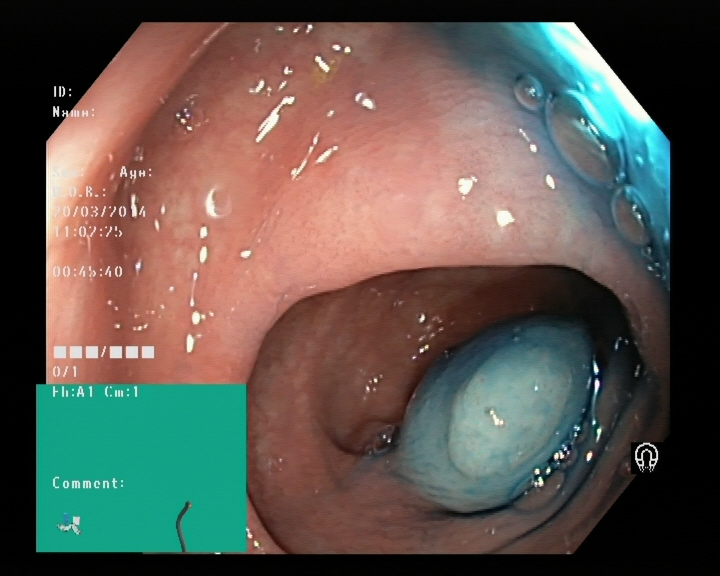
\includegraphics[width=\textwidth]{experiments/images/dyed-lifted-polyps.jpg}
            \caption{{\small Dyed lifted polyps }}    
            \label{fig:kvasir-dyed-lifted-polyps}
        \end{subfigure}
        \qquad
        \begin{subfigure}[b]{0.4\textwidth}  
            \centering 
            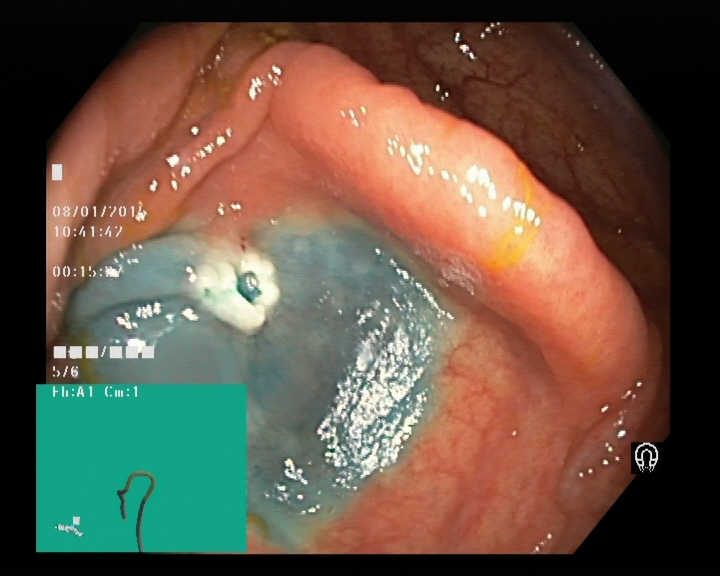
\includegraphics[width=\textwidth]{experiments/images/dyed-resection-margins.jpg}
            \caption{{\small Dyed resection margins }}    
            \label{fig:kvasir-dyed-resection-margins}
        \end{subfigure}
        \qquad\vfill%\vskip\baselineskip
        \begin{subfigure}[b]{0.4\textwidth}   
            \centering 
            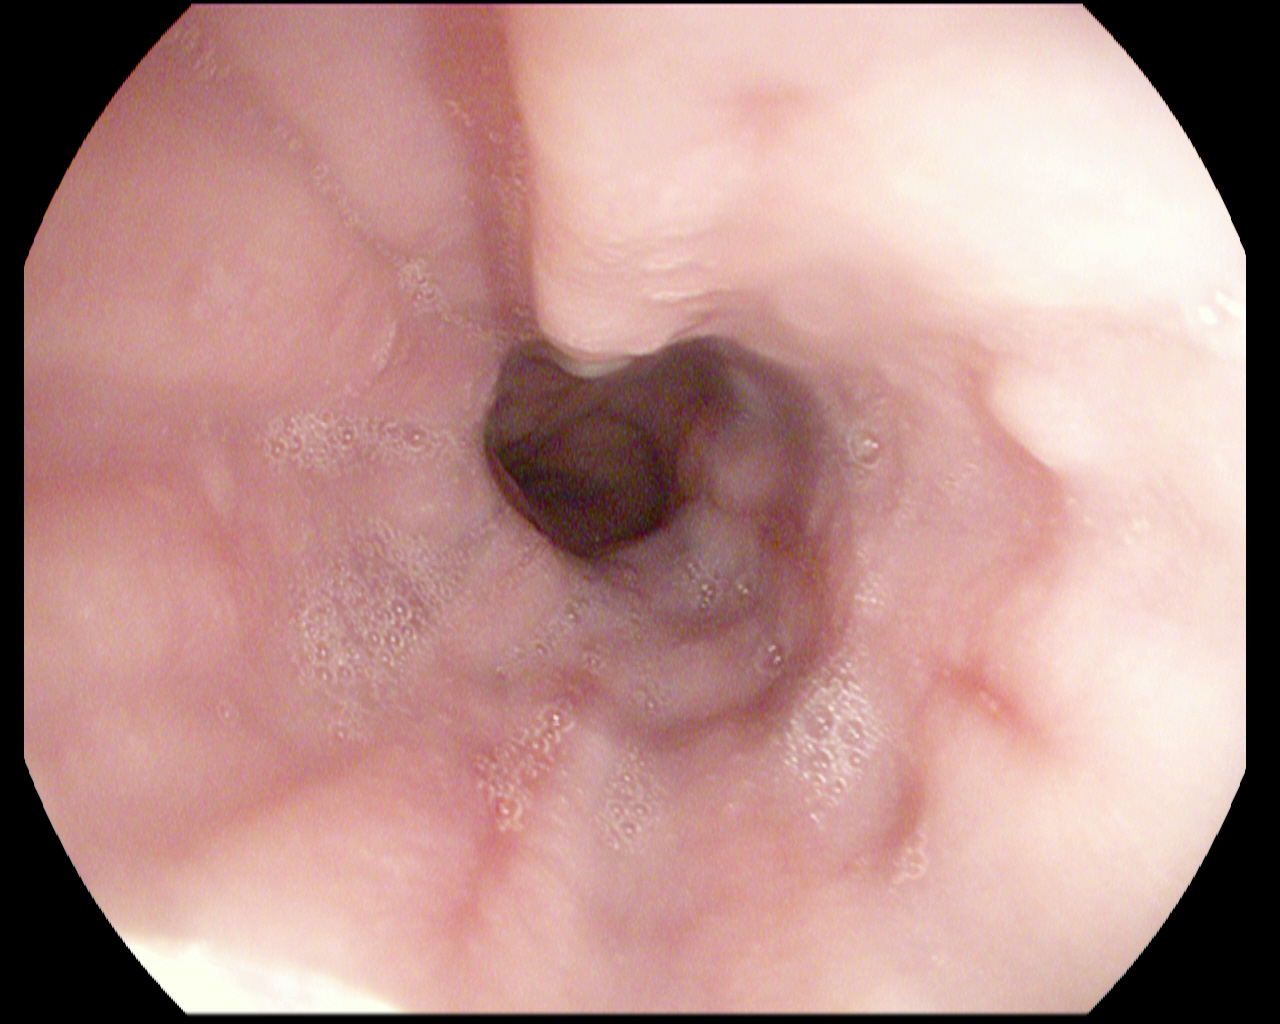
\includegraphics[width=\textwidth]{experiments/images/esophagitis.jpg}
            \caption{{\small Esophagitis}}    
            \label{fig:kvasir-esophagitis}
        \end{subfigure}
        \qquad%\hfill%\quad
        \begin{subfigure}[b]{0.4\textwidth}   
            \centering 
            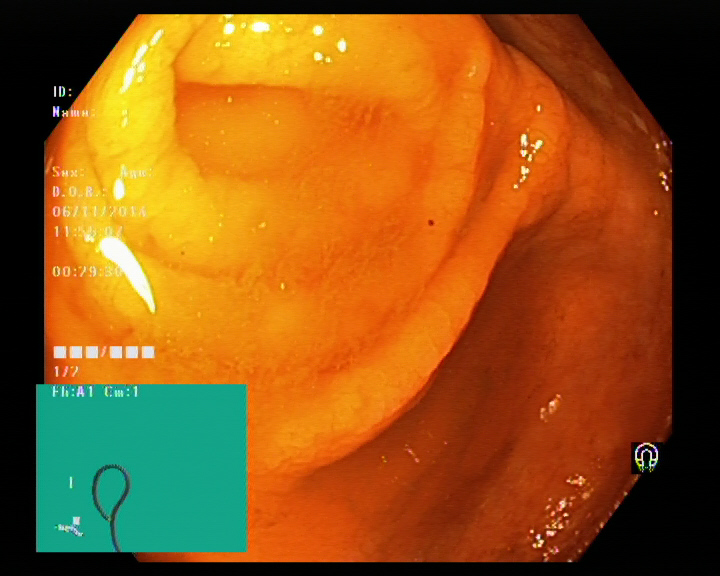
\includegraphics[width=\textwidth]{experiments/images/normal-cecum.jpg}
            \caption{{\small Normal cecum}}    
            \label{fig:kvasir-normal-cecum}
        \end{subfigure}
        \qquad
        \begin{subfigure}[b]{0.4\textwidth}
            \centering
            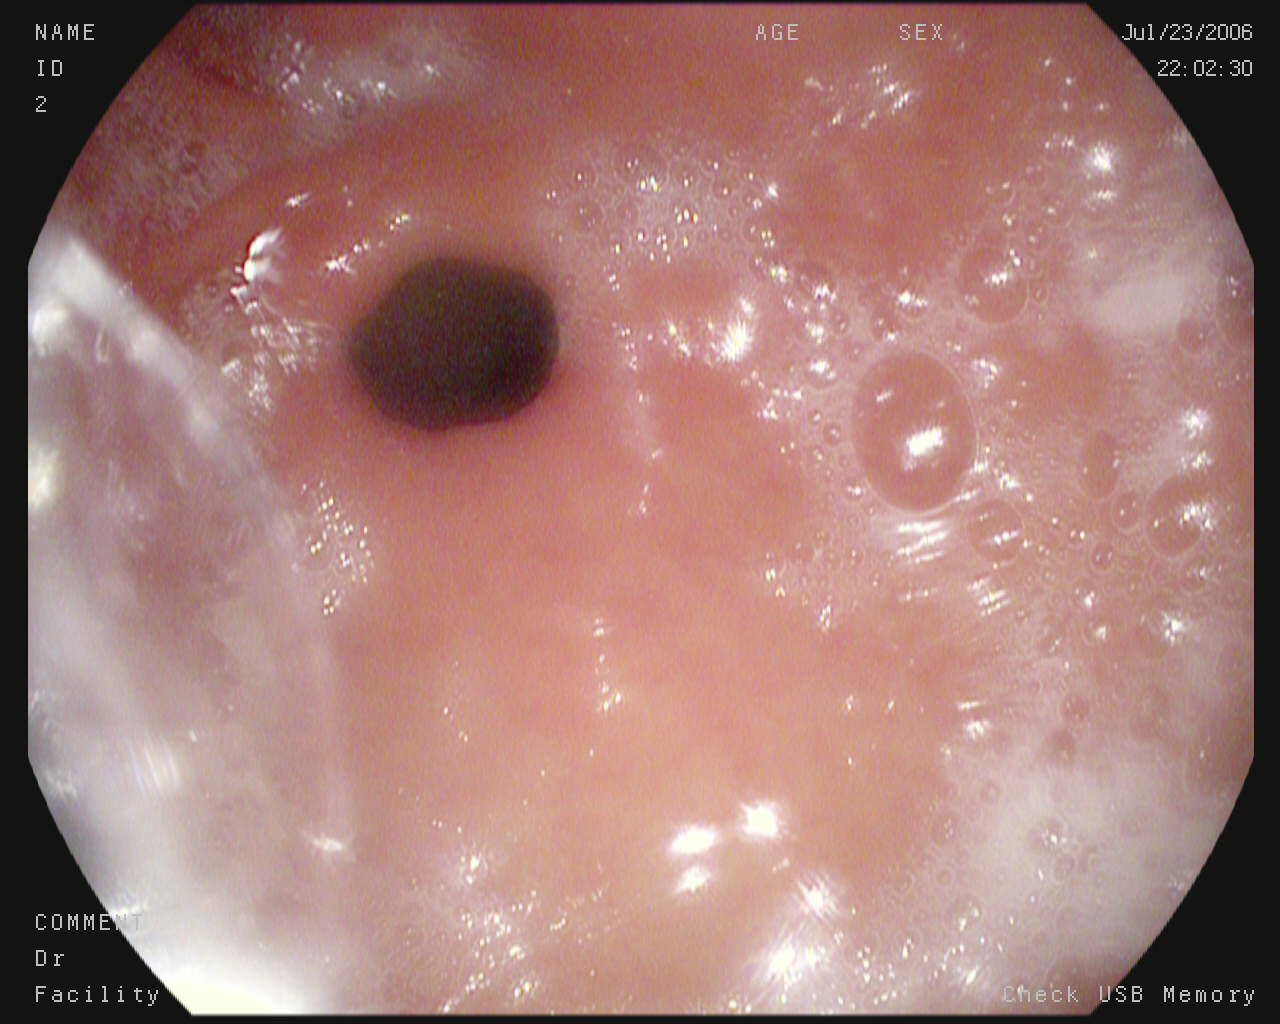
\includegraphics[width=\textwidth]{experiments/images/normal-pylorus.jpg}
            \caption{{\small Normal pylorus }}    
            \label{fig:kvasir-normal-pylorus}
        \end{subfigure}
        \qquad
        \begin{subfigure}[b]{0.4\textwidth}  
            \centering 
            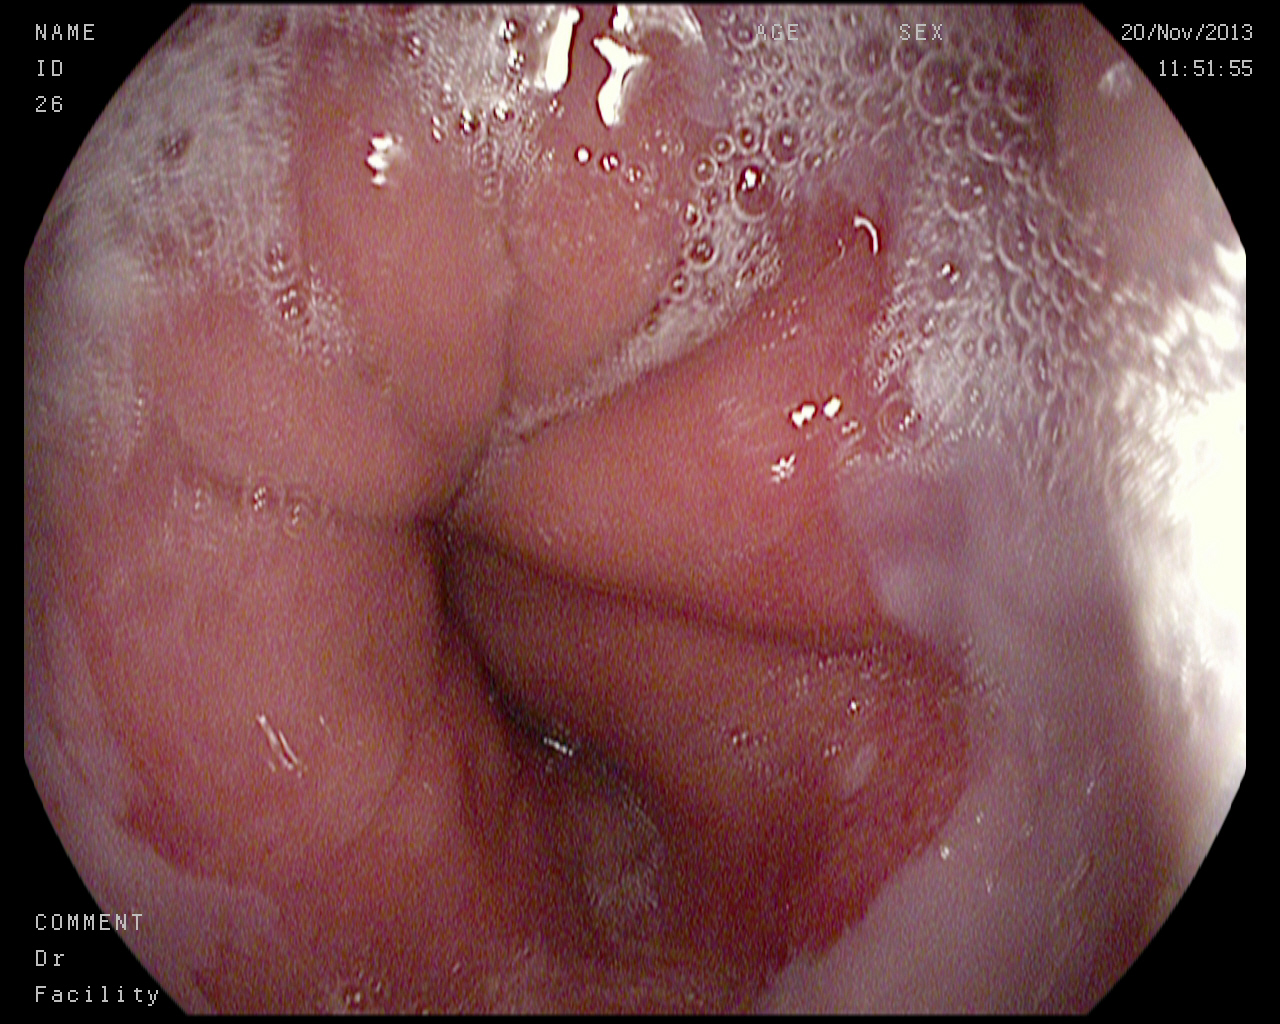
\includegraphics[width=\textwidth]{experiments/images/normal-z-line.jpg}
            \caption{{\small Normal z line}}    
            \label{fig:kvasir-normal-z-line}
        \end{subfigure}
        \qquad\vfill%\vskip\baselineskip
        \begin{subfigure}[b]{0.4\textwidth}   
            \centering 
            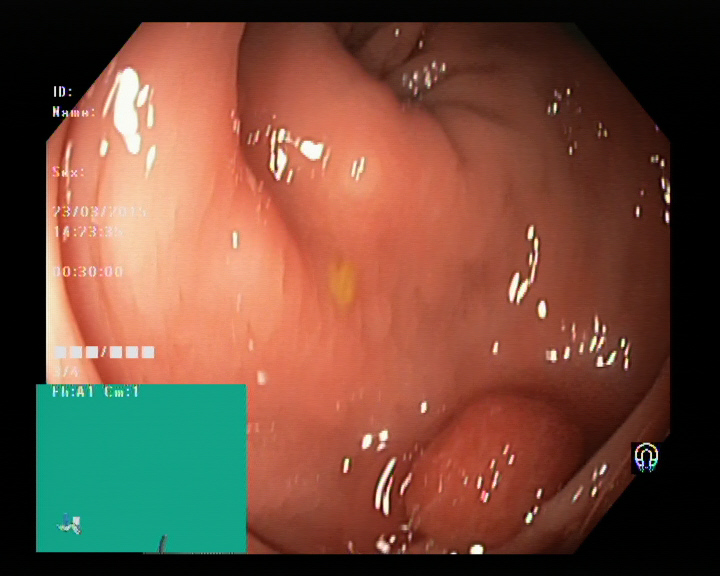
\includegraphics[width=\textwidth]{experiments/images/polyps.jpg}
            \caption{{\small Polyps}}    
            \label{fig:kvasir-polyps}
        \end{subfigure}
        \qquad%\hfill%\quad
        \begin{subfigure}[b]{0.4\textwidth}   
            \centering 
            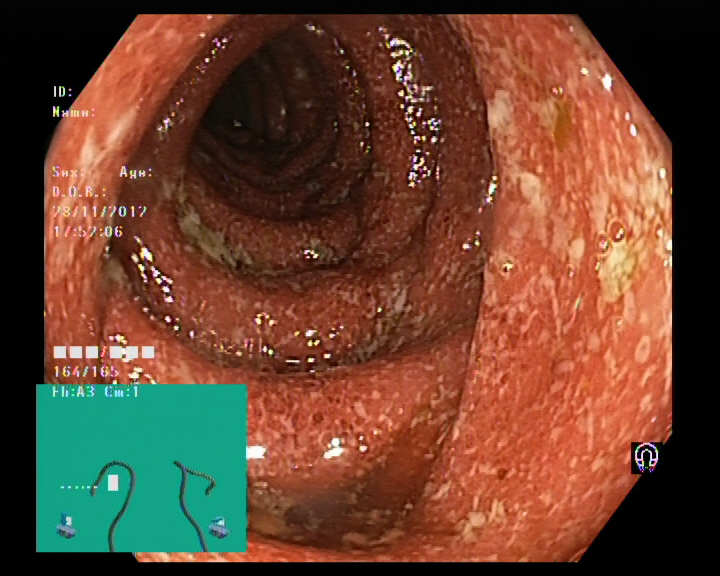
\includegraphics[width=\textwidth]{experiments/images/ulcerative-colitis.jpg}
            \caption{{\small ulcerative-colitis}}    
            \label{fig:kvasir-ulcerative-colitis}
        \end{subfigure}
        \caption{\small The Kvasir dataset with each of the eight classes} 
        \label{fig:Kvasir}
    \end{figure}
    



    \begin{figure}
        \centering
        \begin{subfigure}[b]{0.45\textwidth}
            \centering
            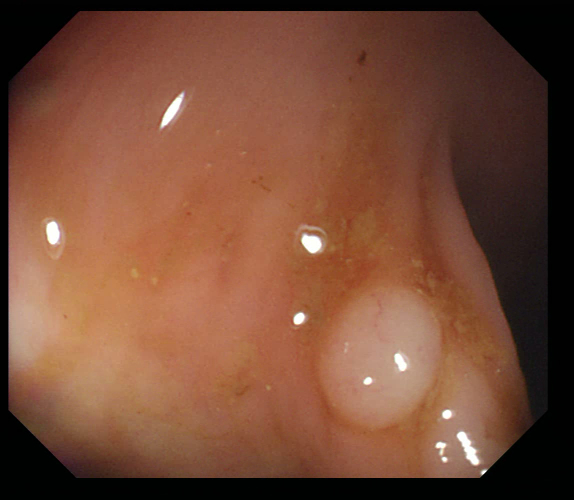
\includegraphics[height=5.5cm,width=\textwidth]{methodology/figures/CVC356polyp.jpg}
            \caption{{\small Polyp }}    
            \label{fig:CVC356polyp}
        \end{subfigure}
        \qquad
        \begin{subfigure}[b]{0.45\textwidth}  
            \centering 
            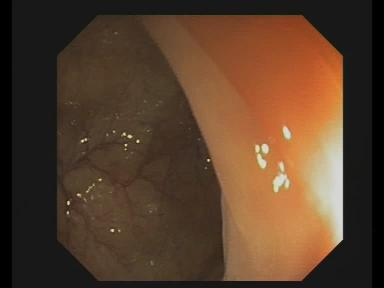
\includegraphics[height=5.5cm,width=\textwidth]{methodology/figures/CVC356NONpolyp.jpg}
            \caption{{\small Non-polyp }}    
            \label{fig:CVC356NONpolyp}
        \end{subfigure}
         \caption{\small The two classes from the CVC 356 dataset} 
        \label{fig:CVC356}
	\end{figure}
        
    \begin{figure}
        \centering       
        \begin{subfigure}[b]{0.45\textwidth}   
            \centering 
            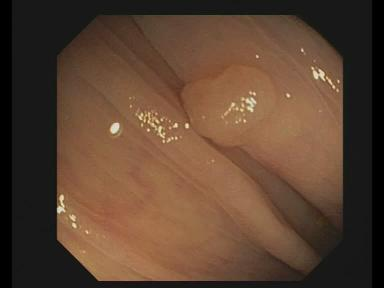
\includegraphics[height=5.5cm,width=\textwidth]{methodology/figures/CVC12kpolyp.jpg}
            \caption{{\small Polyp}}    
            \label{fig:CVC12kpolyp}
        \end{subfigure}
        \qquad%\hfill%\quad
        \begin{subfigure}[b]{0.45\textwidth}   
            \centering 
            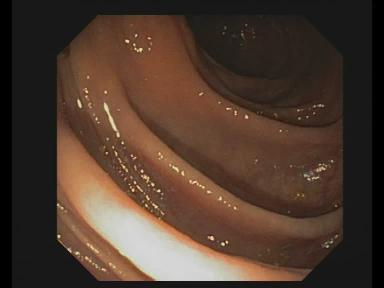
\includegraphics[height=5.5cm,width=\textwidth]{methodology/figures/CVC12kNONpolyp.jpg}
            \caption{{\small Non-polyp}}    
            \label{fig:CVC12kNONpolyp}
        \end{subfigure}
        \caption{\small The two classes from the CVC 12k dataset} 
        \label{fig:Kvasir}
    \end{figure}
    

    %=============================================
\FloatBarrier
\section{Metrics}
To discern the results of our experiments we introduce multiple metrics and tables to get an indication of our success. The primary dataset we used for training, Kvasir, was split into k number of folds, using k-fold cross-validation.  K-fold cross-validation is a tool used in statistics and machine learning to help to get an accurate representation of the data based on finding a statistical average of the dataset.  In machine learning, it is a powerful tool that can help with adapting to new datasets and prevent overfitting.  We recall that the Kvasir dataset contains 8000 images, with 1000 of each class.
In our testing, we split the dataset up in k=6 folds. This split means that we split our dataset into six pieces before training.  With the six folds, we assign one of them as a test set, and we assign the four other for training and validation. We then train our data five times, using four folds for training and the last fold for validation during training. For each training run, we rotate the validation set, so each of the five folds is used for validation once.


\begin{figure}[h]
\hspace*{-1cm}                                                           
\centering
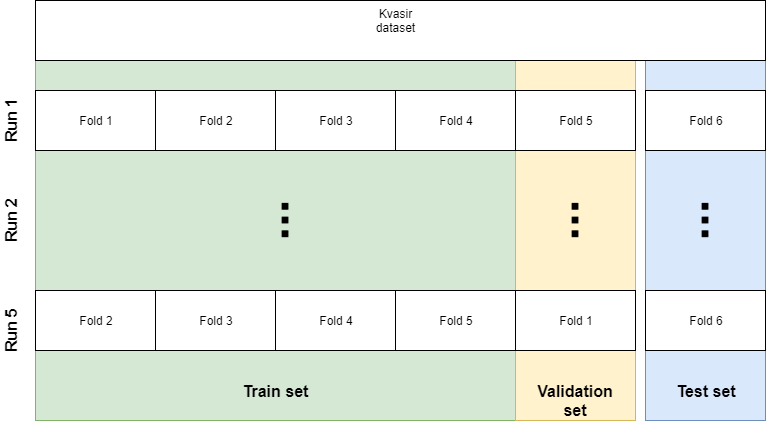
\includegraphics[scale=0.4]{experiments/figures/KfoldKvasir_compressed.png}
\caption{The Kvasir divided in to 6 folds}
\label{fig:KfoldKvasir}
\end{figure}

The advantage of using K-fold cross-validation is that we maximise the utility of the dataset. We find the distribution of the dataset that hopefully covers the most significant range of the unseen data. 

\subsection{The confusion matrix}
With k-fold cross-validation, we end up with the dataset that scored the highest during the final validation step.  There are multiple ways to calculate metrics for how well a dataset is doing,  but they all are a comparison of the predicted class versus the true class.  

Take for instance the case with the 8-class dataset Kvasir, where we predict an image to be normal-cecum. We translate this to an integer representation of, for instance, class 3. In our example, the actual True class is normal-z-line, here represented as 5. 

We can represent this as 
\[
\begin{bmatrix}
 3 & 5\\ 
\end{bmatrix}
\]
Storing value pairs like this can very quickly get cluttered and unorganised.
The most common way to store these value pairs is to use a confusion matrix.  We initiate the matrix as a \textit{$N \times N$} matrix where N is the total number of classes as shown in Figure \ref{mat:emptyCM}

\begin{figure}[h]
    \myfontsize
    \centering
    \[
    \begin{bmatrix}
     0 & 0 &  0 &  0 &  0 &  0 &  0 &  0\\
     0 & 0 &  0 &  0 &  0 &  0 &  0 &  0\\
     0 & 0 &  0 &  0 &  0 &  0 &  0 &  0\\
     0 & 0 &  0 &  0 &  0 &  0 &  0 &  0\\
     0 & 0 &  0 &  0 &  0 &  0 &  0 &  0\\
     0 & 0 &  0 &  0 &  0 &  0 &  0 &  0\\
     0 & 0 &  0 &  0 &  0 &  0 &  0 &  0\\
     0 & 0 &  0 &  0 &  0 &  0 &  0 &  0\\
    \end{bmatrix}
    \]
    \caption{An empty confusion matrix}
    \label{mat:emptyCM}
\end{figure}



After we have initialised the confusion matrix, we add each value pair as to the matrix at its corresponding position.  
Given the pair $\begin{bmatrix} 3 & 5 \end{bmatrix}$ we add one to the position corresponding to (x=3,y=5). 
Another example could be given the pair where we guessed class 0 and the true class was 0:  $\begin{bmatrix}  0 & 0 \end{bmatrix}$, we add one to the matrix at position (x=0,y=0). With the two examples we get the following confusion matrix as shown in Figure \ref{mat:nonemptyCM}

\begin{figure}[h]
    \myfontsize
    \centering
    \[
    \begin{bmatrix}
     1 & 0 &  0 &  0 &  0 &  0 &  0 &  0\\
     0 & 0 &  0 &  0 &  0 &  0 &  0 &  0\\
     0 & 0 &  0 &  0 &  0 &  0 &  0 &  0\\
     0 & 0 &  0 &  0 &  0 &  0 &  0 &  0\\
     0 & 0 &  0 &  0 &  0 &  0 &  0 &  0\\
     0 & 0 &  0 &  1 &  0 &  0 &  0 &  0\\
     0 & 0 &  0 &  0 &  0 &  0 &  0 &  0\\
     0 & 0 &  0 &  0 &  0 &  0 &  0 &  0\\
    \end{bmatrix}
    \]
    \caption{The confusion matrix with [3 5] and [0 0] inserted }
    \label{mat:nonemptyCM}
\end{figure}

As we fill in the matrix with more predictions, we can start to infer properties of the classifier. After approximately 1600 evaluations, our result might at the end look like Figure \ref{mat:FullCM}.
\begin{figure}[h]
    \myfontsize
    \centering
    \[
    \begin{bmatrix}
     195 & 50 &  0 &  0 &  0 &  0 &  2  & 1\\
       4 & 148&  1 &  0 &  0 &  0 &  0  & 0\\
       0 &  0 & 152&  0 &  3 & 40 &  0  & 5\\
       0 &  1 &  0 &198 &  0 &  0 & 13  & 4\\
       0 &  0 &  0 & 0  &195 &  1 &  5  & 2\\
       0 &  0 & 47 & 0  &  1 &159 &  0  & 0\\
       1 &  0 &  0 & 0  &  0 &  0 & 172 &  8\\
       0 &  1 &  0 & 2  &  1 &  0 &  8  & 180\\
    \end{bmatrix}
    \]
    \caption{The confusion matrix with  almost 1600 predictions}
    \label{mat:FullCM}
\end{figure}
We can see that the majority of predictions lie around the diagonal. This centralisation means that most of our results were classified correctly, as values at the diagonal are the same x and y values, and subsequently a correct prediction. 
We can also discern something about the four primary metrics associated with a value in the matrix.\\

\textbf{True Positive (TP): } True positive for a class is when the sample is predicted positive, and the True label is also positive.  In the Kvasir dataset, we have a True positive result if, for the class polyp, we predict a polyp.\\

\textbf{True Negative (TN): } True Negative is the opposite of true positive. Given the class Polyp from the Kvasir dataset, we guess that the image is not a polyp when the True label is non-polyp. 

\textbf{False Positive (FP): } False positive is, given a True label, we predict it to be False. We often call this type of error a "Type 1 error".   In the polyp case, this is the case where we predict a polyp when there is no polyp present.

\textbf{False Negative (FN): } False positive is the case where we fail to predict the class when it is True. We call this error for "Type 2 error". False Negative is, in our case, the least desirable outcome for our classes with pathological findings like Esophagitis, Polyps and Ulcerative Colitis.

\vspace{5px}
The metrics described is in the case of ``single class'' labelling. In most medical cases we often want to use more than two classes for the data. 
When labelling data based on multiple classes we use the metrics as shown in Figure \ref{fig:confusionmatrix_labels}, here we can see that for a given class we only have one option for True positive, and the diagonal and horizontal represent False positive and False Negative respectively. The rest of the options are True negative. 
\begin{figure}[h]
\centering
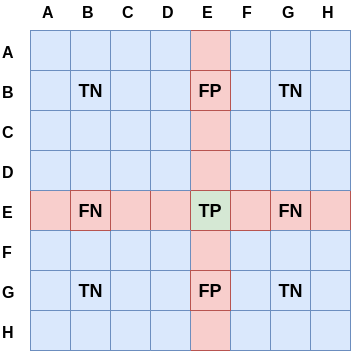
\includegraphics[scale=0.7]{experiments/figures/confusionmatrix.png}
\caption{
Confusion matrix with eight classes, here True positive is marked in green, False Negative and False positive marked in red, and True negative in blue.
}
\label{fig:confusionmatrix_labels}
\end{figure}


\subsection{Common metrics}
\label{cha:metrics}
When evaluating our results, we use a set of common metrics used in the field of statistics and machine learning.  The metrics we will be using in this thesis are Recall (REC), Precision (PREC), Specificity (SPEC), Accuracy (ACC), Matthews correlation coefficient (MCC), and F1 score (F1). 


\vspace{5px}
\paragraph{Accuracy:}  
Accuracy is the percentage of the predictions that were classified correctly.
It describes how many of our predictions were correct out of the total predictions made as shown in equation \ref{eq:ACC}. It is the most common metric given its simplicity both in calculation and understanding. 
In general when our data is balanced, and we only have a few classes, we can get away with using accuracy.
A pitfall with the accuracy metric is the lack of a comprehensive overview of the data, as it is just a summation without respect to classes involved.
In this project, we use accuracy during the training step as a metric of success. After training is complete, we do not use accuracy as an indication of success given our unbalanced datasets. 
 \begin{equation}
ACC=\frac{TP+TN}{TP+TN+FP+FN}
\label{eq:ACC}
\end{equation}

\vspace{5px}
\textbf{Recall:}  
Recall is the probability of detection, often called sensitivity.
This metric is a measure of the fraction of relevant instances that have been retrieved over the total amount of relevant instances for a binary classification example. It is calculated using equation \ref{eq:REC}.

Recall together with Specificity and Precision gives a complete view of the data compared to for instance accuracy alone. This difference is shown when we have uneven datasets. Given a dataset where we know that only 1\% of the data is negative, we will get an accuracy of 99\% if we label all the data as positive. When adding recall, specificity and precision, our score will reflect that we mislabeled all the negative values.
%\todo{ "Detector Performance Analysis Using ROC Curves – MATLAB & Simulink Example". www.mathworks.com. Retrieved 11 August 2016.}
\begin{equation}
REC=\frac{TP}{TP+FN}
\label{eq:REC}
\end{equation}




\vspace{5px}
\textbf{Specificity:} Specificity measures the proportions of our samples that were correctly identified as negative, when the true class were also negative. 
Specificity is related to recall as an opposite in the binary class example.
Equation \ref{eq:SPEC} shows the equation used for specificity.
\begin{equation}
TPR=\frac{TN}{TN+FP}
\label{eq:SPEC}
\end{equation}



\vspace{5px}
\textbf{Precision:}
Precicion is the meassure of relevance in the binary classification case.
As we can see from equation \ref{eq:PREC} the formula is similar to recall, but it only looks at the positive samples. 
\begin{equation}
PREC=\frac{TP}{TP+FP}
\label{eq:PREC}
\end{equation}



\vspace{5px}
\textbf{F1 score:}
F1 score is a combination of precision and recall as shown in equation \ref{eq:F1}.

\begin{equation}
F1=\frac{precision \times recall}{precision + recall}
\label{eq:F1}
\end{equation}



\vspace{5px}
\textbf{Matthews correlation coefficient:}
Matthews correlation coefficient is a metric that takes all four possible states of TP, TN, FN and FP in to account. As with the F1 score, the Matthews correlation coefficient gives a score that is based on a more complete understanding of the data compared to how metrics like recall and precision only looks at a subset of the data.

Equation \ref{eq:MCC} shows the formula. It can output a score from -1 to 1, where 1 is a correct classification and -1 a total incorrect prediction. A score of 0 shows no statistical relevance in the result we have.
\begin{equation}
MCC=\frac{TP \times TN - FP \times FN}{\sqrt{(TP + FP)(TP + FN)(TN + FP)(TN + FN)}}
\label{eq:MCC}
\end{equation}







\subsection{Singleclass vs Multiclass Metrics}

The metrics presented are, in general, a solid way to present the validity of a model. However, not all metrics presented is the same when switching between single and multiclass classification.  Metrics like Accuracy is designed to work for multiclass classification, given that there is only one way to calculate the score as shown in either equation \ref{eq:ACC} or in equation \ref{eq:ACCalt}.
\begin{equation}
\frac{\sum (diag(Covarience Matrix))}{\sum(Covariance Matrix)}
\label{eq:ACCalt}
\end{equation}

The problem with multiclass metrics arises when there is more than one way to calculate the metrics needed, this can be for instance Recall and Specificity, where we have multiple ways to add together the class-wise scores. The three most common ways to calculate the average are:

\textbf{Micro average}: calculates the mean value of each of the binary metrics and averages the result over the total number of samples. 
Micro average ignores all class frequencies and gives us a metric based on all samples gathered. Micro-averaging may be preferred in multilabel settings, including multiclass classification where a majority class is to be ignored.\\

\textbf{Macro average}: calculates the mean of each of the binary metrics, giving the same weight to each of the classes. Macro average gives importance to classes with few samples, and infrequent classes play the same roles as frequent ones. The disadvantage with Macro average is the fact that in the real world some classes often plays a more significant role than others, and doing especially bad on one of the classes can worsen the total result. \\

\textbf{Weighted average} calculates the mean of each of the binary metrics but gives a weighted sum for each of the scores before it is averaged. 
The weight of each class depends on the size of the true data samples.
The weighted average gives us the advantage that small classes still count more than it would with for instance Micro average, but since it depends on the number of samples from each class it can end up more or less as a black box during calculation.
Weighted average gives us the best of both worlds, but it lacks the intuitiveness from the two other classes. \\

With the three methods presented, we have chosen to Macro average our results. While both Macro and Weighted average would give a good indication given that not all our datasets are balanced, we argue that the weighted average would give metrics that are harder to explain when we are working on datasets with unbalanced classes.

In addition to looking at the Macro average of precision and recall, we want to look at specific cases of the classification.  In many cases, we have multiple classes, where we are most interested in just one or a handful of the classes shown. 
For instance, a focus we have in this thesis is to give a score on how predictable polyp detection is, and on that case, we want to discuss the True positive rate (TPR) of the polyp detection and not the TPR of the non-polyp classes. 

\todo{Might remove rest of this section.. Need to think about it.}
Take for instance the matrix \ref{mat:exampleMAT}\\
\begin{figure}[h]
    \centering
	\[
	\begin{bmatrix}
	 10 & 1 \\
	 3 & 12 \\
	\end{bmatrix}
	\]
    \caption{Nearly balanced matrix}
    \label{mat:exampleMAT}
\end{figure}



Here we can calculate the weighted average recall to be \todo{x}. This can be an interesting observation in itself, but often the first or second True label is much more important relative to the other.  In a more practical example: We are more interested in finding areas with polyps when we know they are present, compared knowing there is not a polyp in an area when none are present. 

These Metrics becomes a more prominent topic when it comes to inpainting. With inpainting, we take areas with no relevant information and makes it into areas that are similar to the rest of the image. Given that we can inpaint over polyps by mistake, or that we might train our classifiers to not look in certain areas when classifying, we have an interest if also comparing single cases of recall and precision included to the average values.


\subsection{Hardware and Software setup}
For the experiments we used the hardware setup shown in table \ref{tab:HW}.
The software type and version for the experiments is shown in table \ref{tab:SW}.


\begin{table}[]
\centering
\begin{tabular}{@{}cc@{}}
\toprule
\multicolumn{1}{c}{Name} & \multicolumn{1}{c}{Version} \\ \midrule
Ubuntu                   & 18.04.2                 \\
Python                   & 3.6.7                       \\
Tensorflow               & 1.13.0                      \\
Keras                    & 2.2.4                       \\
CUDA                     & 10.0.130                    \\
cuDNN                    & 7                           \\ \bottomrule
\end{tabular}
\caption{Software specifications for our system}
\label{tab:SW}
\end{table}

\begin{table}[]
\centering
\begin{tabular}{@{}cc@{}}
\toprule
\multicolumn{1}{c}{Category} & \multicolumn{1}{c}{Name}       \\ \midrule
CPU                          & Intel i5-4590 CPU @ 3.30GHz    \\
GPU                          & Nvidia GeForce GTX 1080 TI     \\
RAM                          & Kingston 16 GB DDR3 @ 1600 MHz \\ \bottomrule
\end{tabular}
\caption{Hardware specifications for our system}
\label{tab:HW}
\end{table}

\todo{MICHAEL OR PAAL: \\ Do I need more info/fluff here? }

\section{Setup of experiments}
As we recall, we proposed the following hypothesis.
\vspace{10px}

\noindent
\textbf{Hypothesis \ref{hyp:a}:}
When classifying images, we will get the best result when we have images with the least amount of sparse information.
Hence, by removing areas with sparse information, we will see an increase in classification performance compared to not removing the areas.

\vspace{5px}


\noindent 
\textbf{Hypothesis \ref{hyp:b}:}
When training a classifier, we will get a higher probability of generalisation of our results when removing the dataset-specific artefacts compared to not removing artefacts.
\vspace{5px}

In this thesis we use the hypothesises as the basis to solve the problem statements. 
We divide our work into two parts, inpainting and classifying. 
First, we will look at the process of inpainting in detail, and inspect the results we have.  
We will look at how parameters affect the results, and how different networks will differ in the generating process. \todo{more}


After a rundown of the generation of the custom datasets trough inpainting, we will show how the classification scores for each of the created dataset. Here we look at the datasets generated by inpainting and compare them with a base case. 

Our primary goal in this thesis is to see if any of the generated datasets can help with classification. We will both compare the different areas inpainted, and the method used to inpaint the images. 
For the classification, we will use MCC as our primary metric for comparison, as described in section \ref{cha:metrics}. As we described in the MCC paragraph, this metric gives us the best indication of success based on the imbalance of data in the CVC datasets. We chose to show the other metrics from section \ref{cha:metrics} as well, but they are only there to get a comprehensive picture of the results.




\section{Results of the Inpainting}
We will first take a look at the generation of the new datasets and the machine learning methods used to inpaint the problematic areas.

We can recall that based on  Hypothesis \ref{hyp:a}, we can assume that the removal of areas with sparse information we achieve a higher classification score. We have chosen our first dataset to contain the images from the Kvasir dataset where the black corners and edges inpainted. 
From this, we hypotosise that we will see an increase in classification when training and testing on the same dataset, as well when testing on a new dataset, given that the network has less sparseness to take into account. 

Based on Hypothesis \ref{hyp:b}, we predict assume that the removal of areas with dataset specific artefacts will result in a higher classification score.  By removing the green squares in the corners and the text overlayed on top of the images, we predict that we get a higher classification score on previously unseen datasets compared to not removing dataset specific artefacts.


With Hypothesis \ref{hyp:a} and \ref{hyp:b} in mind, we present three types of datasets with two different generators to see if our hypothesises are correct. The full list of datasets is shown in Figure \ref{tab:datasets}




\begin{table}[h]
\centering
\footnotesize
\caption*{\small \textbf{BC}: Black corner. \textbf{GS}: Green square. \textbf{BC+GS}: Black corner and Green square}
\begin{tabular}{lccc}
\toprule
{Dataset labels} & {Size} & {Inpainted area} & {Generator network used} \\ 
\midrule
I    - Base Case                       & 256x256 px         & -        & -                   \\
II   - Autoencoder with black corner   & 256x256 px         & BC       & Autoencoder         \\
III  - Autoencoder with green square   & 256x256 px         & GS       & Autoencoder         \\
IV   - Autoencoder with both           & 256x256 px         & BC+GS    & Autoencoder         \\
V    - GAN with black corner           & 256x256 px         & BC       & GAN                 \\
VI   - GAN with green square   		   & 256x256 px         & GS       & GAN                 \\
VII  - GAN with both                   & 256x256 px         & BC+GS    & GAN                 \\
VIII - Base Case					   & 512x512 px         & -        & -                   \\
IX - Autoencoder with black corner     & 512x512 px         & BC       & Autoencoder         \\
X - Autoencoder with green square      & 512x512 px         & GS       & Autoencoder         \\
XI - Autoencoder with both   		   & 512x512 px         & BC+GS    & Autoencoder         \\
XII - GAN with black corner            & 512x512 px         & BC       & GAN                 \\
XIII - GAN with green square           & 512x512 px         & GS       & GAN                 \\
XIV - GAN with both           	  	   & 512x512 px         & BC+GS    & GAN                 \\
\bottomrule
\end{tabular}%
\caption{Details of all datasets we generate in the experiments.} 
\label{tab:datasets}
%\caption{\small BC: Black corner. GS: Green square. BC+GS: Black corner and Green square}
\end{table}

\FloatBarrier
\subsection{Black corners}
When generating the two first datasets (II \& V in Table \ref{tab:datasets}), we used the mask shown in Figure \ref{fig:CornerMask}. Here we did two operations, first cropping, then inpainting. The result is shown in Figure \ref{fig:AE_GAN_CORNER1} and Figure \ref{fig:AE_GAN_CORNER2}.

\begin{figure}
        \tiny
        \begin{subfigure}[t]{\myfigsizethree}
            \centering
            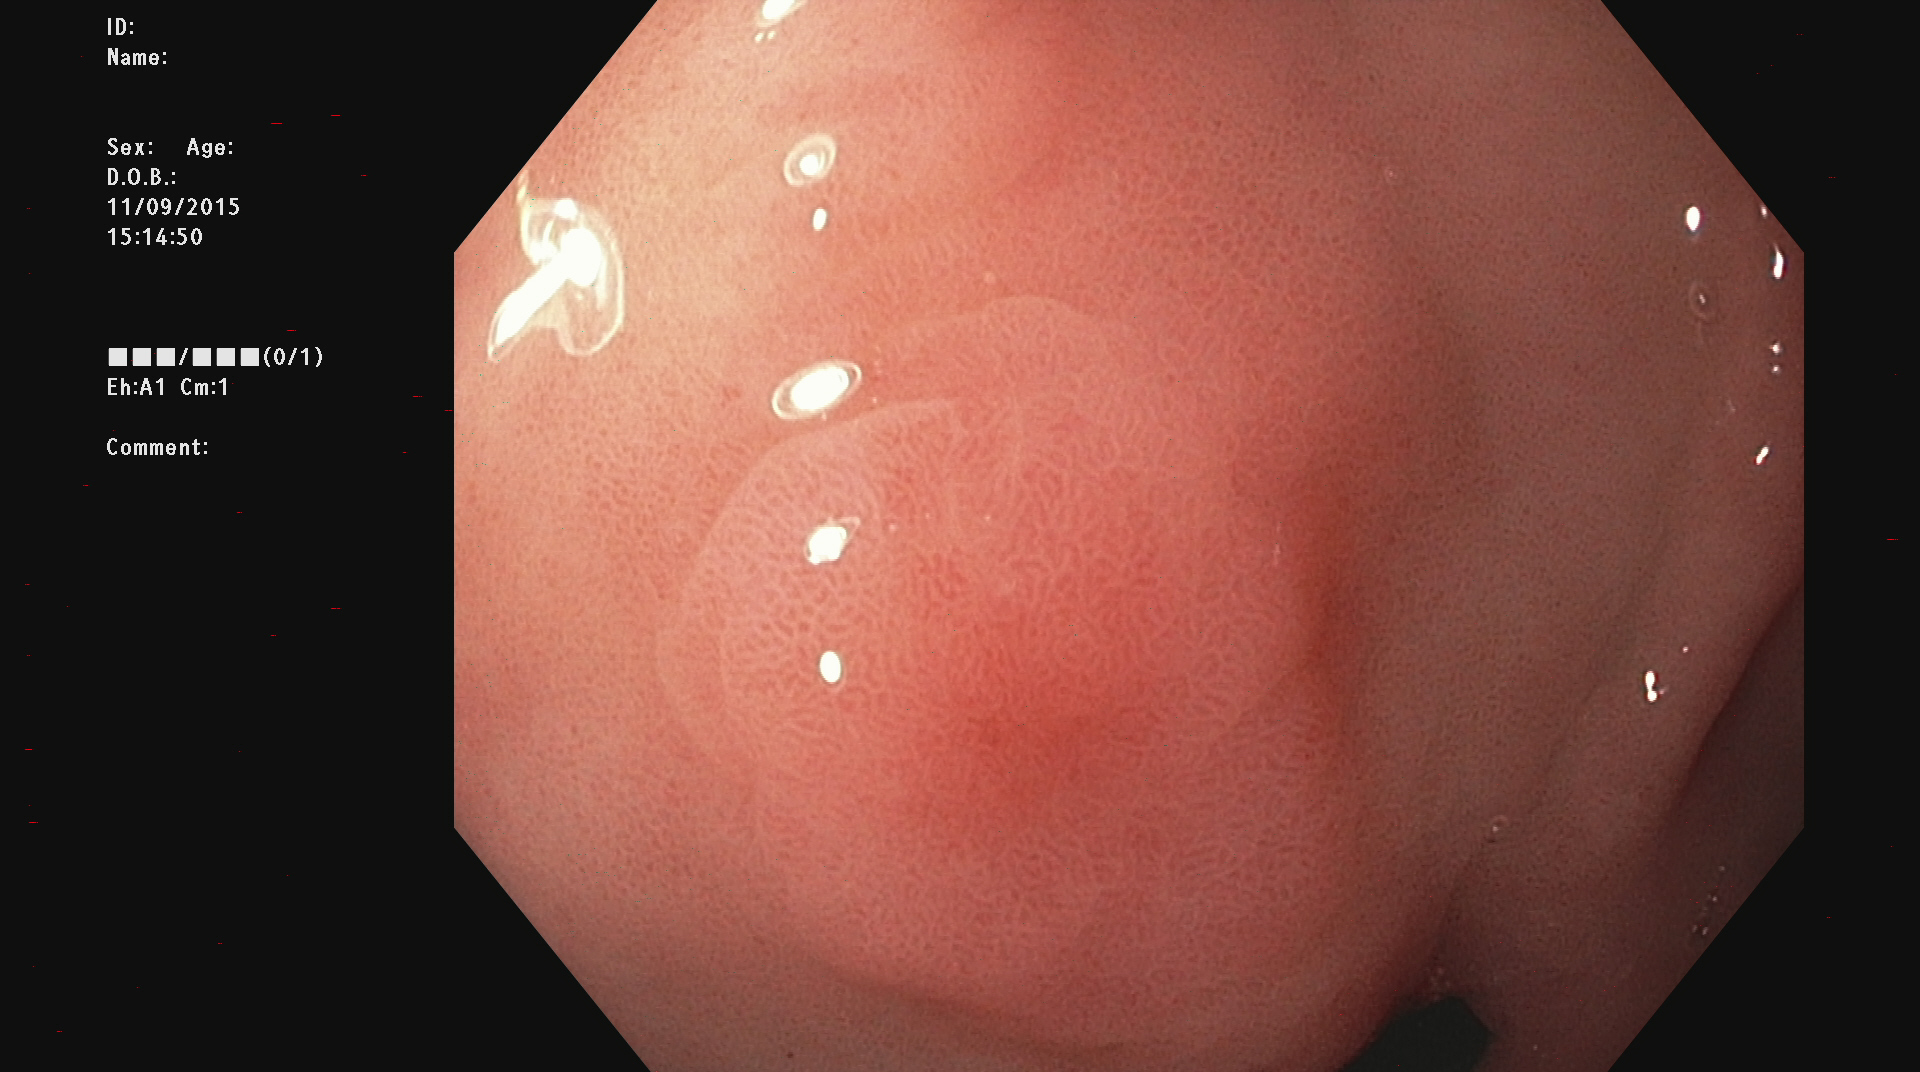
\includegraphics[height=\textwidth, width=\textwidth]{experiments/figures/blackcorner/polypORIG.jpg}
            \caption{Original polyp image }    
            \label{fig:polyp_ORIG_CORNER1}
        \end{subfigure}
        \qquad
        \begin{subfigure}[t]{\myfigsizethree}
            \centering
            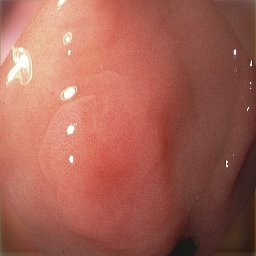
\includegraphics[width=\textwidth]{experiments/figures/blackcorner/polypAE.jpg}
            \caption{AE generated polyp image}    
            \label{fig:polyp_AE_CORNER1}
        \end{subfigure}
        \qquad
        \begin{subfigure}[t]{\myfigsizethree}  
            \centering 
            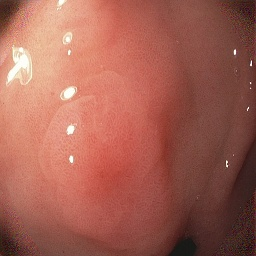
\includegraphics[width=\textwidth]{experiments/figures/blackcorner/polypGAN.jpg}
            \caption{GAN generated polyp image}    
            \label{fig:polyp_GAN_CORNER1}
        \end{subfigure}
        \qquad\vfill
       	\begin{subfigure}[t]{\myfigsizethree}   
            \centering 
            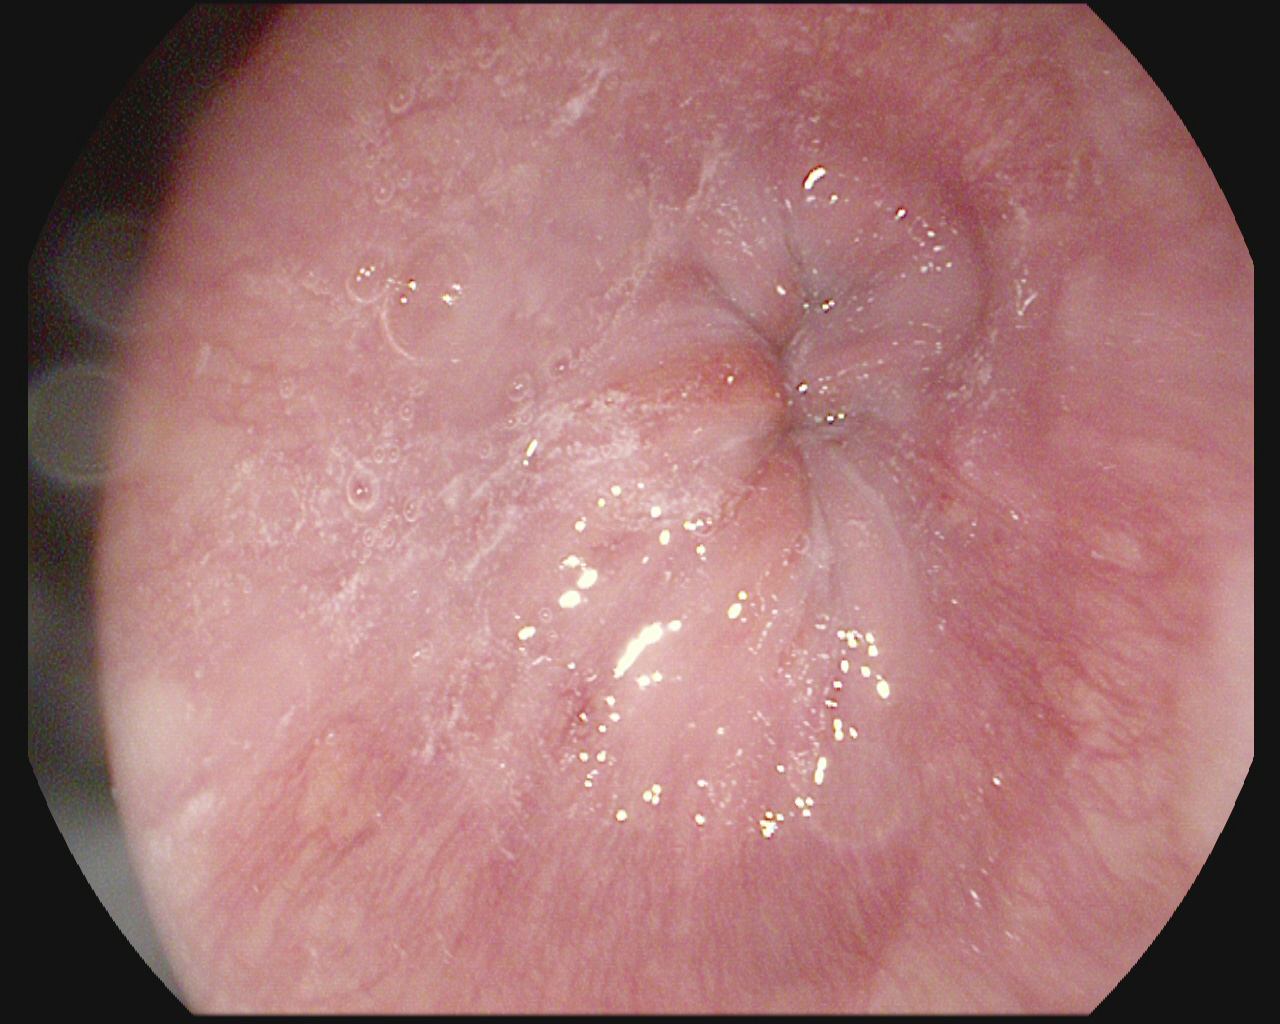
\includegraphics[height=\textwidth,width=\textwidth]{experiments/figures/blackcorner/zORIG.jpg}
            \caption{Original normal-z-line image }   
            \label{fig:z_ORIG_CORNER1}
        \end{subfigure}
        \qquad
        \begin{subfigure}[t]{\myfigsizethree}   
            \centering 
            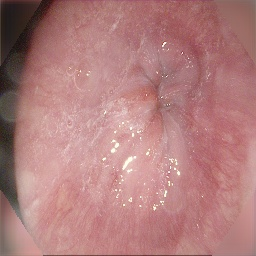
\includegraphics[width=\textwidth]{experiments/figures/blackcorner/zAE.jpg}
            \caption{AE generated normal-z-line image }   
            \label{fig:z_AE_CORNER1}
        \end{subfigure}
        \qquad%\hfill%\quad
        \begin{subfigure}[t]{\myfigsizethree}   
            \centering 
            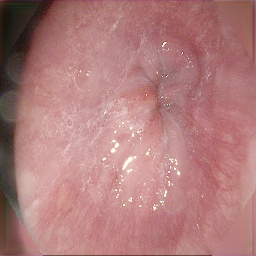
\includegraphics[width=\textwidth]{experiments/figures/blackcorner/zGAN.jpg}
            \caption{GAN generated normal-z-line class image}    
            \label{fig:z_GAN_CORNER1}
        \end{subfigure}
        \caption{Images from the polyp class and the z-line class. Both the AE and the GAN performed well in this scenario.} 
        %The images to the left is the original non-augmented images, the images in the middle were inpained with an Autoencoder, and the images on the right were inpainted with a GAN} 
        \label{fig:AE_GAN_CORNER1}
\end{figure}
    
\begin{figure}
        %\centering
        \tiny
        \begin{subfigure}[t]{\myfigsizethree}
            \centering
            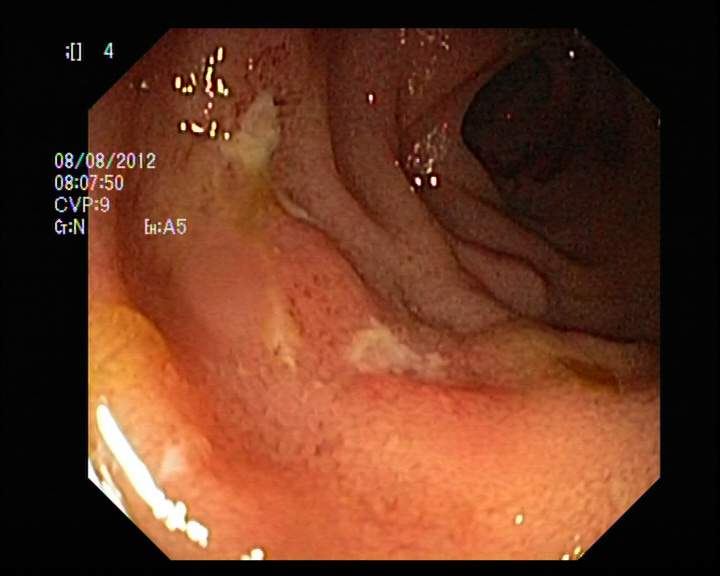
\includegraphics[height=\textwidth ,width=\textwidth]{experiments/figures/blackcorner/ucORIG.jpg}
            \caption{ Original ulcerative colitis image}    
            \label{fig:polyp_ORIG_CORNER2}
        \end{subfigure}
        \qquad
        \begin{subfigure}[t]{\myfigsizethree}
            \centering
            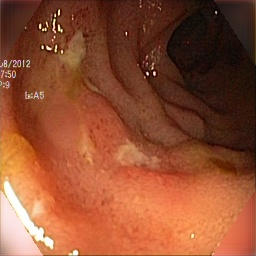
\includegraphics[width=\textwidth]{experiments/figures/blackcorner/ucAE.jpg}
            \caption{ AE generated ulcerative colitis image }    
            \label{fig:polyp_AE_CORNER2}
        \end{subfigure}
        \qquad
        \begin{subfigure}[t]{\myfigsizethree}  
            \centering 
            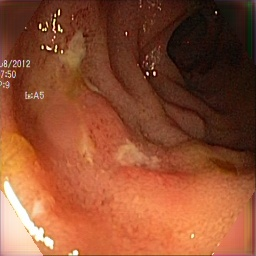
\includegraphics[width=\textwidth]{experiments/figures/blackcorner/ucGAN.jpg}
            \caption{ GAN generated ulcerative colitis image}   
            \label{fig:polyp_GAN_CORNER2}
        \end{subfigure}
        \qquad\vfill%\vskip\baselineskip
        \begin{subfigure}[t]{\myfigsizethree}   
            \centering 
            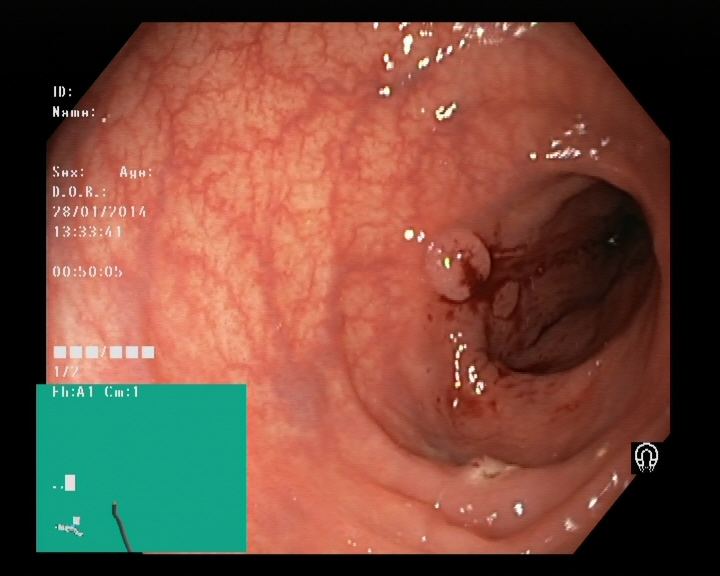
\includegraphics[height=\textwidth, width=\textwidth]{experiments/figures/blackcorner/polypwithgreenORIG.jpg}
            \caption{ Original polyp image }   
            \label{fig:z_ORIG_CORNER2}
        \end{subfigure}
        \qquad
        \begin{subfigure}[t]{\myfigsizethree}   
            \centering 
            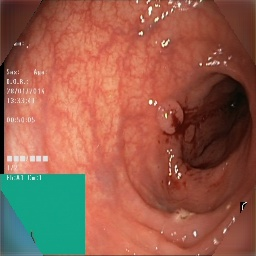
\includegraphics[width=\textwidth]{experiments/figures/blackcorner/polypwithgreenAE.jpg}
            \caption{AE generated polyp image }   
            \label{fig:z_AE_CORNER2}
        \end{subfigure}
        \qquad%\hfill%\quad
        \begin{subfigure}[t]{\myfigsizethree}   
            \centering 
            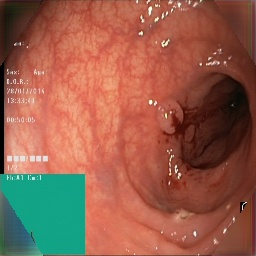
\includegraphics[width=\textwidth]{experiments/figures/blackcorner/polypwithgreenGAN.jpg}
            \caption{GAN generated polyp image}   
            \label{fig:z_GAN_CORNER2}
        \end{subfigure}
        \caption{Images from the polyp class and the ulcerative colitis. Here we see results that are not up to a good standard with regards to light and colours.} 
        \label{fig:AE_GAN_CORNER2}
\end{figure}
    
In Figure \ref{fig:AE_GAN_CORNER1} present representative images from both datasets inpainting the four edges around the image. Figure \ref{fig:AE_GAN_CORNER1} show images that, for both datasets, images are well inpainted, and a good portion could pass as real images. We can discern that, in general, the autoencoder dataset gives a much more blurry image compared to the dataset generated by the GAN. 

Figure \ref{fig:AE_GAN_CORNER2} show images that are more problematic. In Figure \ref{fig:polyp_AE_CORNER2} the image generated by the Autoencoder has drawn its colour from the nearby white over-saturated area, and subsequently, it has misdrawn the corner. In Figure \ref{fig:polyp_GAN_CORNER2} we do not have the same problem, as it has drawn information from a larger part of the image, and hence not drawn the oversaturated area.
Both models failed in getting the right colour for the green box when present. 
In general, we remove a lot of the areas with sparse information solely by cutting the black border of the image. The finished product is without any areas with sparse information, compared to for instance \ref{fig:polyp_ORIG_CORNER1}, where 25\% of the image contains no relevant information. 

\vspace{5px}
\noindent The training time for the AE regarding removing the black edges took under 4 hours. This wait, in the realm of machine learning, is fairly quick and based only on the training time, might be worth doing.
The training time of the GAN was over two days. The result of the GAN is a significant improvement over the AE, but might not be worth it at 12 times the training time. 


\FloatBarrier
\subsection{Green square}
The next two datasets (III \& VI in Table \ref{tab:datasets}) were generated from the mask in Figure \ref{fig:GreenMask}.  The goal of the datasets generated by the Autoencoder and the GAN is to remove the dataset-specific green square. The same cropping-inpainting procedure were applied. The result is shown in Figure \ref{fig:AE_GAN_SQUARE1} and Figure \ref{fig:AE_GAN_SQUARE2}.


\begin{figure}
        %\centering
                \tiny
        \begin{subfigure}[t]{\myfigsizethree}
            \centering
            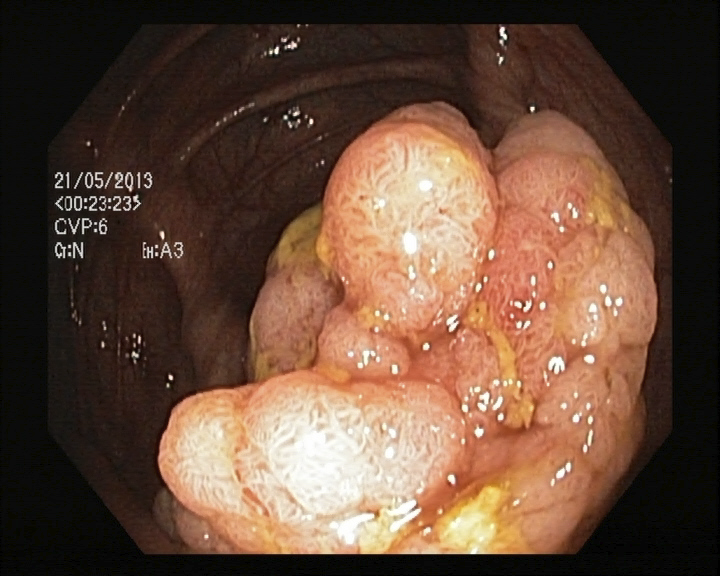
\includegraphics[height=\textwidth ,width=\textwidth]{experiments/figures/greensquare/polypORIG.png}
            \caption{Original polyp image }   
            \label{fig:polyp_ORIG_SQUARE1}
        \end{subfigure}
        \qquad
        \begin{subfigure}[t]{\myfigsizethree}
            \centering
            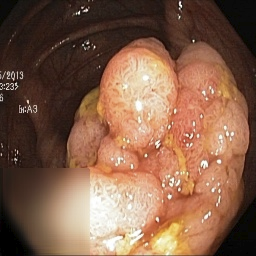
\includegraphics[width=\textwidth]{experiments/figures/greensquare/polypAE.png}
            \caption{AE generated polyp image }   
            \label{fig:polyp_AE_SQUARE1}
        \end{subfigure}
        \qquad
        \begin{subfigure}[t]{\myfigsizethree}  
            \centering 
            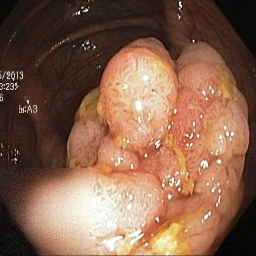
\includegraphics[width=\textwidth]{experiments/figures/greensquare/polypGAN.png}
            \caption{GAN generated polyp image}   
            \label{fig:polyp_GAN_SQUARE1}
        \end{subfigure}
        \qquad\vfill%\vskip\baselineskip
        \begin{subfigure}[t]{\myfigsizethree}   
            \centering 
            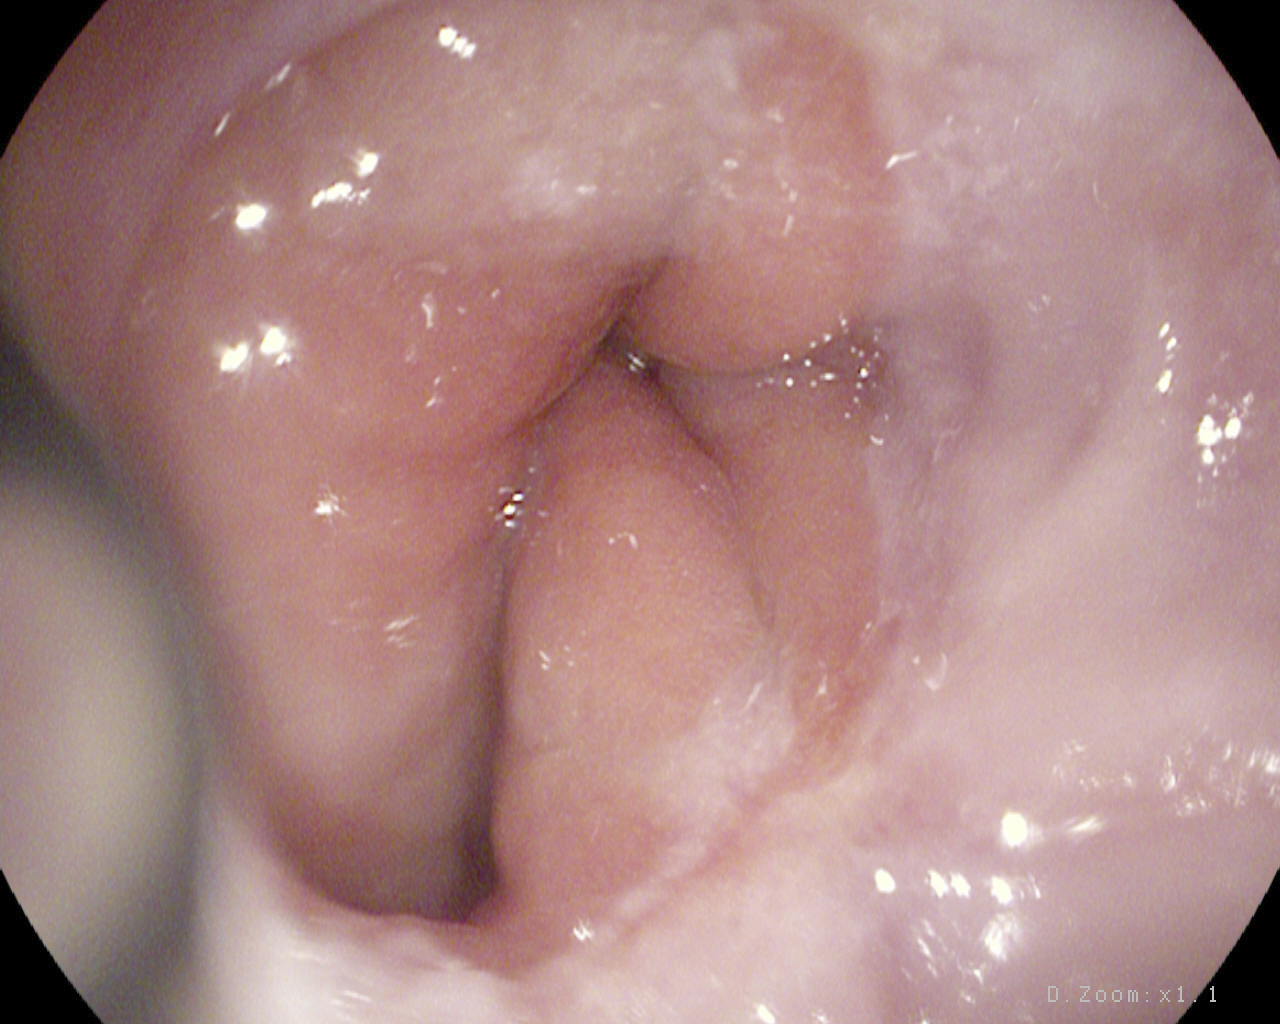
\includegraphics[height=\textwidth ,width=\textwidth]{experiments/figures/greensquare/zORIG.png}
            \caption{Original z-line image}    
            \label{fig:z_ORIG_SQUARE1}
        \end{subfigure}
        \qquad
        \begin{subfigure}[t]{\myfigsizethree}   
            \centering 
            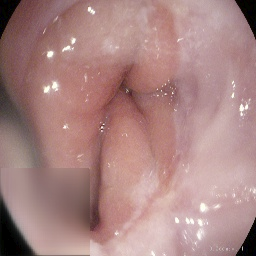
\includegraphics[width=\textwidth]{experiments/figures/greensquare/zAE.png}
            \caption{AE generated z-line image}    
            \label{fig:z_AE_SQUARE1}
        \end{subfigure}
        \qquad%\hfill%\quad
        \begin{subfigure}[t]{\myfigsizethree}   
            \centering 
            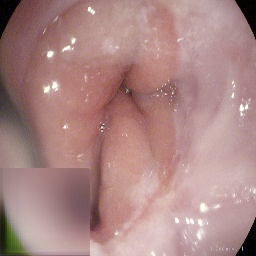
\includegraphics[width=\textwidth]{experiments/figures/greensquare/zGAN.png}
            \caption{GAN generated z-line image}    
            \label{fig:z_GAN_SQUARE1}
        \end{subfigure}
        \caption{Images from the polyp class and the normal-z-line class. Here we see results that needed finer detail when inpainting.} 
        \label{fig:AE_GAN_SQUARE1}
\end{figure}  
\begin{figure}
        %\centering
                \tiny
        \begin{subfigure}[t]{\myfigsizethree}
            \centering
            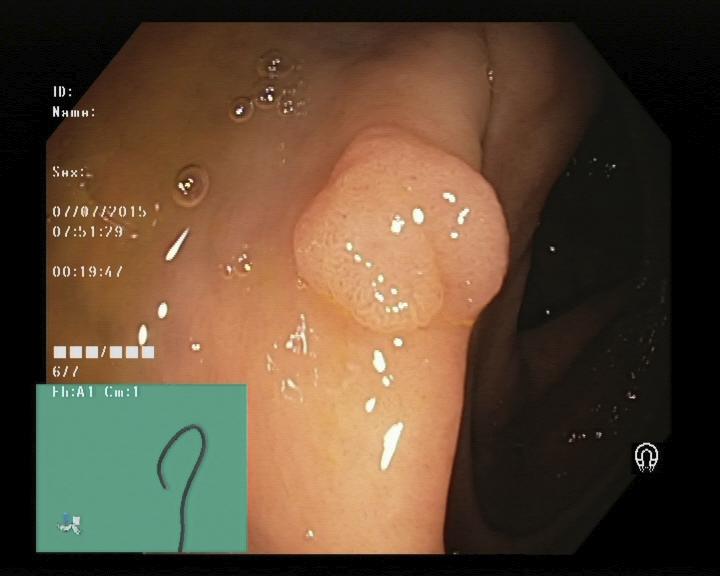
\includegraphics[height=\textwidth ,width=\textwidth]{experiments/figures/greensquare/normalmissORIG.png}
            \caption{Original polyp image}   
            \label{fig:polyp_ORIG_SQUARE2}
        \end{subfigure}
        \qquad
        \begin{subfigure}[t]{\myfigsizethree}
            \centering
            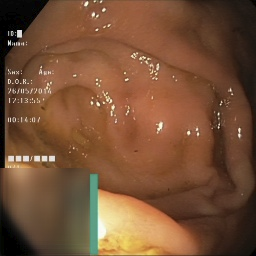
\includegraphics[width=\textwidth]{experiments/figures/greensquare/normalmissAE.png}
            \caption{AE generated polyp image }   
            \label{fig:polyp_AE_SQUARE2}
        \end{subfigure}
        \qquad
        \begin{subfigure}[t]{\myfigsizethree}  
            \centering 
            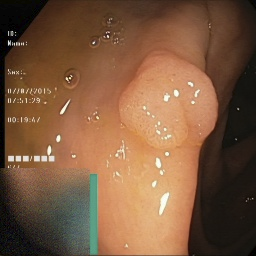
\includegraphics[width=\textwidth]{experiments/figures/greensquare/normalmissGAN.png}
            \caption{GAN generated plyp image}    
            \label{fig:polyp_GAN_SQUARE2}
        \end{subfigure}
        \qquad\vfill%\vskip\baselineskip
        \begin{subfigure}[t]{\myfigsizethree}   
            \centering 
            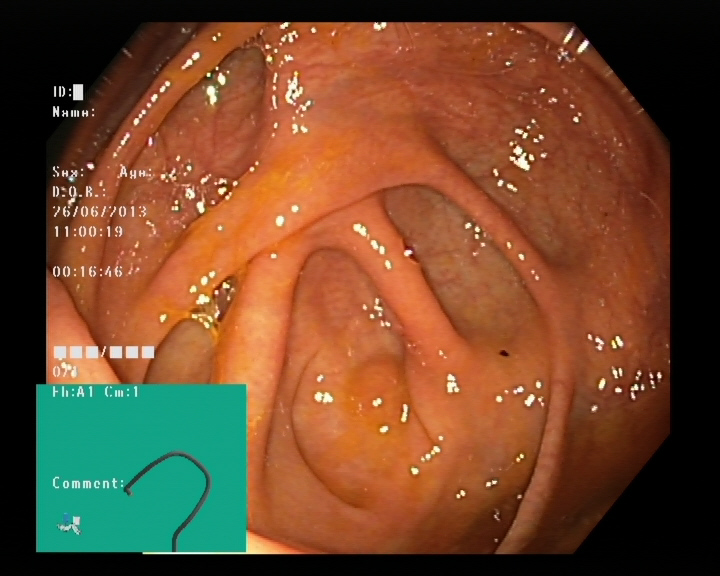
\includegraphics[height=\textwidth, width=\textwidth]{experiments/figures/greensquare/ncORIG.jpg}
            \caption{Original normal-cecum image}   
            \label{fig:nc_ORIG_SQUARE2}
        \end{subfigure}
        \qquad
        \begin{subfigure}[t]{\myfigsizethree}   
            \centering 
            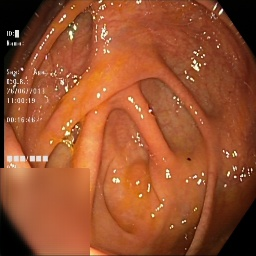
\includegraphics[width=\textwidth]{experiments/figures/greensquare/ncAE.jpg}
            \caption{AE generated normal-cecum image}   
            \label{fig:nc_AE_SQUARE2}
        \end{subfigure}
        \qquad%\hfill%\quad
        \begin{subfigure}[t]{\myfigsizethree}   
            \centering 
            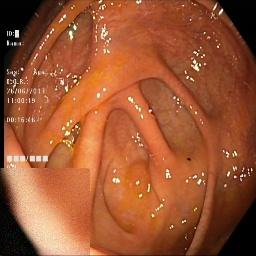
\includegraphics[width=\textwidth]{experiments/figures/greensquare/ncGAN.jpg}
            \caption{GAN generated normal-cecum image}  
            \label{fig:nc_GAN_SQUARE2}
        \end{subfigure}
        \caption{Images from the polyp class and the normal-cecum class. Here we have images with a problematic green square, and an image with details drawn from both sides of the inpainted area.} 
        \label{fig:AE_GAN_SQUARE2}
\end{figure}
    
Figure \ref{fig:AE_GAN_SQUARE1} and Figure \ref{fig:AE_GAN_SQUARE2} shows two examples from the datasets with the green square inpainted.
Figure \ref{fig:AE_GAN_SQUARE1} show images that, for both datasets, images are challenging areas to get correct, and require more than just colour matching to pass as real images. In the first image, a large part of a polyp is covered, and we can see that both algorithms try to recreate the area to varying success. We can see that the GAN is much better, in both examples, to find the right colours at the edges, giving a more natural look.
Another advantage with the GAN is the ability to estimate the corner size better, as we can see that the corner is unnaturally large in Figure \ref{fig:z_AE_SQUARE1} compared to Figure \ref{fig:z_GAN_SQUARE1}.
 
Figure \ref{fig:polyp_ORIG_SQUARE2},\ref{fig:polyp_AE_SQUARE2},\ref{fig:polyp_GAN_SQUARE2} shows how the two algorithms handles unexpected data. Here the green area was moved to the right to the point it was outside the mask range. Both algorithms added a green tint to the images, though the GAN did a better job making it natural looking. 
The last image set shows that the GAN has learned to connect structures throughout the inpainted area. The mucosa in Figure \ref{fig:nc_GAN_SQUARE2} the foreground is a full structure as we would expect if we removed the green square.
 


\vspace{5px}
\noindent Just as with the black corners, the training time for the AE regarding removing the green square took about 4 hours. 
The training time of the GAN was over two days, closer to three days. However, the ability to predict structures and overall a greater awareness of context might be worth the training time.

\FloatBarrier
\subsection{Combination}
The last two datasets (IV \& VII in Table \ref{tab:datasets}) were generated from the mask in Figure \ref{fig:BothMask}. The goal of the datasets generated by the AE and the GAN check how a combination of the previous datasets would do do to the classification. The same cropping-inpainting procedure were applied as with the other sets. The result is shown in Figure \ref{fig:AE_GAN_BOTH1} and Figure \ref{fig:AE_GAN_BOTH2}.

    
        \begin{figure}
        %\centering
        \tiny
		\begin{subfigure}[t]{\myfigsizethree}
            \centering
            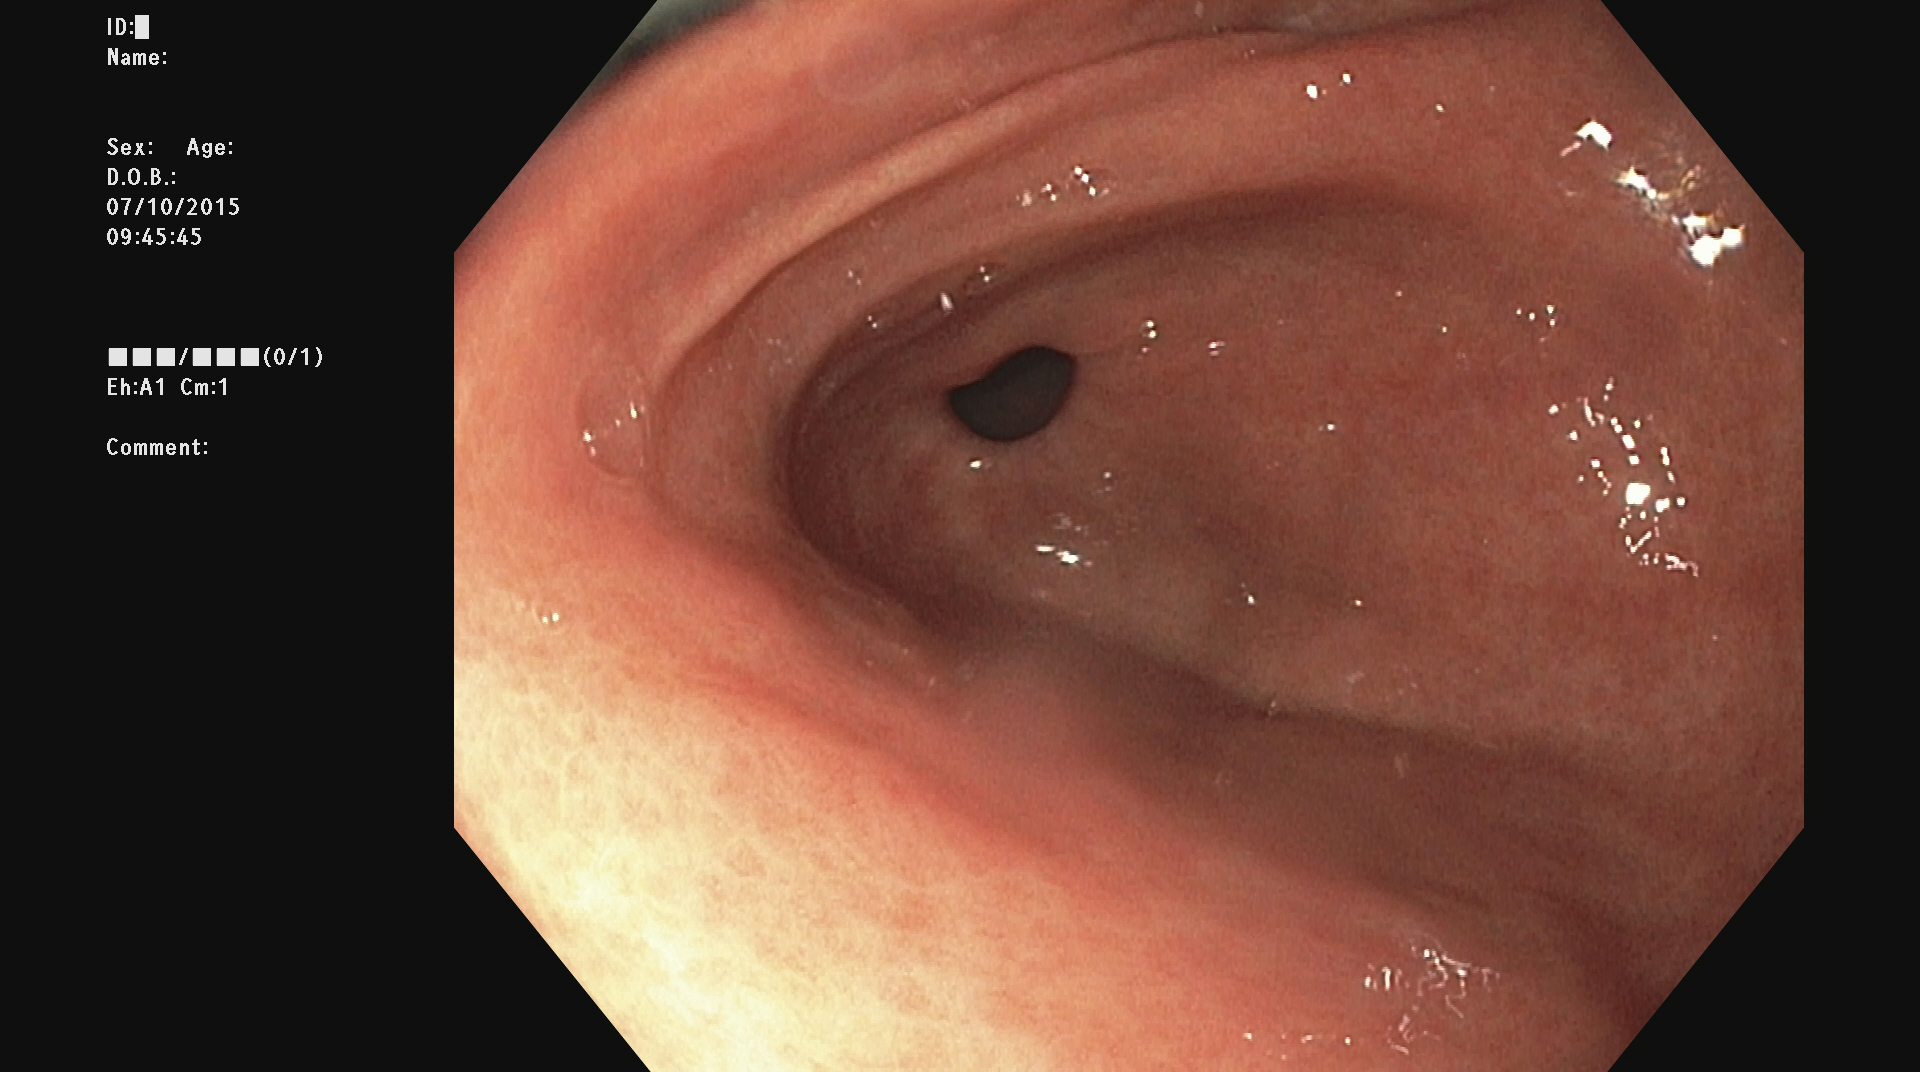
\includegraphics[height=\textwidth ,width=\textwidth]{experiments/figures/both/NPORIG.jpg}
            \caption{Original normal-pylorus image}    
            \label{fig:np_ORIG_both1}
        \end{subfigure}
        \qquad
        \begin{subfigure}[t]{\myfigsizethree}
            \centering
            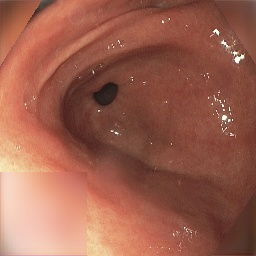
\includegraphics[width=\textwidth]{experiments/figures/both/NPAE.jpg}
            \caption{AE generated normal-pylorus image}    
            \label{fig:np_AE_both1}
        \end{subfigure}
        \qquad
        \begin{subfigure}[t]{\myfigsizethree}  
            \centering 
            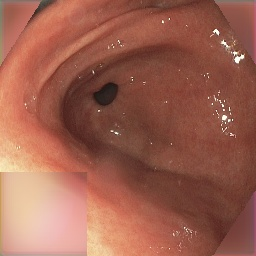
\includegraphics[width=\textwidth]{experiments/figures/both/NPGAN.jpg}
            \caption{GAN gnerated normal-pylorus image}    
            \label{fig:np_GAN_both1}
        \end{subfigure}
        \qquad\vfill%\vskip\baselineskip
        \begin{subfigure}[t]{\myfigsizethree}   
            \centering 
            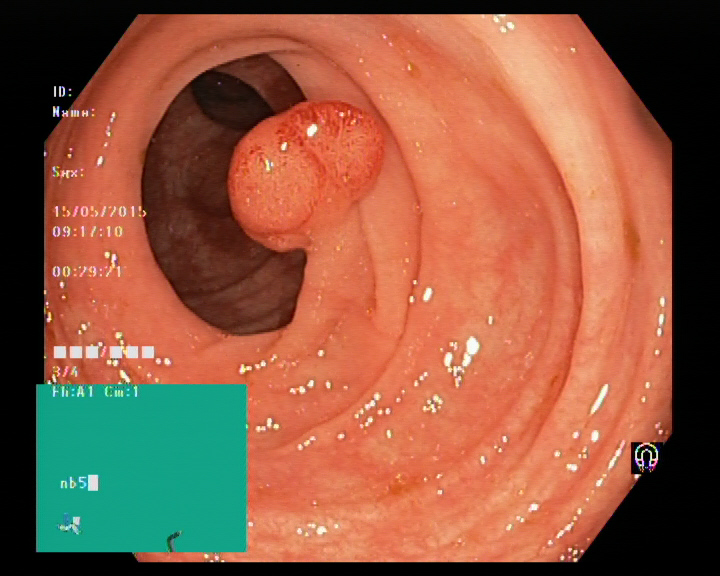
\includegraphics[height=\textwidth ,width=\textwidth]{experiments/figures/both/PORIG.jpg}
            \caption{Original polyp image}    
            \label{fig:p_ORIG_both1}
        \end{subfigure}
        \qquad
        \begin{subfigure}[t]{\myfigsizethree}   
            \centering 
            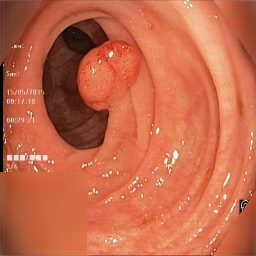
\includegraphics[width=\textwidth]{experiments/figures/both/PAE.jpg}
            \caption{AE generated polyp image}    
            \label{fig:p_AE_both1}
        \end{subfigure}
        \qquad%\hfill%\quad
        \begin{subfigure}[t]{\myfigsizethree}   
            \centering 
            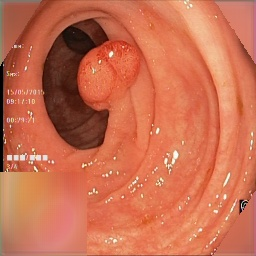
\includegraphics[width=\textwidth]{experiments/figures/both/PGAN.jpg}
            \caption{GAN generated polyp image}    
            \label{fig:p_GAN_both1}
        \end{subfigure}
        \caption{Images from the normal-pylorus an the polyp class. These images represent good images where most of the job was just to match the colour, rather than understanding complex structures in the images.} 
        \label{fig:AE_GAN_BOTH1}
    \end{figure}
    
    \begin{figure}
            \tiny
        %\centering
        \begin{subfigure}[t]{\myfigsizethree}
            \centering
            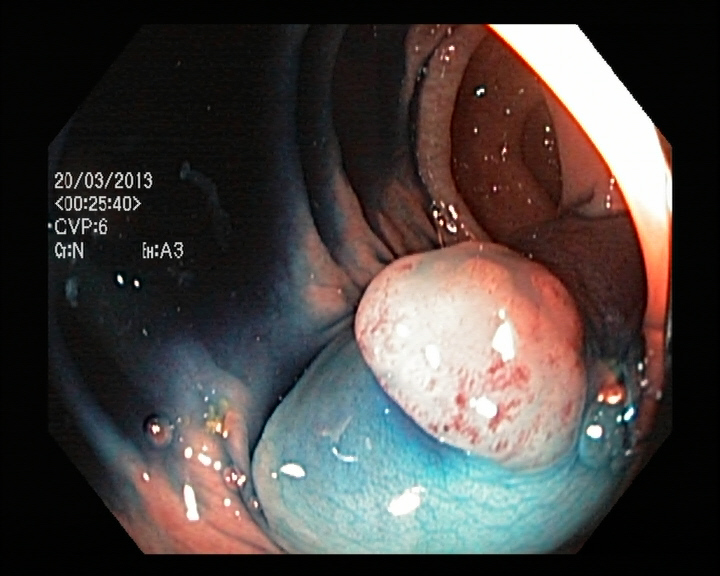
\includegraphics[height=\textwidth ,width=\textwidth]{experiments/figures/both/DLORIG.jpg}
            \caption{Original dye lifted polyp image}    
            \label{fig:dlp_ORIG_BOTH2}
        \end{subfigure}
        \qquad
        \begin{subfigure}[t]{\myfigsizethree}
            \centering
            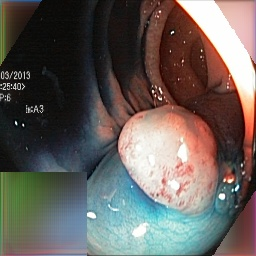
\includegraphics[width=\textwidth]{experiments/figures/both/DLAE.jpg}
            \caption{AE generated dye lifted polyp image}    
            \label{fig:dlp_AE_BOTH2}
        \end{subfigure}
        \qquad
        \begin{subfigure}[t]{\myfigsizethree}  
            \centering 
            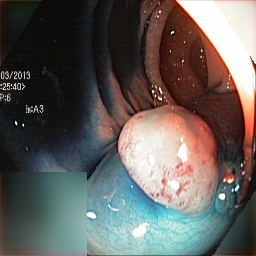
\includegraphics[width=\textwidth]{experiments/figures/both/DLGAN.jpg}
            \caption{GAN generated dye lifted polyp image}    
            \label{fig:dlp_GAN_BOTH2}
        \end{subfigure}
        \qquad\vfill%\vskip\baselineskip
		\begin{subfigure}[t]{\myfigsizethree}   
            \centering 
            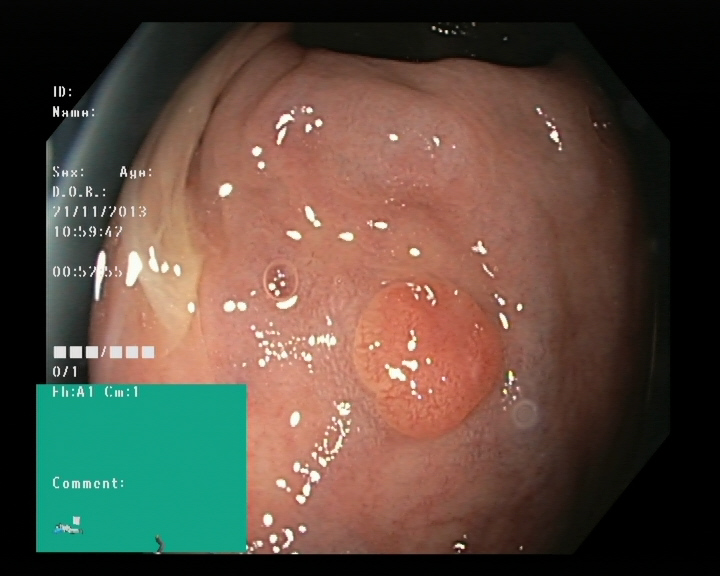
\includegraphics[height=\textwidth ,width=\textwidth]{experiments/figures/both/greenORIG.jpg}
            \caption{Original polyp image}    
            \label{fig:p_ORIG_BOTH2}
        \end{subfigure}
        \qquad
        \begin{subfigure}[t]{\myfigsizethree}   
            \centering 
            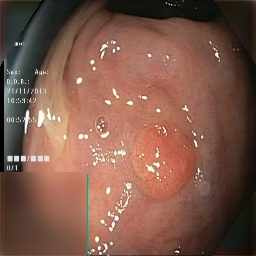
\includegraphics[width=\textwidth]{experiments/figures/both/greenAE.jpg}
            \caption{AE generated polyp image}    
            \label{fig:p_AE_BOTH2}
        \end{subfigure}
        \qquad%\hfill%\quad
        \begin{subfigure}[t]{\myfigsizethree}   
            \centering 
            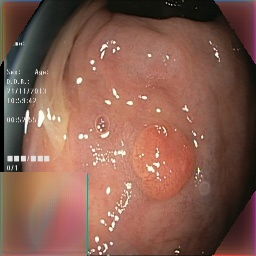
\includegraphics[width=\textwidth]{experiments/figures/both/greenGAN.jpg}
            \caption{GAN generated polyp image}    
            \label{fig:p_GAN_BOTH2}
        \end{subfigure}
        \caption{Images from the dye lifted polyp an the polyp class. The images were chosen because it highlighted flaws in both models. } 
        \label{fig:AE_GAN_BOTH2}
    \end{figure}

Figure \ref{fig:AE_GAN_BOTH1} and Figure \ref{fig:AE_GAN_BOTH2} shows two examples from the datasets with the green square inpainted as well as the black corners inpainted.
The first set of images in Figure \ref{fig:AE_GAN_BOTH1} shows cases where both algorithms did reasonably well. Here, most of the job was cutting the images, and because the areas inpainted were homogeneous, the main task was to colour-match the areas.

Figure \ref{fig:AE_GAN_BOTH2} show some more problematic areas. Image \ref{fig:dlp_AE_BOTH2} show a downfall with the AE by the fact that it uses a green colour not present in any of the training images. Luckily the GAN in Figure \ref{fig:dlp_GAN_BOTH2} manages to use the dyed mucosa to better inpaint the area.
We encounter the opposite problem in Figure \ref{fig:p_ORIG_BOTH2}, \ref{fig:p_AE_BOTH2} and \ref{fig:p_GAN_BOTH2}. Here the AE manages to not use the blue strip to inpaint the square green, while the GAN does. 
This mispainting by the GAN is probably caused by the blue ´´instrument'' in the top left corner of the image. Here we believe the GAN misclassifies the image, assuming it is a dyed-lifted-polyp, and subsequently fills in the blue ink into the image.


\vspace{5px}
\noindent The training time for the total AE inpainting was the longest, but still within 5 hours.
Just as with the inpainted corners, the training time of the GAN was closer to three days. The results were reasonably better. 


\subsection{Double resolution}
\todo{
Make shure 512 resolution is described proppery before table tab:datasets 
}

In addition to the datasets at standard size, we created the datasets at double resolution (IX \& XIV in Table \ref{tab:datasets}).  The goal of the seven datasets generated at double resolution was to see how image size affects the results. We apply the same cropping-inpainting procedure as with the other sets. The result is shown in Figure \ref{fig:AE_GAN_512}.

As we see in figure \ref{fig:AE_GAN_512} the inpainted areas is more smeared out in contrast to the previous datasets. In this thesis, we have chosen to keep our focus primarily on the images at $256\times 256$ px resolution though we keep the double resolution images as a means to draw more context from our results.


        \begin{figure}[t]
        %\centering
        \tiny
		\begin{subfigure}[t]{\myfigsizethree}
            \centering
            \includegraphics[height=\textwidth ,width=\textwidth]{experiments/figures/512/orig.jpg}
            \caption{Original esophagitis image}    
            \label{fig:ORIG_512}
        \end{subfigure}
        \qquad
        \begin{subfigure}[t]{\myfigsizethree}
            \centering
            \includegraphics[width=\textwidth]{experiments/figures/512/ae.jpg}
            \caption{AE generated esophagitis image}    
            \label{fig:AE_512}
        \end{subfigure}
        \qquad
        \begin{subfigure}[t]{\myfigsizethree}  
            \centering 
            \includegraphics[width=\textwidth]{experiments/figures/512/cc.jpg}
            \caption{GAN gnerated esophagitis image}    
            \label{fig:GAN_512}
        \end{subfigure}
        \caption{Images from the esophagitis class.The images from the double resolution dataset is much more smeared out compared to the smaller images.} 
        \label{fig:AE_GAN_512}
    \end{figure}



   
\FloatBarrier
\section{Results of the transfer learning experiments}In the previous section, we looked at the generation of the new datasets. We looked at how the different hypothesises formed the basis for different masking, and we discussed downfall and advantages with the autoencoder method versus the GAN method. 
We will now look at the results when using the newly created datasets when training a classifier for each one of them. 
The model used for the classifier is the same for all the datasets. We use the same learning rate, the same model, and the same parameters for early stopping of the training.  In this section we will first go through the model, then we will look at the results for each of the runs.


\subsection{Models}
The classification model is constructed to give the best real-world correspondence.

First, we supply info about the model. This information is for instance batch size, type of network, and choice of an optimiser. 
The transfer learning network chosen is loaded with the imagenet weights. With the model loaded into memory, the global average pooling layer is added, followed by a fully connected layer with the number of nodes equal to the number of classes in the input dataset and a softmax activation step as described in more detail in chapter \ref{cha:classifier}. 

With the model loaded we complete it by adding the desired optimiser, and set parameters like batch size, learning rate, validation patience, and image size.

As described, we increase our confidence in our results by using K-fold cross-validation. This method ensures a realistic result using the theoretically best model for the task. 
When we are looking at the models, we use the base case results as a reference point improve upon. This base case is the result of a standard run of classification without any inpainting.


\FloatBarrier
\section{Densenet121}

As stated in Section \ref{cha:classifier}, we use the research provided by Borgli et al. in hyperparameter optimisation~\cite{runeMedico2018}. We concluded that Densenet121 is the optimal network to achieve the highest score when both training and evaluating on the Kvasir dataset. 

Based on the results, we assume that Densenet121 will give the best results both when evaluating our network on the Kvasir dataset, and when we use the generalised models on the CVC datasets. The stats for the Densenet training routine is shown in Table \ref{tab:TrainingAttrDN121}.



\begin{table}[h]
\caption{Training attributes for Densenet121 base model }
\begin{center}
\begin{tabular}{ll}
\toprule
Atribute                & Value   \\
\midrule
Max Number of epochs    & 20      \\
Patience for validation & 3       \\
Folds                   & 6       \\
Image size              & 256x256 \\
Batch size              & 24      \\   
\bottomrule
\end{tabular}
\end{center}
\label{tab:TrainingAttrDN121}
\end{table}

The reasoning behind the training attributes for each of the parameters can be summarised with:

The max number of epochs is an artificial roof where we do not allow any more training, even when the network is improving.  We believe that the network, should it come to 20 epochs, will only overfit the results.
We have chosen training patience of three. This patience is a compromise between a higher value, more likely to overfit, and a lower value, more likely to stop too early to learn all the meaningful representations. 
In addition to the number of epochs trained we divided Kvasir into six folds. Based on the six folds we got 1333 images for both validation and testing, while the majority of the images would be used for training. A smaller fold would leave the training with too little data, and hence we could not expect as good of a result. A higher number of folds would increase the number of training runs substantially, since we are training on 14 datasets.
Finally, the batch size was decided to be the highest number that did not give any memory issues.  We believe that a batch size of 24 is well within the scope of reality.
\clearpage
\FloatBarrier
\subsection{Densenet121 Base Model}
We present the results from the Densenet121 network in table \ref{fig:results_DN121_base}.
This table shows the base case result with the Densenet121 model, meaning the unaugmented dataset. 

\begin{figure}[t]
%\caption{Densenet121 Base results}
\myfontsize
%\advance\leftskip-1.5cm
\caption*{\footnotesize \textmd{ \textbf{A}:{dyed-lifted-polyps} , \textbf{B}:{dyed-resection-margins} , \textbf{C}:{esophagitis} , \textbf{D}:{normal-cecum} , \textbf{E}:{normal-pylorus} , \textbf{F}:{normal-z-line} , \textbf{G}:{polyps} , \textbf{H}:{ulcerative-colitis} , \textbf{I}:{non-polyp}}}

\begin{subfigure}[b]{0.25\textwidth}
     
\[
\begin{blockarray}{ccc}
& I & G  \\
\begin{block}{c[cc]}
        I&1310 &  37\\
        G& 618 &  319\\
\end{block}
\end{blockarray}
 \]         

\caption{Baseline Confusion matrix for the CVC 356 dataset}
\label{mat:cvc356_CM_DN121_base}
\end{subfigure}
\begin{subfigure}[b]{0.49\textwidth}  
\scriptsize     
\[
\begin{blockarray}{ccccccccc}
& A & B & C & D & E & F & G & H \\
\begin{block}{c[cccccccc]}
A&150 & 6 & 0 & 0 & 0 & 0 & 1 & 0\\
B& 14 & 160 & 0 & 0 & 0 & 0 & 0 & 0\\
C&  0 & 0 & 130 & 0 & 1 & 19 & 0 & 0\\
D&  0 & 0 & 0 & 162 & 0 & 0 & 1 & 3\\
E&  0 & 0 & 0 & 0 & 164 & 0 & 0 & 0\\
F&  0 & 0 & 36 & 0 & 0 & 147 & 1 & 0\\
G&  1 & 0 & 0 & 3 & 1 & 0 & 161 & 2\\
H&  1 & 0 & 0 & 1 & 0 & 0 & 2 & 161\\
\end{block}
\end{blockarray}
 \]        
        
        
\caption{Baseline \\Confusion matrix for \\the Kvasir dataset}
\label{mat:kvasir_CM_DN121_base}
\end{subfigure}
\begin{subfigure}[b]{0.25\textwidth}
        \[
\begin{blockarray}{ccc}
& I & G  \\
\begin{block}{c[cc]}
 		I&1311 & 3553\\
        G&618  & 6472\\
\end{block}
\end{blockarray}
\]   
\caption{Baseline Confusion matrix for the CVC 12k dataset}
\label{mat:cvc12k_CM_DN121_base}
\end{subfigure}

\vspace{1cm}

%\caption{Confusion matrices for the three datasets}
%\label{mat:CM_DN121_base}
\begin{subfigure}[t]{0.25\textwidth}
\begin{tabular}{ll}      
        \toprule
        \multicolumn{2}{c}{CVC 356 dataset}        \\
        \midrule
        MCC 		& 0.4244 \\
        F1  		& 0.6467 \\
        Precicion  	& 0.7878 \\
        Recall     	& 0.6565 \\
        Accuracy	& 0.7132 \\
        \bottomrule
        \end{tabular}
\caption{The CVC 356 dataset Metrics}
\label{tab:cvc356_metrics_DN121_base}
\end{subfigure}%
\begin{subfigure}[t]{0.49\textwidth}
    	\centering
        \begin{tabular}{ll}
        \toprule
        \multicolumn{2}{c}{Kvasir dataset}        \\
        \midrule
        MCC 		& 0.9202 \\
        F1  		& 0.9299 \\
        Precicion  	& 0.93 \\
        Recall     	& 0.9313  \\
        Accuracy	& 0.93 \\
        
        \bottomrule
\end{tabular}
\caption{The Kvasir dataset\\ Metrics}
\label{tab:kvasir_metrics_DN121_base}
\end{subfigure}%
\begin{subfigure}[t]{0.25\textwidth}
        \begin{tabular}{ll}
        \toprule
        \multicolumn{2}{c}{CVC 12k dataset}        \\
        \midrule
        MCC 		& 0.2435  \\
        F1  		& 0.5711 \\
        Precicion  	& 0.6626 \\
        Recall     	& 0.5912 \\
        Accuracy	& 0.6511 \\
        \bottomrule
        \end{tabular}
\caption{The CVC 12k dataset Metrics}
\label{tab:cvc12k_metrics_DN121_base}
\end{subfigure}
%\caption{The baseline confusion matrixes}
\caption{Densenet121 Base results}
\label{fig:results_DN121_base}
%\advance\rightskip-1.5cm
\end{figure}



\noindent
The Matrices in Figure \ref{fig:results_DN121_base} shows the evaluation of the test set on each of the three datasets used. 

On the Kvasir dataset, we used five folds for training and validation, and the last sixth fold for the testing. That left us with 1342 images divided evenly between the classes. The CVC datasets were only used for testing and hence did not need k fold cross-validation.

\paragraph{CVC 356}
The CVC 356 base case MCC lies at 0.42 with an accuracy of 71\%. 
From the Confusion matrix, we can discern that most polyps were classified correctly, except for 37 polyp images incorrectly classified as non-polyp. Moreover, we also had 618 cases of non-polyps classified as polyps.
In a vacuum, the results are adequate, showing a high accuracy on an unseen dataset.

\paragraph{The Kvasir}
In this Confusion matrix, we see that most of the samples lie throughout the diagonal, which, as we recall, is the correct classification. 
The Kvasir base case MCC lies at 0.92 which coincides with a near perfect accuracy given the complexity of the dataset. 
The misclassification is between the esophagitis class, and the normal-z-line class, which are already two notoriously different classes to differentiate.
There is also a small mixup between dyed lifted polyps and dyed resection margins, another remarkably different classification task. 


\paragraph{CVC 12k}
The CVC 12k base case MCC lies at 0.24 with an accuracy of 65\%. 
From the Confusion matrix, we can discern that most polyps were classified correctly, though the model missed a third of the polyps.
Though the accuracy were 65\%, this model most likely did not learn the essential features for classifying polyps.



\FloatBarrier
\clearpage
\subsection{Densenet121 Corners Inpainted}
Based on Hypothesis \ref{hyp:a} we would expect the act of inpainting the corner in the images to give Kvasir a higher score compared to the baseline. Also, we should see improvement in both CVC 356 and CVC 12k.
We present the dataset created by the  GAN followed by the dataset created by the Autoencoder evaluated with the Densenet121 model.

\begin{figure}
%\caption{Densenet121 Inpainted corners with the GAN results}
\myfontsize
%\advance\leftskip-1.5cm
\caption*{\footnotesize \textmd{ \textbf{A}:{dyed-lifted-polyps} , \textbf{B}:{dyed-resection-margins} , \textbf{C}:{esophagitis} , \textbf{D}:{normal-cecum} , \textbf{E}:{normal-pylorus} , \textbf{F}:{normal-z-line} , \textbf{G}:{polyps} , \textbf{H}:{ulcerative-colitis} , \textbf{I}:{non-polyp}}}

\begin{subfigure}[b]{0.25\textwidth}
     
\[
\begin{blockarray}{ccc}
& I & G  \\
\begin{block}{c[cc]}
        I&1647 &  179\\
        G& 281 &  177\\
\end{block}
\end{blockarray}
 \]         

\caption{GAN corners Confusion matrix for the CVC 356 dataset}
\label{mat:cvc356_CM_DN121_GAN_CORNER}
\end{subfigure}
\begin{subfigure}[b]{0.49\textwidth}  
\scriptsize     
\[
\begin{blockarray}{ccccccccc}
& A & B & C & D & E & F & G & H \\
\begin{block}{c[cccccccc]}
A&157 & 12 & 0 & 0 & 0 & 0 & 0 & 0\\
B&  8 & 154 & 0 & 0 & 0 & 0 & 0 & 0\\
C&  0 & 0 & 116 & 0 & 0 & 11 & 0 & 0\\
D&  0 & 0 & 0 & 162 & 0 & 0 & 3 & 5\\
E&  0 & 0 & 1 & 0 & 166 & 0 & 3 & 0\\
F&  0 & 0 & 49 & 0 & 0 & 155 & 1 & 0\\
G&  1 & 0 & 0 & 2 & 0 & 0 & 158 & 2\\
H&  0 & 0 & 0 & 2 & 0 & 0 & 1 & 159\\
\end{block}
\end{blockarray}
 \]        
        
        
\caption{GAN corners \\Confusion  matrix for \\the Kvasir dataset}
\label{mat:kvasir_CM_DN121_GAN_CORNER}
\end{subfigure}
\begin{subfigure}[b]{0.25\textwidth}
        \[
\begin{blockarray}{ccc}
& I & G  \\
\begin{block}{c[cc]}
 		I&1648 & 4699\\
        G&281  & 5326\\
\end{block}
\end{blockarray}
\]   
\caption{GAN corners Confusion matrix for the CVC 12k dataset}
\label{mat:cvc12k_CM_DN121_GAN_CORNER}
\end{subfigure}

\vspace{1cm}

%\caption{Confusion matrices for the three datasets}
\label{mat:CM_DN121_GAN_CORNER}
\begin{subfigure}[t]{0.25\textwidth}
\begin{tabular}{ll}      
        \toprule
        \multicolumn{2}{c}{CVC 356 dataset}        \\
        \midrule
        MCC 		& 0.3184 \\
        F1  		& 0.6562 \\
        Precicion  	& 0.6757 \\
        Recall     	& 0.6442 \\
        Accuracy	& 0.7986 \\
        \bottomrule
        \end{tabular}
\caption{The CVC 356 dataset Metrics}
\label{tab:cvc356_metrics_DN121_GAN_CORNER}
\end{subfigure}%
\begin{subfigure}[t]{0.49\textwidth}
    	\centering
        \begin{tabular}{ll}
        \toprule
        \multicolumn{2}{c}{Kvasir dataset}        \\
        \midrule
        MCC 		& 0.914 \\
        F1  		& 0.9233 \\
        Precicion  	& 0.9239 \\
        Recall     	& 0.9287 \\
        Accuracy	& 0.9239 \\
        \bottomrule
\end{tabular}
\caption{The Kvasir dataset\\ Metrics}
\label{tab:kvasir_metrics_DN121_GAN_CORNER}
\end{subfigure}%
\begin{subfigure}[t]{0.25\textwidth}
        \begin{tabular}{ll}
        \toprule
        \multicolumn{2}{c}{CVC 12k dataset}        \\
        \midrule
        MCC 		& 0.2842 \\
        F1  		& 0.5398 \\
        Precicion  	& 0.6928 \\
        Recall     	& 0.6048 \\
        Accuracy	& 0.5834 \\
        \bottomrule
        \end{tabular}
\caption{The CVC 12k dataset Metrics}
\label{tab:cvc12k_metrics_DN121_GAN_CORNER}
\end{subfigure}
\caption{Densenet121 Inpainted corners with the GAN results}
\label{fig:results_DN121_GAN_CORNER}
%\caption{The inpainted corner with GAN confusion matrixes}
%\advance\rightskip-1.5cm
\end{figure}
\FloatBarrier



\begin{figure}
%\caption{Densenet121 Inpainted corners with the AE results}
\myfontsize
%\advance\leftskip-1.5cm
\caption*{\footnotesize \textmd{ \textbf{A}:{dyed-lifted-polyps} , \textbf{B}:{dyed-resection-margins} , \textbf{C}:{esophagitis} , \textbf{D}:{normal-cecum} , \textbf{E}:{normal-pylorus} , \textbf{F}:{normal-z-line} , \textbf{G}:{polyps} , \textbf{H}:{ulcerative-colitis} , \textbf{I}:{non-polyp}}}

\begin{subfigure}[b]{0.25\textwidth}
     
\[
\begin{blockarray}{ccc}
& I & G  \\
\begin{block}{c[cc]}
        I&1746 & 106\\
        G&  182 & 250\\
\end{block}
\end{blockarray}
 \]         

\caption{AE corners Confusion matrix for the CVC 356 dataset}
\label{mat:cvc356_CM_DN121_AE_CORNER}
\end{subfigure}
\begin{subfigure}[b]{0.49\textwidth}  
\scriptsize     
\[
\begin{blockarray}{ccccccccc}
& A & B & C & D & E & F & G & H \\
\begin{block}{c[cccccccc]}
A&150 & 9 & 0 & 0 & 0 & 0 & 1 & 0\\
B& 12 & 157 & 0 & 0 & 0 & 0 & 0 & 0\\
C&  0 & 0 & 141 & 0 & 0 & 21 & 0 & 0\\
D&  1 & 0 & 0 & 160 & 0 & 0 & 4 & 2\\
E&  0 & 0 & 0 & 0 & 166 & 0 & 1 & 0\\
F&  0 & 0 & 25 & 0 & 0 & 145 & 0 & 0\\
G&  3 & 0 & 0 & 3 & 0 & 0 & 157 & 2\\
H&  0 & 0 & 0 & 3 & 0 & 0 & 3 & 162\\
\end{block}
\end{blockarray}
 \]        
        
        
\caption{AE corners \\Confusion matrix for\\ the Kvasir dataset}
\label{mat:kvasir_CM_DN121_AE_CORNER}
\end{subfigure}
\begin{subfigure}[b]{0.25\textwidth}
        \[
\begin{blockarray}{ccc}
& I & G  \\
\begin{block}{c[cc]}
 		I&1747 & 5227\\
        G&182  & 4798\\
\end{block}
\end{blockarray}
\]   
\caption{AE corners \\Confusion matrix for\\ the CVC 12k dataset}
\label{mat:cvc12k_CM_DN121_AE_CORNER}
\end{subfigure}

\vspace{1cm}

%\caption{Confusion matrices for the three datasets}
%\label{mat:CM_DN121_AE_CORNER}
\begin{subfigure}[t]{0.25\textwidth}
\begin{tabular}{ll}      
        \toprule
        \multicolumn{2}{c}{CVC 356 dataset}        \\
        \midrule
        MCC 		& 0.563 \\
        F1  		& 0.7792 \\
        Precicion  	& 0.8039 \\
        Recall     	& 0.7607 \\
        Accuracy	& 0.8739 \\
        \bottomrule
        \end{tabular}
\caption{The CVC 356 dataset Metrics}
\label{tab:cvc356_metrics_DN121_AE_CORNER}
\end{subfigure}%
\begin{subfigure}[t]{0.49\textwidth}
    	\centering
        \begin{tabular}{ll}
        \toprule
        \multicolumn{2}{c}{Kvasir dataset}        \\
        \midrule
        MCC 		& 0.9226 \\
        F1  		& 0.9321 \\
        Precicion  	& 0.9322 \\
        Recall     	& 0.9322 \\
        Accuracy	& 0.9322 \\
        \bottomrule
\end{tabular}
\caption{The Kvasir dataset\\ Metrics}
\label{tab:kvasir_metrics_DN121_AE_CORNER}
\end{subfigure}%
\begin{subfigure}[t]{0.25\textwidth}
        \begin{tabular}{ll}
        \toprule
        \multicolumn{2}{c}{CVC 12k dataset}        \\
        \midrule
        MCC 		& 0.2867 \\
        F1  		& 0.516  \\
        Precicion  	& 0.6921 \\
        Recall     	& 0.607 \\
        Accuracy	& 0.5475 \\
        \bottomrule
        \end{tabular}
\caption{The CVC 12k dataset Metrics}
\label{tab:cvc12k_metrics_DN121_AE_CORNER}
\end{subfigure}
%\caption{The inpainted corner with AE confusion matrixes}
\caption{Densenet121 Inpainted corners with the AE results}
\label{fig:results_DN121_AE_CORNER}
%\advance\rightskip-1.5cm
\end{figure}


%
\noindent Figure \ref{fig:results_DN121_GAN_CORNER} and \ref{fig:results_DN121_AE_CORNER} shows the evaluation of the test set on each of the three datasets made by both the Autoencoder and GAN. 

\paragraph{CVC 356}
We got the highest MCC from the Autoencoder with a score of 0.56 compared to a score of 0.31 from the GAN.
In general, the Autoencoder has a higher score overall compared to the GAN, where the Autoencoder reaches a higher score than the base case, and the GAN does not.
This difference indicates that the way the Autoencoder inpaints sparsly covered areas gives an edge in this use case. 


\paragraph{The Kvasir}
When evaluating our results on the Kvasir dataset we see similar scores for both the GAN and Autoencoder with 0.91 and 0.92 respectively. Here the Autoencoder reaches a higher score than the base case, though the margin is too small to significant.
We can discern that the number of small errors throughout the confusion matrices increases, indicating that the inpainted areas negatively help with classification.

\paragraph{CVC 12k}
The MCC scores for the GAN and Autoencoder both reaches a higher value than the base case. When inpainting the corners we see an increase in MCC value of 0.04 for both methods, giving some indication that removing areas with sparse information might give a higher classification score on other datasets with the same sparse areas.






































\FloatBarrier
\clearpage
\subsection{Densenet121 Green Square Inpainted}


We can recall from Hypothesis \ref{hyp:b} that removing dataset specific artefacts we will achieve a higher classification score when evaluating our models on previously unseen datasets.
In this experiment, we expect the Kvasir dataset not show any improvements, though both the CVC 356 and the CVC 12k dataset we hope to improve compared to the base case. 
We present the dataset created by the GAN followed by the dataset created by the Autoencoder and evaluate their performance with the Densenet model together.


\begin{figure}[t]
%\caption{Densenet121 Inpainted green square with the GAN results}
\myfontsize
%\advance\leftskip-1.5cm
\caption*{\footnotesize \textmd{ \textbf{A}:{dyed-lifted-polyps} , \textbf{B}:{dyed-resection-margins} , \textbf{C}:{esophagitis} , \textbf{D}:{normal-cecum} , \textbf{E}:{normal-pylorus} , \textbf{F}:{normal-z-line} , \textbf{G}:{polyps} , \textbf{H}:{ulcerative-colitis} , \textbf{I}:{non-polyp}}}

\begin{subfigure}[b]{0.25\textwidth}
     
\[
\begin{blockarray}{ccc}
& I & G  \\
\begin{block}{c[cc]}
        I&1848 &  92\\
        G& 80 &  264\\
\end{block}
\end{blockarray}
 \]         

\caption{GAN green square Confusion matrix for the CVC 356 dataset}
\label{mat:cvc356_CM_DN121_GAN_SQUARE}
\end{subfigure}
\begin{subfigure}[b]{0.49\textwidth}  
\scriptsize     
\[
\begin{blockarray}{ccccccccc}
& A & B & C & D & E & F & G & H \\
\begin{block}{c[cccccccc]}
A&157 & 13 & 0 & 0 & 0 & 0 & 0 & 0\\
B&  7 & 153 & 0 & 0 & 0 & 0 & 0 & 0\\
C&  0 & 0 & 146 & 0 & 1 & 37 & 0 & 0\\
D&  0 & 0 & 0 & 161 & 0 & 0 & 8 & 4\\
E&  0 & 0 & 1 & 0 & 165 & 1 & 1 & 0\\
F&  0 & 0 & 19 & 0 & 0 & 128 & 0 & 0\\
G&  2 & 0 & 0 & 3 & 0 & 0 & 153 & 0\\
H&  0 & 0 & 0 & 2 & 0 & 0 & 4 & 162\\
\end{block}
\end{blockarray}
 \]        
        
        
\caption{GAN green square\\ Confusion matrix for \\the Kvasir dataset}
\label{mat:kvasir_CM_DN121_GAN_SQUARE}
\end{subfigure}
\begin{subfigure}[b]{0.25\textwidth}
        \[
\begin{blockarray}{ccc}
& I & G  \\
\begin{block}{c[cc]}
 		I&1849 & 6850\\
        G&  80 & 3175\\
\end{block}
\end{blockarray}
\]   
\caption{GAN green square Confusion matrix for the CVC 12k dataset}
\label{mat:cvc12k_CM_DN121_GAN_SQUARE}
\end{subfigure}

\vspace{1cm}

%\caption{Confusion matrices for the three datasets}
%\label{mat:CM_DN121_GAN_SQUARE}
\begin{subfigure}[t]{0.25\textwidth}
\begin{tabular}{ll}      
        \toprule
        \multicolumn{2}{c}{CVC 356 dataset}        \\
        \midrule
        MCC 		& 0.71 \\
        F1  		& 0.8549 \\
        Precicion  	& 0.85 \\
        Recall     	& 0.86 \\
        Accuracy	& 0.9247  \\         
        \bottomrule
        \end{tabular}
\caption{The CVC 356 dataset Metrics}
\label{tab:cvc356_metrics_DN121_GAN_SQUARE}
\end{subfigure}%
\begin{subfigure}[t]{0.49\textwidth}
    	\centering
        \begin{tabular}{ll}
        \toprule
        \multicolumn{2}{c}{Kvasir dataset}        \\
        \midrule
        MCC 		& 0.9116 \\
        F1  		& 0.9222  \\
        Precicion  	& 0.9224 \\
        Recall     	& 0.9237 \\
        Accuracy	& 0.9224 \\
        \bottomrule
\end{tabular}
\caption{The Kvasir dataset\\ Metrics}
\label{tab:kvasir_metrics_DN121_GAN_SQUARE}
\end{subfigure}%
\begin{subfigure}[t]{0.25\textwidth}
        \begin{tabular}{ll}
        \toprule
        \multicolumn{2}{c}{CVC 12k dataset}        \\
        \midrule
        MCC 		& 0.2275 \\
        F1  		& 0.4131 \\
        Precicion  	& 0.6376 \\
        Recall     	& 0.594 \\
        Accuracy	& 0.4203 \\
        \bottomrule
        \end{tabular}
\caption{The CVC 12k dataset Metrics}
\label{tab:cvc12k_metrics_DN121_GAN_SQUARE}
\end{subfigure}
%\caption{The inpainted green square with GAN confusion matrixes}
\caption{Densenet121 Inpainted green square with the GAN results}
\label{fig:results_DN121_GAN_SQUARE}
%\advance\rightskip-1.5cm
\end{figure}
\FloatBarrier



\begin{figure}[t]
%\caption{Densenet121 Inpainted green square with the AE results}
\myfontsize
%\advance\leftskip-1.5cm
\caption*{\footnotesize \textmd{ \textbf{A}:{dyed-lifted-polyps} , \textbf{B}:{dyed-resection-margins} , \textbf{C}:{esophagitis} , \textbf{D}:{normal-cecum} , \textbf{E}:{normal-pylorus} , \textbf{F}:{normal-z-line} , \textbf{G}:{polyps} , \textbf{H}:{ulcerative-colitis} , \textbf{I}:{non-polyp}}}

\begin{subfigure}[b]{0.25\textwidth}
     
\[
\begin{blockarray}{ccc}
& I & G  \\
\begin{block}{c[cc]}
        I&1746 & 106\\
        G&  182 & 250\\
\end{block}
\end{blockarray}
 \]         

\caption{AE green square Confusion matrix for the CVC 356 dataset}
\label{mat:cvc356_CM_DN121_AE_SQUARE}
\end{subfigure}
\begin{subfigure}[b]{0.49\textwidth}  
\scriptsize     
\[
\begin{blockarray}{ccccccccc}
& A & B & C & D & E & F & G & H \\
\begin{block}{c[cccccccc]}
A&150 & 9 & 0 & 0 & 0 & 0 & 1 & 0\\
B& 12 & 157 & 0 & 0 & 0 & 0 & 0 & 0\\
C&  0 & 0 & 141 & 0 & 0 & 21 & 0 & 0\\
D&  1 & 0 & 0 & 160 & 0 & 0 & 4 & 2\\
E&  0 & 0 & 0 & 0 & 166 & 0 & 1 & 0\\
F&  0 & 0 & 25 & 0 & 0 & 145 & 0 & 0\\
G&  3 & 0 & 0 & 3 & 0 & 0 & 157 & 2\\
H&  0 & 0 & 0 & 3 & 0 & 0 & 3 & 162\\
\end{block}
\end{blockarray}
 \]        
        
        
\caption{AE green square\\ Confusion matrix for\\ the Kvasir dataset}
\label{mat:kvasir_CM_DN121_AE_SQUARE}
\end{subfigure}
\begin{subfigure}[b]{0.25\textwidth}
        \[
\begin{blockarray}{ccc}
& I & G  \\
\begin{block}{c[cc]}
 		I&1747 & 5227\\
        G&182  & 4798\\
\end{block}
\end{blockarray}
\]   
\caption{AE green square Confusion matrix for the CVC 12k dataset}
\label{mat:cvc12k_CM_DN121_AE_SQUARE}
\end{subfigure}

\vspace{1cm}

%\caption{Confusion matrices for the three datasets}
%\label{mat:CM_DN121_AE_SQUARE}
\begin{subfigure}[t]{0.25\textwidth}
\begin{tabular}{ll}      
        \toprule
        \multicolumn{2}{c}{CVC 356 dataset}        \\
        \midrule
        MCC 		& 0.6072 \\
        F1  		& 0.8017 \\
        Precicion  	& 0.8248 \\
        Recall      & 0.7837 \\
        Accuracy	& 0.8879 \\
        \bottomrule
            
        \end{tabular}
\caption{The CVC 356 dataset Metrics}
\label{tab:cvc356_metrics_DN121_AE_SQUARE}
\end{subfigure}%
\begin{subfigure}[t]{0.49\textwidth}
    	\centering
        \begin{tabular}{ll}
        \toprule
        \multicolumn{2}{c}{Kvasir dataset}        \\
        \midrule
        MCC 		& 0.9158 \\
        F1  		& 0.9262  \\
        Precicion  	& 0.9262 \\
        Recall     	& 0.9271  \\
        Accuracy	& 0.9262 \\
        \bottomrule
\end{tabular}
\caption{The Kvasir dataset\\ Metrics}
\label{tab:kvasir_metrics_DN121_AE_SQUARE}
\end{subfigure}%
\begin{subfigure}[t]{0.25\textwidth}
        \begin{tabular}{ll}
        \toprule
        \multicolumn{2}{c}{CVC 12k dataset}        \\
        \midrule
        MCC 		& 0.2029 \\
        F1  		& 0.4185  \\
        Precicion  	& 0.6257 \\
        Recall     	& 0.5819 \\
        Accuracy	& 0.4287 \\
        \bottomrule
        \end{tabular}
\caption{The CVC 12k dataset Metrics}
\label{tab:cvc12k_metrics_DN121_AE_SQUARE}
\end{subfigure}
%\caption{The inpainted green square with AE confusion matrixes}
\caption{Densenet121 Inpainted green square with the AE results}
\label{fig:results_DN121_AE_SQUARE}
%\advance\rightskip-1.5cm
\end{figure}

\noindent Figure \ref{fig:results_DN121_GAN_SQUARE} and \ref{fig:results_DN121_AE_SQUARE} shows the evaluation of the test set on each of the three datasets used both for the GAN and Autoencoder. 

\paragraph{CVC 356}
As this is a dataset unseen by the classifier during training, we would expect, given that Hypothesis \ref{hyp:b} is True, that the classification score would be higher than the base case.
Here we have \textit{significantly} higher score with both the GAN and Autoencoder. 
The GAN reached an MCC score of 0.71 compared to the base case of 42. The Autoencoder also beat the base case with a large margin, given the MCC score of 0.60. 
For both models, we see an increase in the recall, suggesting the number of mismatches decreased.

The results highly suggest that our hypothesis about removing dataset-specific artefacts to improve accuracy is indeed correct. 

\paragraph{The Kvasir}
As with the previous tests we see little change in the scores when evaluated on the Kvasir dataset.
Here both the GAN and the Autoencoder got a lower score compared to the base, though only with a small margin. Just like with the experiment with the corners inpainted, inpainting the green square does little to nothing with classification when the classifier already overfits.


\paragraph{CVC 12k}
As with the CVC 356 dataset, the CVC 12k dataset is unseen by the classifier during training. 
Here, both the GAN and Autoencoder reaches a lower MCC value when evaluated on the dataset. 
This result is a direct contradiction to the hypothesis \ref{hyp:b}, showing that removing dataset specific artefacts does not always yield better scores. 
It is important to note that there are significant differences between the two CVC datasets which can influence the results. The most prominent feature is the edges around the images in the 12k dataset. The much larger frames could  ´´overwrite'' much of the work done by inpainting the green square, and could subsequently disrupt the classifier.














































\FloatBarrier
\clearpage
\subsection{Densenet121 Full Inpainting}

In addition to testing the two hypothesises separately we, as we recall, want to check both types of inpainting at the same time.
When testing both inpainting types, we do not draw any predictions, given that we do not know if the two methods interfere with each other. 

We present the GAN inpainting of both the areas followed by the same inpainting with the Autoencoder.


\begin{figure}[t]
%\caption{Densenet121 Inpainted both areas with the GAN results}
\myfontsize
%\advance\leftskip-1.5cm
\caption*{\footnotesize \textmd{ \textbf{A}:{dyed-lifted-polyps} , \textbf{B}:{dyed-resection-margins} , \textbf{C}:{esophagitis} , \textbf{D}:{normal-cecum} , \textbf{E}:{normal-pylorus} , \textbf{F}:{normal-z-line} , \textbf{G}:{polyps} , \textbf{H}:{ulcerative-colitis} , \textbf{I}:{non-polyp}}}

\begin{subfigure}[b]{0.25\textwidth}
     
\[
\begin{blockarray}{ccc}
& I & G  \\
\begin{block}{c[cc]}
        I&1916 &  129\\
        G& 12 &  227\\
\end{block}
\end{blockarray}
 \]         

\caption{GAN both areas Confusion matrix for the CVC 356 dataset}
\label{mat:cvc356_CM_DN121_GAN_BOTH}
\end{subfigure}
\begin{subfigure}[b]{0.49\textwidth}  
\scriptsize     
\[
\begin{blockarray}{ccccccccc}
& A & B & C & D & E & F & G & H \\
\begin{block}{c[cccccccc]}
A&159 & 7 & 0 & 0 & 0 & 0 & 2 & 1\\
B&  7 & 158 & 0 & 0 & 0 & 0 & 0 & 0\\
C&  0 & 0 & 118 & 0 & 0 & 8 & 0 & 0\\
D&  0 & 0 & 0 & 161 & 0 & 0 & 3 & 4\\
E&  0 & 0 & 1 & 0 & 164 & 0 & 3 & 0\\
F&  0 & 0 & 47 & 0 & 0 & 158 & 1 & 0\\
G&  0 & 0 & 0 & 0 & 1 & 0 & 154 & 0\\
H&  0 & 1 & 0 & 5 & 1 & 0 & 3 & 161\\
\end{block}
\end{blockarray}
 \]        
        
        
\caption{GAN both areas \\Confusion matrix for \\the Kvasir dataset}
\label{mat:kvasir_CM_DN121_GAN_BOTH}
\end{subfigure}
\begin{subfigure}[b]{0.25\textwidth}
        \[
\begin{blockarray}{ccc}
& I & G  \\
\begin{block}{c[cc]}
 		I&1917 & 7851\\
        G&  12 & 2174\\
\end{block}
\end{blockarray}
\]   
\caption{GAN both areas Confusion matrix for the CVC 12k dataset}
\label{mat:cvc12k_CM_DN121_GAN_BOTH}
\end{subfigure}
%\caption{Confusion matrices for the three datasets}
%\label{mat:CM_DN121_GAN_BOTH}

\vspace{1cm}

\begin{subfigure}[t]{0.25\textwidth}
\begin{tabular}{ll}      
        \toprule
        \multicolumn{2}{c}{CVC 356 dataset}        \\
        \midrule
        MCC 		& 0.7483 \\
        F1  		& 0.8638 \\
        Precicion  	& 0.8157 \\
        Recall      & 0.9434 \\
        Accuracy	& 0.9383  \\         
        \bottomrule
        \end{tabular}
\caption{The CVC 356 dataset Metrics}
\label{tab:cvc356_metrics_DN121_GAN_BOTH}
\end{subfigure}%
\begin{subfigure}[t]{0.49\textwidth}
    	\centering
        \begin{tabular}{ll}
        \toprule
        \multicolumn{2}{c}{Kvasir dataset}        \\
        \midrule
        MCC 		& 0.9192 \\
        F1  		& 0.9278  \\
        Precicion  	& 0.9285 \\
        Recall     	& 0.9339 \\
        Accuracy	& 0.9285 \\
        \bottomrule
\end{tabular}
\caption{The Kvasir dataset\\ Metrics}
\label{tab:kvasir_metrics_DN121_GAN_BOTH}
\end{subfigure}%
\begin{subfigure}[t]{0.25\textwidth}
        \begin{tabular}{ll}
        \toprule
        \multicolumn{2}{c}{CVC 12k dataset}        \\
        \midrule
        MCC 		& 0.2005 \\
        F1  		& 0.3419 \\
        Precicion  	& 0.6053 \\
        Recall     	& 0.5954 \\
        Accuracy	& 0.3422 \\
        \bottomrule
        \end{tabular}
\caption{The CVC 12k dataset Metrics}
\label{tab:cvc12k_metrics_DN121_GAN_BOTH}
\end{subfigure}
%\caption{The inpainted both areas with GAN confusion matrixes}
\caption{Densenet121 Inpainted both areas with the GAN results}
\label{fig:results_DN121_GAN_BOTH}
%\advance\rightskip-1.5cm
\end{figure}




\begin{figure}[t]
%\caption{Densenet121 Inpainted both areas with the AE results}
\myfontsize
%\advance\leftskip-1.5cm
\caption*{\footnotesize \textmd{ \textbf{A}:{dyed-lifted-polyps} , \textbf{B}:{dyed-resection-margins} , \textbf{C}:{esophagitis} , \textbf{D}:{normal-cecum} , \textbf{E}:{normal-pylorus} , \textbf{F}:{normal-z-line} , \textbf{G}:{polyps} , \textbf{H}:{ulcerative-colitis} , \textbf{I}:{non-polyp}}}

\begin{subfigure}[b]{0.25\textwidth}
     
\[
\begin{blockarray}{ccc}
& I & G  \\
\begin{block}{c[cc]}
        I&1889 & 238\\
        G&  39 & 118\\
\end{block}
\end{blockarray}
 \]         

\caption{AE both areas Confusion matrix for the CVC 356 dataset}
\label{mat:cvc356_CM_DN121_AE_BOTH}
\end{subfigure}
\begin{subfigure}[b]{0.49\textwidth}  
\scriptsize     
\[
\begin{blockarray}{ccccccccc}
& A & B & C & D & E & F & G & H \\
\begin{block}{c[cccccccc]}
A&149 & 11 & 0 & 0 & 0 & 0 & 1 & 0\\
B& 11 & 155 & 0 & 0 & 0 & 0 & 0 & 0\\
C&  0 & 0 & 143 & 0 & 0 & 25 & 1 & 0\\
D&  0 & 0 & 0 & 156 & 0 & 0 & 0 & 2\\
E&  0 & 0 & 0 & 0 & 166 & 1 & 2 & 1\\
F&  0 & 0 & 23 & 0 & 0 & 140 & 0 & 0\\
G&  4 & 0 & 0 & 5 & 0 & 0 & 154 & 3\\
H&  2 & 0 & 0 & 5 & 0 & 0 & 8 & 160\\
\end{block}
\end{blockarray}
 \]        
        
        
\caption{AE both areas\\ Confusion matrix for \\the Kvasir dataset}
\label{mat:kvasir_CM_DN121_AE_BOTH}
\end{subfigure}
\begin{subfigure}[b]{0.25\textwidth}
        \[
\begin{blockarray}{ccc}
& I & G  \\
\begin{block}{c[cc]}
 		I&1890 & 7452\\
        G&39  & 2573\\
\end{block}
\end{blockarray}
\]   
\caption{AE both areas Confusion matrix for the CVC 12k dataset}
\label{mat:cvc12k_CM_DN121_AE_BOTH}
\end{subfigure}

\vspace{1cm}

%\caption{Confusion matrices for the three datasets}
%\label{mat:CM_DN121_AE_SQUARE}
\begin{subfigure}[t]{0.25\textwidth}
\begin{tabular}{ll}      
        \toprule
        \multicolumn{2}{c}{CVC 356 dataset}        \\
        \midrule
        MCC 		& 0.4462 \\
        F1  		& 0.6959 \\
        Precicion  	& 0.6556 \\
        Recall      & 0.8198 \\
        Accuracy	& 0.8787 \\
        \bottomrule    
        \end{tabular}
\caption{The CVC 356 dataset Metrics}
\label{tab:cvc356_metrics_DN121_AE_BOTH}
\end{subfigure}%
\begin{subfigure}[t]{0.49\textwidth}
    	\centering
        \begin{tabular}{ll}
        \toprule
        \multicolumn{2}{c}{Kvasir dataset}        \\
        \midrule
        MCC 		& 0.9097 \\
        F1  		& 0.9209  \\
        Precicion  	& 0.9209 \\
        Recall     	& 0.9213  \\
        Accuracy	& 0.9209 \\
        \bottomrule
\end{tabular}
\caption{The Kvasir dataset\\ Metrics}
\label{tab:kvasir_metrics_DN121_AE_BOTH}
\end{subfigure}%
\begin{subfigure}[t]{0.25\textwidth}
        \begin{tabular}{ll}
        \toprule
        \multicolumn{2}{c}{CVC 12k dataset}        \\
        \midrule
        MCC 		& 0.2105 \\
        F1  		& 0.3713  \\
        Precicion  	& 0.6182 \\
        Recall     	& 0.5937 \\
        Accuracy	& 0.3733 \\
        \bottomrule
        \end{tabular}
\caption{The CVC 12k dataset Metrics}
\label{tab:cvc12k_metrics_DN121_AE_BOTH}
\end{subfigure}
%\caption{The inpainted both areas with AE confusion matrixes}
\caption{Densenet121 Inpainted both areas with the AE results}
\label{fig:results_DN121_AE_BOTH}
%\advance\rightskip-1.5cm
\end{figure}

%
Figure \ref{fig:results_DN121_GAN_BOTH} and \ref{fig:results_DN121_AE_BOTH} shows the evaluation of the test set on each of the three datasets used both for the GAN and Autoencoder. 

\paragraph{CVC 356}
Evaluating on the CVC 356 dataset we see the most significant increase in the MCC score compared to the other models. 
We have, compared to the base case, a 76\% increase in MCC score, from 0.42 to 0.74
This increase shows that there might be some viability to do more inpainting when training a model for unseen data.
In addition to getting the highest score for evaluation, we also got one of the lowest scores too. 
The main difference in score is most likely the result of the precision of the autoencoder being much lower than the precision of the GAN.
The difference in score can also be the result of variation within the K-fold transfer learning.
Based on previous research done by us we have shown that this method had the highest standard deviation for both generator models followed by the base case~\cite{Mathias2019IEEpaper}.\todo{This cite is incomplete} This can indicate that we should not rely on the result given its high variance. 



\paragraph{The Kvasir}
As with the earlier tests, we see little change in the scores when evaluating on the Kvasir dataset. Here we can see that the MCC values are within a margin to close to draw any firm conclusions.



\paragraph{CVC 12k}
As with the inpainted square example, the MCC values when inpainting the largest possible area is lower than the base case.  For the Densenet model, on the CVC 12k set, removing artefacts gives not any advantages compared no not removing the artefacts. 
Here we can notice that the recall is constant between each model and the base case, while the precision decreases for both inpainted datasets. This drop in precision can indicate that the inpainted models less frequently gets its predictions correct. \todo{Snakk med noen om dette}


































\FloatBarrier
\clearpage
\section{InceptionResNetV2}
In addition to just testing our results with the Densenet121, we wanted to see if the results were replicable with other networks. We present our result from InceptionResNetV2 (IRV2) as a base of comparison versus the Densenet121 model. \todo{MICHAEL OR PAAL: This is a bit redundant, but might help people whi skips chapters.. thoughts?}


As mentioned in the metodology, InceptionResnetV2 is a model with more parameters, and hence needs more time to train compared to the Densenet architecture. 
For the IRV2 model, we used greater patience while training to ensure that the model did not underfit, or skipped essential features when training.
The stats for the IRV2 training is shown in Table \ref{tab:TrainingAttrIRV2}.



\begin{table}[h]
\caption{Training attributes for Inceptionresnetv2 base model }
\begin{center}
\begin{tabular}{ll}
\toprule
Atribute                & Value   \\
\midrule
Max Number of epochs    & 20      \\
Patience for validation & 4       \\
Folds                   & 6       \\
Image size              & 256x256 \\
Batch size              & 24      \\   
\bottomrule
\end{tabular}
\end{center}
\label{tab:TrainingAttrIRV2}
\end{table}

From the previous tests in done on the same datasets with the IRV2 network, we had gotten inconclusive results when the training patience was too low \cite{Mathias2019IEEpaper}. With the patience of four we, on average, train longer and hence get a more stable result without overfitting.

\FloatBarrier
\subsection{InceptionresNetV2 base model}

We present the results with InceptionResNetV2 in table \ref{fig:results_IRV2_base}.
This Table shows the base case result with the larger Inceptionresnetv2 model. 

\begin{figure}[h]
%\caption{InceptionResNetV2 Base results}
\myfontsize
%\advance\leftskip-1.5cm
\caption*{\footnotesize \textmd{ \textbf{A}:{dyed-lifted-polyps} , \textbf{B}:{dyed-resection-margins} , \textbf{C}:{esophagitis} , \textbf{D}:{normal-cecum} , \textbf{E}:{normal-pylorus} , \textbf{F}:{normal-z-line} , \textbf{G}:{polyps} , \textbf{H}:{ulcerative-colitis} , \textbf{I}:{non-polyp}}}

\begin{subfigure}[b]{0.25\textwidth}
     
\[
\begin{blockarray}{ccc}
& I & G  \\
\begin{block}{c[cc]}
        I&1142 &  113\\
        G& 786 &  243\\
\end{block}
\end{blockarray}
 \]         

\caption{Baseline Confusion matrix for the CVC 356 dataset}
\label{mat:cvc356_CM_IRV2_base}
\end{subfigure}
\begin{subfigure}[b]{0.49\textwidth}  
\scriptsize     
\[
\begin{blockarray}{ccccccccc}
& A & B & C & D & E & F & G & H \\
\begin{block}{c[cccccccc]}
A&132 & 2 & 0 & 0 & 0 & 0 & 1 & 0\\
B& 31 & 163 & 0 & 0 & 0 & 0 & 0 & 0\\
C&  0 & 0 & 124 & 0 & 0 & 15 & 0 & 0\\
D&  0 & 0 & 0 & 160 & 0 & 0 & 4 & 6\\
E&  0 & 0 & 2 & 0 & 166 & 1 & 1 & 1\\
F&  0 & 0 & 39 & 0 & 0 & 150 & 1 & 0\\
G&  3 & 0 & 0 & 1 & 0 & 0 & 146 & 1\\
H&  0 & 1 & 1 & 5 & 0 & 0 & 13 & 158\\
\end{block}
\end{blockarray}
 \]        
        
        
\caption{Baseline\\ Confusion matrix for\\ the Kvasir dataset}
\label{mat:kvasir_CM_IRV2_base}
\end{subfigure}
\begin{subfigure}[b]{0.25\textwidth}
        \[
\begin{blockarray}{ccc}
& G & I  \\
\begin{block}{c[cc]}
 		I&1142 & 4857\\
        G&787  & 5168\\
\end{block}
\end{blockarray}
\]   
\caption{Baseline Confusion matrix for the CVC 12k dataset}
\label{mat:cvc12k_CM_IRV2_base}
\end{subfigure}

\vspace{1cm}

%\caption{Confusion matrices for the three datasets}
%\label{mat:CM_IRV2_base}
\begin{subfigure}[t]{0.25\textwidth}
\begin{tabular}{ll}      
        \toprule
        \multicolumn{2}{c}{CVC 356 dataset}        \\
        \midrule
        MCC 		& 0.2005 \\
        F1  		& 0.5342 \\
        Precicion  	& 0.6375 \\
        Recall     	& 0.5731 \\
        Accuracy	& 0.6064 \\
        \bottomrule
        \end{tabular}
\caption{The CVC 356 dataset Metrics}
\label{tab:cvc356_metrics_IRV2_base}
\end{subfigure}%
\begin{subfigure}[t]{0.49\textwidth}
    	\centering
        \begin{tabular}{ll}
        \toprule
        \multicolumn{2}{c}{Kvasir dataset}        \\
        \midrule
        MCC 		& 0.89 \\
        F1  		& 0.902 \\
        Precicion  	& 0.9029 \\
        Recall     	& 0.9083 \\
        Accuracy	& 0.9029 \\
        \bottomrule
\end{tabular}
\caption{The Kvasir dataset\\ Metrics}
\label{tab:kvasir_metrics_IRV2_base}
\end{subfigure}%
\begin{subfigure}[t]{0.25\textwidth}
        \begin{tabular}{ll}
        \toprule
        \multicolumn{2}{c}{CVC 12k dataset}        \\
        \midrule
        MCC 		& 0.0791 \\
        F1  		& 0.4675 \\
        Precicion  	& 0.5538 \\
        Recall     	& 0.5291 \\
        Accuracy	& 0.5279 \\
        \bottomrule
        \end{tabular}
\caption{The CVC 12k dataset Metrics}
\label{tab:cvc12k_metrics_IRV2_base}
\end{subfigure}
\caption{InceptionResNetV2 Base results}
\
%\caption{The baseline confusion matrixes}
\label{fig:results_IRV2_base}
%\advance\rightskip-1.5cm
\end{figure}


\noindent
The Matrices in Figure \ref{fig:results_IRV2_base} shows the evaluation of the test set on each of the three datasets used. 
As with the Densenet model we used k-fold cross-validation with six folds for the Kvasir set and evaluated on the CVC sets.

\paragraph{CVC 356}
The CVC 356 base case MCC lies at 0.20 with an accuracy of 61\%.
Compared to the Densenet model we lost half of our MCC score and 10% accuracy. 
From the Confusion matrix, we can discern that the model had trouble finding polyps with only 243 of the 356 total polyps found. The results from this model are arguable to low to be used successfully as a classifier.

\paragraph{The Kvasir}
As with the Densenet model we have scores close to the highest MCC possible. This score, as previous, shows that the model most likely is overfitting to the data. 
The misclassification is between the esophagitis class, and the normal-z-line class, as well as a small mixup between dyed lifted polyps and dyed resection margins. 


\paragraph{CVC 12k}
The InceptionResNetV2 model evaluated on the CVC 12k dataset gives a relatively low MCC score of 0.07. The score gives us a good indication that the model did not learn the dataset-specific features that define the dataset, and hence gave us such a low score.


\FloatBarrier
\subsection{Inceptionresnetv2 Inpainted Corners}
For the first comparison, we look at the dataset with the inpainted corner. We present both the work done by the GAN and the Autoencoder. 

\begin{figure}[h]
%\caption{InceptionResNetV2 Inpainted corners with  the GAN results}
\myfontsize
%\advance\leftskip-1.5cm
\caption*{\footnotesize \textmd{ \textbf{A}:{dyed-lifted-polyps} , \textbf{B}:{dyed-resection-margins} , \textbf{C}:{esophagitis} , \textbf{D}:{normal-cecum} , \textbf{E}:{normal-pylorus} , \textbf{F}:{normal-z-line} , \textbf{G}:{polyps} , \textbf{H}:{ulcerative-colitis} , \textbf{I}:{non-polyp}}}

\begin{subfigure}[b]{0.25\textwidth}
     
\[
\begin{blockarray}{ccc}
& I & G  \\
\begin{block}{c[cc]}
        I&1489 &  188\\
        G& 439 &  168\\
\end{block}
\end{blockarray}
 \]         

\caption{GAN corners Confusion matrix for the CVC 356 dataset}
\label{mat:cvc356_CM_IRV2_GAN_CORNER}
\end{subfigure}
\begin{subfigure}[b]{0.49\textwidth}  
\scriptsize     
\[
\begin{blockarray}{ccccccccc}
& A & B & C & D & E & F & G & H \\
\begin{block}{c[cccccccc]}
A&155 & 8 & 0 & 0 & 0 & 0 & 2 & 0\\
B& 10 & 158 & 0 & 0 & 0 & 0 & 0 & 0\\
C&  0 & 0 & 133 & 0 & 0 & 43 & 0 & 2\\
D&  0 & 0 & 0 & 162 & 0 & 0 & 3 & 1\\
E&  0 & 0 & 1 & 0 & 166 & 0 & 8 & 0\\
F&  0 & 0 & 31 & 0 & 0 & 123 & 1 & 0\\
G&  0 & 0 & 0 & 2 & 0 & 0 & 143 & 0\\
H&  1 & 0 & 1 & 2 & 0 & 0 & 9 & 163\\
\end{block}
\end{blockarray}
 \]        
        
        
\caption{GAN corners\\ Confusion matrix for \\the Kvasir dataset}
\label{mat:kvasir_CM_IRV2_GAN_CORNER}
\end{subfigure}
\begin{subfigure}[b]{0.25\textwidth}
        \[
\begin{blockarray}{ccc}
& I & G  \\
\begin{block}{c[cc]}
 		I&1490 & 3507\\
        G&439  & 6518\\
\end{block}
\end{blockarray}
\]   
\caption{GAN corners Confusion matrix for the CVC 12k dataset}
\label{mat:cvc12k_CM_IRV2_GAN_CORNER}
\end{subfigure}

\vspace{1cm}

%\caption{Confusion matrices for the three datasets}
%\label{mat:CM_IRV2_GAN_CORNER}
\begin{subfigure}[t]{0.25\textwidth}
\begin{tabular}{ll}      
        \toprule
        \multicolumn{2}{c}{CVC 356 dataset}        \\
        \midrule
        MCC 		& 0.2005 \\
        F1  		& 0.5875 \\
        Precicion  	& 0.6221 \\
        Recall     	& 0.5823 \\
        Accuracy	& 0.7255 \\
        \bottomrule
        \end{tabular}
\caption{The CVC 356 dataset Metrics}
\label{tab:cvc356_metrics_IRV2_GAN_CORNER}
\end{subfigure}%
\begin{subfigure}[t]{0.49\textwidth}
    	\centering
        \begin{tabular}{ll}
        \toprule
        \multicolumn{2}{c}{Kvasir dataset}        \\
        \midrule
        MCC 		& 0.8927 \\
        F1  		& 0.9056 \\
        Precicion  	& 0.9059 \\
        Recall     	& 0.9072 \\
        Accuracy	& 0.9059 \\
        \bottomrule
\end{tabular}
\caption{The Kvasir dataset\\ Metrics}
\label{tab:kvasir_metrics_IRV2_GAN_CORNER}
\end{subfigure}%
\begin{subfigure}[t]{0.25\textwidth}
        \begin{tabular}{ll}
        \toprule
        \multicolumn{2}{c}{CVC 12k dataset}        \\
        \midrule
        MCC 		& 0.3152 \\
        F1  		& 0.5989 \\
        Precicion  	& 0.7113 \\
        Recall     	& 0.6175 \\
        Accuracy	& 0.6699 \\
        \bottomrule
        \end{tabular}
\caption{The CVC 12k dataset Metrics}
\label{tab:cvc12k_metrics_IRV2_GAN_CORNER}
\end{subfigure}
%\caption{The inpainted corner with GAN confusion matrixes}
\caption{InceptionResNetV2 Inpainted corners with  the GAN results}
\label{fig:results_IRV2_GAN_CORNER}
%\advance\rightskip-1.5cm
\end{figure}



\begin{figure}[h]
%\caption{InceptionResNetV2 Inpainted corners with  the AE results}
\myfontsize
%\advance\leftskip-1.5cm
\caption*{\footnotesize \textmd{ \textbf{A}:{dyed-lifted-polyps} , \textbf{B}:{dyed-resection-margins} , \textbf{C}:{esophagitis} , \textbf{D}:{normal-cecum} , \textbf{E}:{normal-pylorus} , \textbf{F}:{normal-z-line} , \textbf{G}:{polyps} , \textbf{H}:{ulcerative-colitis} , \textbf{I}:{non-polyp}}}

\begin{subfigure}[b]{0.25\textwidth}
     
\[
\begin{blockarray}{ccc}
& I & G  \\
\begin{block}{c[cc]}
        I&225  &  49\\
        G& 1703 &  307\\
\end{block}
\end{blockarray}
 \]         

\caption{AE corners Confusion matrix for the CVC 356 dataset}
\label{mat:cvc356_CM_IRV2_AE_CORNER}
\end{subfigure}
\begin{subfigure}[b]{0.49\textwidth}  
\scriptsize     
\[
\begin{blockarray}{ccccccccc}
& A & B & C & D & E & F & G & H \\
\begin{block}{c[cccccccc]}
A&158 & 23 & 0 & 1 & 0 & 0 & 0 & 1\\
B&  8 & 143 & 0 & 0 & 0 & 0 & 1 & 1\\
C&  0 & 0 & 107 & 0 & 0 & 11 & 0 & 0\\
D&  0 & 0 & 0 & 160 & 0 & 0 & 8 & 4\\
E&  0 & 0 & 0 & 0 & 163 & 0 & 0 & 1\\
F&  0 & 0 & 58 & 0 & 1 & 155 & 0 & 0\\
G&  0 & 0 & 0 & 1 & 2 & 0 & 157 & 2\\
H&  0 & 0 & 1 & 4 & 0 & 0 & 0 & 157\\
\end{block}
\end{blockarray}
 \]        
        
        
\caption{AE corners \\Confusion matrix for \\the Kvasir dataset}
\label{mat:kvasir_CM_IRV2_AE_CORNER}
\end{subfigure}
\begin{subfigure}[b]{0.25\textwidth}
        \[
\begin{blockarray}{ccc}
& I & G  \\
\begin{block}{c[cc]}
 		I&225 & 491\\
        G&1704  & 9534\\
\end{block}
\end{blockarray}
\]   
\caption{AE corners Confusion matrix for the CVC 12k dataset}
\label{mat:cvc12k_CM_IRV2_AE_CORNER}
\end{subfigure}

\vspace{1cm}

%\caption{Confusion matrices for the three datasets}
%\label{mat:CM_IRV2_AE_CORNER}
\begin{subfigure}[t]{0.25\textwidth}
\begin{tabular}{ll}      
        \toprule
        \multicolumn{2}{c}{CVC 356 dataset}        \\
        \midrule
        MCC 		& -0.0234 \\
        F1  		& 0.2319 \\
        Precicion  	& 0.4895 \\
        Recall     	& 0.487 \\
        Accuracy	& 0.2329 \\
        \bottomrule
        \end{tabular}
\caption{The CVC 356 dataset Metrics}
\label{tab:cvc356_metrics_IRV2_AE_CORNER}
\end{subfigure}%
\begin{subfigure}[t]{0.49\textwidth}
    	\centering
        \begin{tabular}{ll}
        \toprule
        \multicolumn{2}{c}{Kvasir dataset}        \\
        \midrule
        MCC 		& 0.8913 \\
        F1  		& 0.9026 \\
        Precicion  	& 0.9036 \\
        Recall     	& 0.9114 \\
        Accuracy	& 0.9036 \\
        \bottomrule
\end{tabular}
\caption{The Kvasir dataset\\ Metrics}
\label{tab:kvasir_metrics_IRV2_AE_CORNER}
\end{subfigure}%
\begin{subfigure}[t]{0.25\textwidth}
        \begin{tabular}{ll}
        \toprule
        \multicolumn{2}{c}{CVC 12k dataset}        \\
        \midrule
        MCC 		& 0.1049 \\
        F1  		& 0.5335 \\
        Precicion  	& 0.5338 \\
        Recall     	& 0.5813 \\
        Accuracy	& 0.8164 \\
        \bottomrule
        \end{tabular}
\caption{The CVC 12k dataset Metrics}
\label{tab:cvc12k_metrics_IRV2_AE_CORNER}
\end{subfigure}
%\caption{The inpainted corner with AE confusion matrixes}
\caption{InceptionResNetV2 Inpainted corners with  the AE results}
\label{fig:results_IRV2_AE_CORNER}
%\advance\rightskip-1.5cm
\end{figure}

%
\noindent Figure \ref{fig:results_IRV2_GAN_CORNER} and \ref{fig:results_IRV2_AE_CORNER} shows the evaluation of the test set on each of the three datasets made by both the Autoencoder and GAN. 

\paragraph{CVC 356}
Evaluating our GAN generated model gives us an MCC value equal to the baseline. We can see a greater accuracy, F1, precision and recall score with this model, though the skewness of the dataset causes it. 
The AE MCC value here is Negative, indicating that the model did worse than pure guessing. 

\paragraph{The Kvasir}
When evaluating our results on the Kvasir dataset we see similar scores for both the GAN and Autoencoder with 0.892 and 0.891 respectively.  The same potential overfitting gives us no clear indication if any of our hypothesises are valid.

\paragraph{CVC 12k}
Both models beat the baseline for the CVC 12k MCC value. Here we can see clearly that the GAN has gotten results on par with the Densenet model.
















\FloatBarrier
\subsection{Inceptionresnetv2 Inpainted Square}

Here we present the results from the dataset with the inpainted green square, both with the Autoencoder and the GAN.  
Based on our hypothesis we expect the same improvement here as we had in our Densenet model.  
 

\begin{figure}[h]
%\caption{InceptionResNetV2 Inpainted square with  the GAN results}
\myfontsize
%\advance\leftskip-1.5cm
\caption*{\footnotesize \textmd{ \textbf{A}:{dyed-lifted-polyps} , \textbf{B}:{dyed-resection-margins} , \textbf{C}:{esophagitis} , \textbf{D}:{normal-cecum} , \textbf{E}:{normal-pylorus} , \textbf{F}:{normal-z-line} , \textbf{G}:{polyps} , \textbf{H}:{ulcerative-colitis} , \textbf{I}:{non-polyp}}}

\begin{subfigure}[b]{0.25\textwidth}
     
\[
\begin{blockarray}{ccc}
& I & G  \\
\begin{block}{c[cc]}
        I&1871 &  174\\
        G& 57 &  182\\
\end{block}
\end{blockarray}
 \]         

\caption{GAN square Confusion matrix for the CVC 356 dataset}
\label{mat:cvc356_CM_IRV2_GAN_SQUARE}
\end{subfigure}
\begin{subfigure}[b]{0.49\textwidth}  
\scriptsize     
\[
\begin{blockarray}{ccccccccc}
& A & B & C & D & E & F & G & H \\
\begin{block}{c[cccccccc]}
A&147 & 9 & 0 & 0 & 0 & 0 & 1 & 0\\
B& 15 & 157 & 0 & 0 & 0 & 0 & 0 & 1\\
C&  0 & 0 & 135 & 0 & 0 & 19 & 0 & 0\\
D&  1 & 0 & 0 & 165 & 0 & 0 & 18 & 18\\
E&  0 & 0 & 0 & 0 & 166 & 4 & 3 & 0\\
F&  0 & 0 & 31 & 0 & 0 & 143 & 0 & 0\\
G&  2 & 0 & 0 & 0 & 0 & 0 & 140 & 2\\
H&  1 & 0 & 0 & 1 & 0 & 0 & 4 & 145\\
\end{block}
\end{blockarray}
 \]        
        
        
\caption{GAN square \\Confusion matrix for\\ the Kvasir dataset}
\label{mat:kvasir_CM_IRV2_GAN_SQUARE}
\end{subfigure}
\begin{subfigure}[b]{0.25\textwidth}
        \[
\begin{blockarray}{ccc}
& I & G  \\
\begin{block}{c[cc]}
 		I&1872 & 7821\\
        G&57  & 2204\\
\end{block}
\end{blockarray}
\]   
\caption{GAN square Confusion matrix for the CVC 12k dataset}
\label{mat:cvc12k_CM_IRV2_GAN_SQUARE}
\end{subfigure}

\vspace{1cm}

%\caption{Confusion matrices for the three datasets}
%\label{mat:CM_IRV2_GAN_SQUARE}
\begin{subfigure}[t]{0.25\textwidth}
\begin{tabular}{ll}      
        \toprule
        \multicolumn{2}{c}{CVC 356 dataset}        \\
        \midrule
        MCC 		& 0.5708 \\
        F1  		& 0.7768 \\
        Precicion  	& 0.7408 \\
        Recall     	& 0.8382 \\
        Accuracy	& 0.8989 \\
        \bottomrule
        \end{tabular}
\caption{The CVC 356 dataset Metrics}
\label{tab:cvc356_metrics_IRV2_GAN_SQUARE}
\end{subfigure}%
\begin{subfigure}[t]{0.49\textwidth}
    	\centering
        \begin{tabular}{ll}
        \toprule
        \multicolumn{2}{c}{Kvasir dataset}        \\
        \midrule
        MCC 		& 0.8888 \\
        F1  		& 0.9019 \\
        Precicion  	& 0.9021 \\
        Recall     	& 0.9064 \\
        Accuracy	& 0.9021 \\
        \bottomrule
\end{tabular}
\caption{The Kvasir dataset\\ Metrics}
\label{tab:kvasir_metrics_IRV2_GAN_SQUARE}
\end{subfigure}%
\begin{subfigure}[t]{0.25\textwidth}
        \begin{tabular}{ll}
        \toprule
        \multicolumn{2}{c}{CVC 12k dataset}        \\
        \midrule
        MCC 		& 0.1788 \\
        F1  		& 0.3405 \\
        Precicion  	& 0.5952 \\
        Recall     	& 0.584 \\
        Accuracy	& 0.341 \\
        \bottomrule
        \end{tabular}
\caption{The CVC 12k dataset Metrics}
\label{tab:cvc12k_metrics_IRV2_GAN_SQUARE}
\end{subfigure}
%\caption{The inpainted square with GAN confusion matrixes}
\caption{InceptionResNetV2 Inpainted square with  the GAN results}
\label{fig:results_IRV2_GAN_SQUARE}
%\advance\rightskip-1.5cm
\end{figure}



\begin{figure}[h]
%\caption{InceptionResNetV2 Inpainted square with the AE results}
\myfontsize
%\advance\leftskip-1.5cm
\caption*{\footnotesize \textmd{ \textbf{A}:{dyed-lifted-polyps} , \textbf{B}:{dyed-resection-margins} , \textbf{C}:{esophagitis} , \textbf{D}:{normal-cecum} , \textbf{E}:{normal-pylorus} , \textbf{F}:{normal-z-line} , \textbf{G}:{polyps} , \textbf{H}:{ulcerative-colitis} , \textbf{I}:{non-polyp}}}

\begin{subfigure}[b]{0.25\textwidth}
     
\[
\begin{blockarray}{ccc}
& I & G  \\
\begin{block}{c[cc]}
        I&1784  &  195\\
        G& 144 &  161\\
\end{block}
\end{blockarray}
 \]         

\caption{AE square Confusion matrix for the CVC 356 dataset}
\label{mat:cvc356_CM_IRV2_AE_SQUARE}
\end{subfigure}
\begin{subfigure}[b]{0.49\textwidth}  
\scriptsize     
\[
\begin{blockarray}{ccccccccc}
& A & B & C & D & E & F & G & H \\
\begin{block}{c[cccccccc]}
A&149 & 12 & 0 & 0 & 0 & 0 & 2 & 0\\
B& 16 & 154 & 2 & 0 & 0 & 0 & 0 & 0\\
C&  0 & 0 & 138 & 0 & 0 & 40 & 0 & 0\\
D&  0 & 0 & 0 & 158 & 0 & 0 & 14 & 7\\
E&  0 & 0 & 0 & 0 & 159 & 1 & 3 & 0\\
F&  0 & 0 & 22 & 0 & 2 & 116 & 0 & 0\\
G&  1 & 0 & 1 & 5 & 1 & 4 & 142 & 2\\
H&  0 & 0 & 3 & 3 & 4 & 5 & 5 & 157\\
\end{block}
\end{blockarray}
 \]        
        
        
\caption{AE square \\Confusion matrix for \\the Kvasir dataset}
\label{mat:kvasir_CM_IRV2_AE_SQUARE}
\end{subfigure}
\begin{subfigure}[b]{0.25\textwidth}
        \[
\begin{blockarray}{ccc}
& G & I  \\
\begin{block}{c[cc]}
 		I&1785 & 6055\\
        G&144  & 3970\\
\end{block}
\end{blockarray}
\]   
\caption{AE square Confusion matrix for the CVC 12k dataset}
\label{mat:cvc12k_CM_IRV2_AE_SQUARE}
\end{subfigure}

\vspace{1cm}

%\caption{Confusion matrices for the three datasets}
%\label{mat:CM_IRV2_AE_SQUARE}
\begin{subfigure}[t]{0.25\textwidth}
\begin{tabular}{ll}      
        \toprule
        \multicolumn{2}{c}{CVC 356 dataset}        \\
        \midrule
        MCC 		& 0.4026 \\
        F1  		& 0.7002 \\
        Precicion  	& 0.6888 \\
        Recall     	& 0.7147 \\
        Accuracy	& 0.8516 \\
        \bottomrule
        \end{tabular}
\caption{The CVC 356 dataset Metrics}
\label{tab:cvc356_metrics_IRV2_AE_SQUARE}
\end{subfigure}%
\begin{subfigure}[t]{0.49\textwidth}
    	\centering
        \begin{tabular}{ll}
        \toprule
        \multicolumn{2}{c}{Kvasir dataset}        \\
        \midrule
        MCC 		& 0.867  \\
        F1  		& 0.8822 \\
        Precicion  	& 0.8833 \\
        Recall     	& 0.8836 \\
        Accuracy	& 0.8833 \\
        \bottomrule
\end{tabular}
\caption{The Kvasir dataset\\ Metrics}
\label{tab:kvasir_metrics_IRV2_AE_SQUARE}
\end{subfigure}%
\begin{subfigure}[t]{0.25\textwidth}
        \begin{tabular}{ll}
        \toprule
        \multicolumn{2}{c}{CVC 12k dataset}        \\
        \midrule
        MCC 		& 0.2488 \\
        F1  		& 0.4635 \\
        Precicion  	& 0.6607 \\
        Recall     	& 0.5963 \\
        Accuracy	& 0.4814 \\
        \bottomrule
        \end{tabular}
\caption{The CVC 12k dataset Metrics}
\label{tab:cvc12k_metrics_IRV2_AE_SQUARE}
\end{subfigure}
%\caption{The inpainted square with AE confusion matrixes}
\caption{InceptionResNetV2 Inpainted square with the AE results}
\label{fig:results_IRV2_AE_SQUARE}
%\advance\rightskip-1.5cm
\end{figure}



\noindent Figure \ref{fig:results_IRV2_GAN_SQUARE} and \ref{fig:results_IRV2_AE_SQUARE} shows the evaluation of the test set on each of the three datasets used both for the GAN and Autoencoder when the green square was inpainted. 

\paragraph{CVC 356}
Evaluating our GAN generated model gives us an MCC value of 0.57 which is close to thee times the MCC value of the baseline.  This score highly indicates that our hypothesis \ref{hyp:b} holds ground.
Similarly, our AE generated model gives us the MCC score of 0.43. Though not as good, it is still a doubling of the baseline.
The results here gives us a strong belief that, even with unoptimised datasets, we can get merit from removing dataset specific artefacts.


\paragraph{The Kvasir}
As with the previous tests we see little change in the scores when evaluated on the Kvasir dataset.
Here, as with the corners inpainted, both the GAN and the Autoencoder got a lower score compared to the base with the same small margin. 


\paragraph{CVC 12k}
The results from the CVC 12k dataset is here similar to the Densenet model. Here we see that, by inpainting the square area we have a noticeable improvement in MCC score, indicating that the inpainting of the artefacts give a positive influence to the classifier.













\FloatBarrier
\subsection{Inceptionresnetv2 both Inpainted}
Here we present the results from the dataset with the maximum inpainted area.


\begin{figure}[h]
%\caption{Densenet121 Inpainted both areas with the GAN results}
\myfontsize
%\advance\leftskip-1.5cm
\caption*{\footnotesize \textmd{ \textbf{A}:{dyed-lifted-polyps} , \textbf{B}:{dyed-resection-margins} , \textbf{C}:{esophagitis} , \textbf{D}:{normal-cecum} , \textbf{E}:{normal-pylorus} , \textbf{F}:{normal-z-line} , \textbf{G}:{polyps} , \textbf{H}:{ulcerative-colitis} , \textbf{I}:{non-polyp}}}

\begin{subfigure}[b]{0.25\textwidth}
     
\[
\begin{blockarray}{ccc}
& I & G  \\
\begin{block}{c[cc]}
        I&295 &  37\\
        G& 1633 &  319\\
\end{block}
\end{blockarray}
 \]         

\caption{GAN both areas Confusion matrix for the CVC 356 dataset}
\label{mat:cvc356_CM_IRV2_GAN_BOTH}
\end{subfigure}
\begin{subfigure}[b]{0.49\textwidth}  
\scriptsize     
\[
\begin{blockarray}{ccccccccc}
& A & B & C & D & E & F & G & H \\
\begin{block}{c[cccccccc]}
A&143 & 2 & 0 & 0 & 0 & 0 & 0 & 0\\
B& 19 & 164 & 0 & 0 & 0 & 0 & 0 & 0\\
C&  0 & 0 & 138 & 0 & 0 & 22 & 0 & 0\\
D&  0 & 0 & 0 & 163 & 0 & 0 & 6 & 3\\
E&  0 & 0 & 2 & 0 & 166 & 1 & 3 & 1\\
F&  0 & 0 & 26 & 0 & 0 & 143 & 0 & 0\\
G&  3 & 0 & 0 & 1 & 0 & 0 & 152 & 0\\
H&  1 & 0 & 0 & 2 & 0 & 0 & 5 & 162\\
\end{block}
\end{blockarray}
 \]        
        
        
\caption{GAN both areas \\Confusion matrix for \\the Kvasir dataset}
\label{mat:kvasir_CM_IRV2_GAN_BOTH}
\end{subfigure}
\begin{subfigure}[b]{0.25\textwidth}
        \[
\begin{blockarray}{ccc}
& I & G  \\
\begin{block}{c[cc]}
 		I&295 & 478\\
        G&  1634 & 9547\\
\end{block}
\end{blockarray}
\]   
\caption{GAN both areas Confusion matrix for the CVC 12k dataset}
\label{mat:cvc12k_CM_IRV2_GAN_BOTH}
\end{subfigure}
%\caption{Confusion matrices for the three datasets}
%\label{mat:CM_DN121_GAN_BOTH}

\vspace{1cm}

\begin{subfigure}[t]{0.25\textwidth}
\begin{tabular}{ll}      
        \toprule
        \multicolumn{2}{c}{CVC 356 dataset}        \\
        \midrule
        MCC 		& 0.0505 \\
        F1  		& 0.2687  \\
        Precicion  	& 0.5245 \\
        Recall      & 0.5260 \\
        Accuracy	& 0.2688  \\         
        \bottomrule
        \end{tabular}
\caption{The CVC 356 dataset Metrics}
\label{tab:cvc356_metrics_IRV2_GAN_BOTH}
\end{subfigure}%
\begin{subfigure}[t]{0.49\textwidth}
    	\centering
        \begin{tabular}{ll}
        \toprule
        \multicolumn{2}{c}{Kvasir dataset}        \\
        \midrule
        MCC 		& 0.8718 \\
        F1  		& 0.8864  \\
        Precicion  	& 0.8870 \\
        Recall     	& 0.8918 \\
        Accuracy	& 0.8870 \\
        \bottomrule
\end{tabular}
\caption{The Kvasir dataset\\ Metrics}
\label{tab:kvasir_metrics_IRv2_GAN_BOTH}
\end{subfigure}%
\begin{subfigure}[t]{0.25\textwidth}
        \begin{tabular}{ll}
        \toprule
        \multicolumn{2}{c}{CVC 12k dataset}        \\
        \midrule
        MCC 		& 0.1574 \\
        F1  		& 0.5594 \\
        Precicion  	& 0.5526 \\
        Recall     	& 0.6177 \\
        Accuracy	& 0.8233 \\
        \bottomrule
        \end{tabular}
\caption{The CVC 12k dataset Metrics}
\label{tab:cvc12k_metrics_IRV2_GAN_BOTH}
\end{subfigure}
%\caption{The inpainted both areas with GAN confusion matrixes}
\caption{InceptionResNetV2 Inpainted both areas with the GAN results}
\label{fig:results_IRV2_GAN_BOTH}
%\advance\rightskip-1.5cm
\end{figure}




\begin{figure}[h]
\myfontsize
%\advance\leftskip-1.5cm
\caption*{\footnotesize \textmd{ \textbf{A}:{dyed-lifted-polyps} , \textbf{B}:{dyed-resection-margins} , \textbf{C}:{esophagitis} , \textbf{D}:{normal-cecum} , \textbf{E}:{normal-pylorus} , \textbf{F}:{normal-z-line} , \textbf{G}:{polyps} , \textbf{H}:{ulcerative-colitis} , \textbf{I}:{non-polyp}}}

\begin{subfigure}[b]{0.25\textwidth}
     
\[
\begin{blockarray}{ccc}
& I & G  \\
\begin{block}{c[cc]}
        I&1167 & 89\\
        G&  761 & 267\\
\end{block}
\end{blockarray}
 \]         

\caption{AE both areas Confusion matrix for the CVC 356 dataset}
\label{mat:cvc356_CM_IRV2_AE_BOTH}
\end{subfigure}
\begin{subfigure}[b]{0.49\textwidth}  
\scriptsize     
\[
\begin{blockarray}{ccccccccc}
& A & B & C & D & E & F & G & H \\
\begin{block}{c[cccccccc]}
A&141 & 3 & 0 & 0 & 0 & 0 & 4 & 0\\
B& 24 & 163 & 0 & 2 & 0 & 0 & 0 & 0\\
C&  0 & 0 & 130 & 0 & 1 & 15 & 0 & 0\\
D&  0 & 0 & 0 & 148 & 0 & 0 & 1 & 2\\
E&  0 & 0 & 0 & 0 & 163 & 0 & 0 & 0\\
F&  0 & 0 & 36 & 0 & 0 & 151 & 0 & 0\\
G&  1 & 0 & 0 & 14 & 1 & 0 & 160 & 7\\
H&  0 & 0 & 0 & 2 & 1 & 0 & 1 & 157\\
\end{block}
\end{blockarray}
 \]        
        
        
\caption{AE both areas\\ Confusion matrix for \\the Kvasir dataset}
\label{mat:kvasir_CM_IRV21_AE_BOTH}
\end{subfigure}
\begin{subfigure}[b]{0.25\textwidth}
        \[
\begin{blockarray}{ccc}
& I & G  \\
\begin{block}{c[cc]}
 		I&1167 & 3061\\
        G&762  & 6964\\
\end{block}
\end{blockarray}
\]   
\caption{AE both areas Confusion matrix for the CVC 12k dataset}
\label{mat:cvc12k_CM_IRV2_AE_BOTH}
\end{subfigure}

\vspace{1cm}

%\caption{Confusion matrices for the three datasets}
%\label{mat:CM_DN121_AE_SQUARE}
\begin{subfigure}[t]{0.25\textwidth}
\begin{tabular}{ll}      
        \toprule
        \multicolumn{2}{c}{CVC 356 dataset}        \\
        \midrule
        MCC 		& 0.2590 \\
        F1  		& 0.5594 \\
        Precicion  	& 0.6776 \\
        Recall      & 0.5944 \\
        Accuracy	& 0.6278  \\
        \bottomrule  
        \end{tabular}
\caption{The CVC 356 dataset Metrics}
\label{tab:cvc356_metrics_IRV2_AE_BOTH}
\end{subfigure}%
\begin{subfigure}[t]{0.49\textwidth}
    	\centering
        \begin{tabular}{ll}
        \toprule
        \multicolumn{2}{c}{Kvasir dataset}        \\
        \midrule
        MCC 		& 0.9097 \\
        F1  		& 0.9209  \\
        Precicion  	& 0.9209 \\
        Recall     	& 0.9213  \\
        Accuracy	& 0.9209 \\
        \bottomrule
\end{tabular}
\caption{The Kvasir dataset\\ Metrics}
\label{tab:kvasir_metrics_IRV2_AE_BOTH}
\end{subfigure}%
\begin{subfigure}[t]{0.25\textwidth}
        \begin{tabular}{ll}
        \toprule
        \multicolumn{2}{c}{CVC 12k dataset}        \\
        \midrule
        MCC 		& 0.9017 \\
        F1  		& 0.9134  \\
        Precicion  	& 0.9134 \\
        Recall     	& 0.9178 \\
        Accuracy	& 0.9134 \\
        \bottomrule
        \end{tabular}
\caption{The CVC 12k dataset Metrics}
\label{tab:cvc12k_metrics_IRV2_AE_BOTH}
\end{subfigure}
%\caption{The inpainted both areas with AE confusion matrixes}
\caption{InceptionResNetV2 Inpainted both areas with the AE results}
\label{fig:results_IRV2_AE_BOTH}
%\advance\rightskip-1.5cm
\end{figure}



\noindent Figure \ref{fig:results_IRV2_GAN_BOTH} and \ref{fig:results_IRV2_AE_BOTH} shows the evaluation of the test set on each of the three datasets used both for the GAN and Autoencoder.


\paragraph{CVC 356}
For the CVC dataset, we see a small improvement for the autoencoder, while the GAN gives us one of the lowest scores in this experiment.
The low scores here, compared to our previous example, with only the artefacts inpainted, suggest that the inpainting of the edges around the image contributes to more misclassification, especially for the GAN, as the success of the lies in the high precision. 

\paragraph{The Kvasir}
As with the other Kvasir tests, here the IRV2 model gives us an MCC score of approximately 0.9, as the other test also has shown.

\paragraph{CVC 12k}
The CVC 12k set with full inpainting is better than the baseline for both the autoencoder and the GAN, giving us reason to believe that, given the similarity to the scores for the last inpainting, the removal of the dataset-specific artefacts improved the model the most.
We can see, for both models, that the precision rose significantly.








\FloatBarrier
\clearpage
\section{Classification results based on the Densenet model}
\Cref{tab:summary_CVC356_DN121,tab:summary_KVASIR_DN121,tab:summary_CVC12k_DN121} shows the summary of the results gathered from the Densenet model, and figure \Cref{bar:cvc356,bar:kvasir,bar:cvc12k} shows the visualised MCC values. 

\paragraph{The CVC 356 dataset (Fig: \ref{tab:summary_CVC356_DN121} \& Bar: \ref{bar:cvc356_DN121})}
Here we can see a considerable improvement when inpainting in general. The results coincide well with our hypothesis \ref{hyp:b}, and we can argue that hypothesis \ref{hyp:a} also holds some ground when evaluated on this dataset. 

\paragraph{The Kvasir dataset (Fig: \ref{tab:summary_KVASIR_DN121} \& Bar: \ref{bar:kvasir_DN121})}
Here we do not expect the same result as we would for a dataset not seen by the classifier. We hypothesised that model \textbf{III} and \textbf{VI} would get us the best results, as they only removed areas with sparse information. From the results, we can see no significant improvement to the results when evaluated on the datasets. Thus we can not prove hypothesis \ref{hyp:a} with the densenet model.

\paragraph{The CVC 12k dataset (Fig: \ref{tab:summary_CVC12k_DN121} \& Bar: \ref{bar:cvc12k_DN121})}
Here we see the most significant change when we removed sparse areas at the corner as opposed to removing dataset specific artefacts. As the MCC rose with 0.08 for both the datasets and no others, it seems like removing dataset specific artefacts does not always yield the best results.


\begin{table}
\centering
\caption*{\small 
\textbf{I}: Base Case. 
\textbf{II}: GAN Green square.
\textbf{III}: GAN Black corner. 
\textbf{IV}: GAN Both inpainted.
\textbf{V}: AE Green square.
\textbf{VI}: AE Black corner.
\textbf{VII}: AE Both inpainted.
}
\myfontsize
\caption{DenseNet121 CVC 356}
\begin{tabular}{lccccc}
\toprule
\multicolumn{1}{c}
{Dataset} 	 & MCC 	  & F1  & Precision & Recall & Accuracy \\ 
\midrule
I                 & 0.4244 & 0.6467 & 0.7878 & 0.6565 & 0.7132\\ 
II                & 0.7100 & 0.8549 & 0.8500 & 0.8600 & 0.9247\\ 
III               & 0.3184 & 0.6562 & 0.6757 & 0.6442 & 0.7986\\ 
IV                & 0.7483 & 0.8638 & 0.8157 & 0.9434 & 0.9383\\ 
V                 & 0.6072 & 0.8017 & 0.8248 & 0.7837 & 0.8879\\ 
VI                & 0.5630 & 0.7792 & 0.8039 & 0.7607 & 0.8739\\ 
VII               & 0.4462 & 0.6959 & 0.6556 & 0.8198 & 0.8787\\ 
\bottomrule
\end{tabular}
\label{tab:summary_CVC356_DN121}
\vspace{10px}

\caption{DenseNet121 CVC 356}
\begin{tabular}{lccccc}
\toprule
\multicolumn{1}{c}
{Dataset} 	 & MCC 	  & F1  & Precision & Recall & Accuracy \\ 
\midrule
I                 & 0.9140 & 0.9233 & 0.9239 & 0.9287 & 0.9239\\ 
II                & 0.9116 & 0.9222 & 0.9224 & 0.9237 & 0.9224\\ 
III               & 0.9140 & 0.9233 & 0.9239 & 0.9287 & 0.9239\\ 
IV                & 0.9192 & 0.9278 & 0.9285 & 0.9339 & 0.9285\\ 
V                 & 0.9158 & 0.9262 & 0.9262 & 0.9271 & 0.9262\\ 
VI                & 0.9226 & 0.9321 & 0.9322 & 0.9322 & 0.9322\\ 
VII               & 0.9097 & 0.9209 & 0.9209 & 0.9213 & 0.9209\\ 
\bottomrule
\end{tabular}
\label{tab:summary_KVASIR_DN121}
\vspace{10px}
\caption{DenseNet121 CVC 356}
\begin{tabular}{lccccc}
\toprule
\multicolumn{1}{c}
{Dataset} 	 & MCC 	  & F1  & Precision & Recall & Accuracy \\ 
\midrule
I                 & 0.2435 & 0.5711 & 0.6626 & 0.5912 & 0.6511\\ 
II                & 0.2275 & 0.4131 & 0.6376 & 0.5940 & 0.4203\\ 
III               & 0.2842 & 0.5398 & 0.6928 & 0.6048 & 0.5834\\ 
IV                & 0.2005 & 0.3419 & 0.6053 & 0.5954 & 0.3422\\ 
V                 & 0.2029 & 0.4185 & 0.6257 & 0.5819 & 0.4287\\ 
VI                & 0.2867 & 0.5160 & 0.6921 & 0.6070 & 0.5475\\ 
VII               & 0.2105 & 0.3713 & 0.6182 & 0.5937 & 0.3733\\ 
\bottomrule
\end{tabular}
\label{tab:summary_CVC12k_DN121}
\end{table}




\section{Classification results based on the InceptionResnetV2 model}
\Cref{tab:summary_CVC356_IRV2,tab:summary_KVASIR_IRV2,tab:summary_CVC12k_IRV2} shows the summary of the results gathered from the Densenet model, and figure \Cref{bar:cvc356,bar:kvasir,bar:cvc12k} shows the visualised MCC values.


\paragraph{The CVC 356 dataset (Fig: \ref{tab:summary_CVC356_IRV2} \& Bar: \ref{bar:cvc356_IRV2})}
Here we can see the same considerable improvement when inpainting the \textit{dataset-specific artefacts} as we saw with the densenet model. We see that we can, with this model, double the MCC score with the GAN dataset.
A significant difference in the InceptionResNetV2 model compared to the Densenet model is the fact that some of the results did considerably worse than the base case. 

\paragraph{The Kvasir dataset (Fig: \ref{tab:summary_KVASIR_IRV2} \& Bar: \ref{bar:kvasir_IRV2})}
The Kvasir dataset shows minimal to no improvement. We can conclude that when inpainting to only remove sparseness the the machine learining algortithms draws no benefit from it, independently of the model used.

\paragraph{The CVC 12k dataset (Fig: \ref{tab:summary_CVC12k_IRV2} \& Bar: \ref{bar:cvc12k_IRV2})}
For the CVC 12k dataset every model shows improvement compared to the base case, with the highest score for the GAN removing dataset specific features. Though all the scores are low compared to the CVC 356 dataset, we can get double MCC when using inpainting.


\begin{table}
\centering
\caption*{\small 
\textbf{I}: Base Case. 
\textbf{II}: GAN Green square.
\textbf{III}: GAN Black corner. 
\textbf{IV}: GAN Both inpainted.
\textbf{V}: AE Green square.
\textbf{VI}: AE Black corner.
\textbf{VII}: AE Both inpainted.
}
\myfontsize
\caption{IRV21 CVC 356}
\begin{tabular}{lccccc}
\toprule
\multicolumn{1}{c}
{Dataset} 	 & MCC 	  & F1  & Precision & Recall & Accuracy \\ 
\midrule
I                 & 0.2004 & 0.5342 & 0.6375 & 0.5731 & 0.6064\\ 
II                & 0.5708 & 0.7768 & 0.7408 & 0.8382 & 0.8989\\ 
III               & 0.2005 & 0.5875 & 0.6221 & 0.5823 & 0.7255\\ 
IV                & 0.0505 & 0.2687 & 0.5245 & 0.5260 & 0.2688\\ 
V                 & 0.4026 & 0.7002 & 0.6888 & 0.7147 & 0.8516\\ 
VI                & -0.0234& 0.2319 & 0.4895 & 0.4870 & 0.2329\\ 
VII               & 0.2590 & 0.5594 & 0.6776 & 0.5944 & 0.6278\\ 
\bottomrule
\end{tabular}
\label{tab:summary_CVC356_IRV2}
\vspace{10px}

\caption{IRV2 Kvasir}
\begin{tabular}{lccccc}
\toprule
\multicolumn{1}{c}
{Dataset} 	 & MCC 	  & F1  & Precision & Recall & Accuracy \\ 
\midrule
I                 & 0.8900 & 0.9020 & 0.9029 & 0.9083 & 0.9029\\ 
II                & 0.8888 & 0.9019 & 0.9021 & 0.9064 & 0.9021\\ 
III               & 0.8927 & 0.9056 & 0.9059 & 0.9072 & 0.9059\\ 
IV                & 0.8718 & 0.8864 & 0.8870 & 0.8918 & 0.8870\\ 
V                 & 0.8670 & 0.8822 & 0.8833 & 0.8836 & 0.8833\\ 
VI                & 0.8913 & 0.9026 & 0.9036 & 0.9114 & 0.9036\\ 
VII               & 0.9017 & 0.9134 & 0.9134 & 0.9178 & 0.9134\\ 
\bottomrule
\end{tabular}
\label{tab:summary_KVASIR_IRV2}
\vspace{10px}
\caption{IRV2 CVC 12k}
\begin{tabular}{lccccc}
\toprule
\multicolumn{1}{c}
{Dataset} 	 & MCC 	  & F1  & Precision & Recall & Accuracy \\ 
\midrule
I                 & 0.0791 & 0.4675 & 0.5538 & 0.5291 & 0.5279\\ 
II                & 0.1788 & 0.3405 & 0.5952 & 0.5840 & 0.3410\\ 
III               & 0.3152 & 0.5989 & 0.7113 & 0.6175 & 0.6699\\ 
IV                & 0.1574 & 0.5594 & 0.5526 & 0.6177 & 0.8233\\ 
V                 & 0.2488 & 0.4635 & 0.6607 & 0.5963 & 0.4814\\ 
VI                & 0.1049 & 0.5335 & 0.5338 & 0.5813 & 0.8164\\ 
VII               & 0.2305 & 0.5819 & 0.6498 & 0.5887 & 0.6802\\ 
\bottomrule
\end{tabular}
\label{tab:summary_CVC12k_IRV2}
\end{table}


\section{Classification results based on the Densenet model at double size}
In addition to the two models tested with the generated dataset, we also looked at what would happen at larger resolutions. We made the same datasets as in the previous section but at twice the size. The results can be found in table \ref{tab:summary_CVC12k_DN121512px} with the visualised examples in Figure \ref{bar:512}.

We can see from this summary that the results seem to keep the same trend at the larger size.
It is important to not that the image quality is harder to maintain at double size.


\paragraph{The CVC 356 dataset (Fig: \ref{tab:summary_CVC356_DN121512px} \& Bar: \ref{bar:cvc356_DN121_512})}
At double the size the inpaining results tend to have the same shape as with the smaller size, except for the fully inpainted dataset produced by the GAN.  The baseline were also a bit higher at double size, while we would believe that it would be lower due to the non-polyp images from the CVC 356 set is around 288 $\times$ 384 px, meaning that we interpolate the images to get them to the appropriate size. The fact that we interpolate only the non-polyp images might have helped the classifier due to now different quality of the images.

\paragraph{The CVC 356 dataset (Fig: \ref{tab:summary_KVASIR_DN121512px})}
The Kvasir dataset shows minimal to no improvement. As with the standard size model, we can conclude that when inpainting to only remove sparseness the the machine learning algorithms draws no benefit from it, independently of the model used.

\paragraph{The CVC 12k dataset (Fig: \ref{tab:summary_CVC12k_DN121512px} \& Bar: \ref{bar:cvc12k_DN121_512})}
In the CVC 12k dataset all images are at the size 288 $\times$ 384 px. The upscaling of the images to 512 $\times$ 512 px distorts all the images, curiously enough the baseline is higher compared to the 256 $\times$ 256 px images.






\begin{table}
\centering
\caption*{\small 
\textbf{I}: Base Case. 
\textbf{II}: GAN Green square.
\textbf{III}: GAN Black corner. 
\textbf{IV}: GAN Both inpainted.
\textbf{V}: AE Green square.
\textbf{VI}: AE Black corner.
\textbf{VII}: AE Both inpainted.
}
\myfontsize
\caption{DN121 $512 \times 512$px CVC 356}
\begin{tabular}{lccccc}
\toprule
\multicolumn{1}{c}
{Dataset} 	 & MCC 	  & F1  & Precision & Recall & Accuracy \\ 
\midrule
I                 & 0.5908 & 0.7948 & 0.8074 & 0.7839 & 0.8875\\ 
II                & 0.6946 & 0.8306 & 0.7766 & 0.9360 & 0.9264\\ 
III               & 0.3850 & 0.6602 & 0.7481 & 0.6494 & 0.7526\\ 
IV                & 0.4502 & 0.7102 & 0.7709 & 0.6871 & 0.8104\\ 
V                 & 0.5401 & 0.7680 & 0.7902 & 0.7512 & 0.8682\\ 
VI                & 0.4655 & 0.7174 & 0.7804 & 0.6932 & 0.8148\\ 
VII               & 0.5707 & 0.7812 & 0.8152 & 0.7583 & 0.8717\\ 
\bottomrule
\end{tabular}
\label{tab:summary_CVC356_DN121512px}
\vspace{10px}

\caption{DN121 $512 \times 512$px Kvasir}
\begin{tabular}{lccccc}
\toprule
\multicolumn{1}{c}
{Dataset} 	 & MCC 	  & F1  & Precision & Recall & Accuracy \\ 
\midrule
I                 & 0.9215 & 0.9303 & 0.9307 & 0.9345 & 0.9307\\ 
II                & 0.9118 & 0.9222 & 0.9224 & 0.9251 & 0.9224\\ 
III               & 0.9068 & 0.9181 & 0.9179 & 0.9222 & 0.9179\\ 
IV                & 0.9158 & 0.9261 & 0.9262 & 0.9269 & 0.9262\\ 
V                 & 0.9091 & 0.9200 & 0.9202 & 0.9218 & 0.9202\\ 
VI                & 0.9209 & 0.9306 & 0.9307 & 0.9310 & 0.9307\\ 
VII               & 0.9218 & 0.9313 & 0.9315 & 0.9319 & 0.9315\\ 
\bottomrule
\end{tabular}
\label{tab:summary_KVASIR_DN121512px}
\vspace{10px}
\caption{DN121 $512 \times 512$px CVC 12k}
\begin{tabular}{lccccc}
\toprule
\multicolumn{1}{c}
{Dataset} 	 & MCC 	  & F1  & Precision & Recall & Accuracy \\ 
\midrule
I                 & 0.3146 & 0.5342 & 0.7118 & 0.6168 & 0.5682\\ 
II                & 0.2804 & 0.4473 & 0.6743 & 0.6127 & 0.4576\\ 
III               & 0.2256 & 0.5299 & 0.6533 & 0.5830 & 0.5846\\ 
IV                & 0.2833 & 0.5506 & 0.6925 & 0.6042 & 0.6005\\ 
V                 & 0.2613 & 0.4909 & 0.6729 & 0.5987 & 0.5167\\ 
VI                & 0.2325 & 0.5023 & 0.6565 & 0.5863 & 0.5387\\ 
VII               & 0.2423 & 0.4748 & 0.6590 & 0.5924 & 0.4975\\ 
\bottomrule
\end{tabular}
\label{tab:summary_CVC12k_DN121512px}
\end{table}




\FloatBarrier
\begin{figure}	
	\tiny
	\begin{subfigure}[t]{0.49\textwidth}
	\centering
	\resizebox{\textwidth}{\textwidth}{	
	\begin{tikzpicture}[scale=1]
	\begin{axis}[ybar,
				 ymax=1,
				 ymin=0,
				 %x tick label style={/pgf/number format/1000 sep=},
				 xtick=data, style={/pgf/number format/fixed, /pgf/number format/precision=3 },				 
				 %ylabel=MCC,
				 enlarge x limits=0.20,
				 %legend style={at={(0.5,-0.15)},anchor=north,legend columns=-1},
				 legend cell align=left,
	        	 legend style={at={(1,1.05)},anchor=south east,column sep=1ex},
				 symbolic x coords={Corner,Square,Both},
				 bar width=18pt,
				 nodes near coords,
				 nodes near coords align={vertical},
				 extra y ticks = 0.4244,
	        	 extra y tick labels={},
	        	 extra y tick style={grid=major,major grid style={thick,draw=black}}
				]
	
	\addplot [style={enicegreen,fill=nicegreen}] coordinates {(Corner,0.5630) (Square,0.6072) (Both,0.4462) };
	\addplot [style={eniceblue,fill=niceblue}] coordinates {(Corner,0.3184) (Square,0.7100) (Both,0.7483) };
	\legend{AE,GAN}
	\addlegendimage{my legend}
	\addlegendentry{Base Case}
	
	\end{axis}
	\end{tikzpicture}
	}
	\caption{CVC356 with DN121}
	\label{bar:cvc356_DN121}
	\end{subfigure}
\qquad
	\begin{subfigure}[t]{0.49\textwidth}
	\centering
	\resizebox{\textwidth}{\textwidth}{
	\begin{tikzpicture}[scale=1]
	\begin{axis}[ybar,
				 ymax=1,
				 ymin=0,
				 %x tick label style={/pgf/number format/1000 sep=},
				 xtick=data, style={/pgf/number format/fixed, /pgf/number format/precision=3 },			 
				 %ylabel=MCC,
				 enlarge x limits=0.20,
				 %legend style={at={(0.5,-0.15)},anchor=north,legend columns=-1},
				 legend cell align=left,
	        	 legend style={at={(1,1.05)},anchor=south east,column sep=1ex},
				 symbolic x coords={Corner,Square,Both},
				 bar width=18pt,
				 nodes near coords,
				 nodes near coords align={vertical},
				 extra y ticks = 0.2004,
	        	 extra y tick labels={},
	        	 extra y tick style={grid=major,major grid style={thick,draw=black}}
				]
	
	\addplot [style={eniceyellow,fill=niceyellow}] coordinates {(Corner,-0.0200) (Square,0.4026) (Both,0.2590) }; 
	\addplot [style={enicered,fill=nicered}] coordinates {(Corner,0.2005) (Square,0.5708) (Both,0.0505) };
	\legend{AE,GAN}
	\addlegendimage{my legend}
	\addlegendentry{Base Case}
	
	\end{axis}
	\end{tikzpicture}
	}
	\caption{CVC356 with IRV2}
	\label{bar:cvc356_IRV2}
	\end{subfigure}
	\caption{Visualisation of the CVC356 dataset MCC values made by both Densenet121 and InceptionresnetV2}
	\label{bar:cvc356}
\end{figure}


\begin{figure}	
	\tiny
	\begin{subfigure}[t]{0.49\textwidth}
	\centering
	\resizebox{\textwidth}{\textwidth}{	
	\begin{tikzpicture}[scale=1]
	\begin{axis}[ybar,
				 ymax=1,
				 ymin=0,
				 %x tick label style={/pgf/number format/1000 sep=},
				 xtick=data, style={/pgf/number format/fixed, /pgf/number format/precision=3 },				 
				 %ylabel=MCC,
				 enlarge x limits=0.20,
				 %legend style={at={(0.5,-0.15)},anchor=north,legend columns=-1},
				 legend cell align=left,
	        	 legend style={at={(1,1.05)},anchor=south east,column sep=1ex},
				 symbolic x coords={Corner,Square,Both},
				 bar width=18pt,
				 nodes near coords,
				 nodes near coords align={vertical},
				 extra y ticks = 0.9140,
	        	 extra y tick labels={},
	        	 extra y tick style={grid=major,major grid style={thick,draw=black}}
				]
	
	\addplot [style={enicegreen,fill=nicegreen}] coordinates {(Corner,0.9226) (Square,0.9158) (Both,0.9097) };
	\addplot [style={eniceblue,fill=niceblue}] coordinates {(Corner,0.9140) (Square,0.9116) (Both,0.9192) };
	\legend{AE,GAN}
	\addlegendimage{my legend}
	\addlegendentry{Base Case}
	
	\end{axis}
	\end{tikzpicture}
	}
	\caption{Kvasir with DN121}
	\label{bar:kvasir_DN121}
	\end{subfigure}
\qquad
	\begin{subfigure}[t]{0.49\textwidth}
	\centering
	\resizebox{\textwidth}{\textwidth}{
	\begin{tikzpicture}[scale=1]
	\begin{axis}[ybar,
				 ymax=1,
				 ymin=0,
				 %x tick label style={/pgf/number format/1000 sep=},
				 xtick=data, style={/pgf/number format/fixed, /pgf/number format/precision=3 },				 
				 %ylabel=MCC,
				 enlarge x limits=0.20,
				 %legend style={at={(0.5,-0.15)},anchor=north,legend columns=-1},
				 legend cell align=left,
	        	 legend style={at={(1,1.05)},anchor=south east,column sep=1ex},
				 symbolic x coords={Corner,Square,Both},
				 bar width=18pt,
				 nodes near coords,
				 nodes near coords align={vertical},
				 extra y ticks = 0.8900,
	        	 extra y tick labels={},
	        	 extra y tick style={grid=major,major grid style={thick,draw=black}}
				]
	
	\addplot [style={eniceyellow,fill=niceyellow}] coordinates {(Corner,0.8913) (Square,0.8670) (Both,0.9017) }; 
	\addplot [style={enicered,fill=nicered}] coordinates {(Corner,0.8927) (Square,0.8888) (Both,0.8718) };
	\legend{AE,GAN}
	\addlegendimage{my legend}
	\addlegendentry{Base Case}
	
	\end{axis}
	\end{tikzpicture}
	}
	\caption{Kvasir with IRV2}
	\label{bar:kvasir_IRV2}
	\end{subfigure}
	\caption{Visualisation of the Kvasir dataset MCC values made by both Densenet121 and InceptionresnetV2}
	\label{bar:kvasir}
\end{figure}


\begin{figure}	
	\tiny
	\begin{subfigure}[t]{0.49\textwidth}
	\centering
	\resizebox{\textwidth}{\textwidth}{	
	\begin{tikzpicture}[scale=1]
	\begin{axis}[ybar,
				 ymax=1,
				 ymin=0,
				 %x tick label style={/pgf/number format/1000 sep=},
				 xtick=data, style={/pgf/number format/fixed, /pgf/number format/precision=3 },				 
				 %ylabel=MCC,
				 enlarge x limits=0.20,
				 %legend style={at={(0.5,-0.15)},anchor=north,legend columns=-1},
				 legend cell align=left,
	        	 legend style={at={(1,1.05)},anchor=south east,column sep=1ex},
				 symbolic x coords={Corner,Square,Both},
				 bar width=18pt,
				 nodes near coords,
				 nodes near coords align={vertical},
				 extra y ticks = 0.2435,
	        	 extra y tick labels={},
	        	 extra y tick style={grid=major,major grid style={thick,draw=black}}
				]
	
	\addplot [style={enicegreen,fill=nicegreen}] coordinates {(Corner,0.2867) (Square,0.2029) (Both,0.2105) };
	\addplot [style={eniceblue,fill=niceblue}] coordinates {(Corner,0.2842) (Square,0.2275) (Both,0.2005) };
	\legend{AE,GAN}
	\addlegendimage{my legend}
	\addlegendentry{Base Case}
	
	\end{axis}
	\end{tikzpicture}
	}
	\caption{CVC 12k with DN121}
	\label{bar:cvc12k_DN121}
	\end{subfigure}
\qquad
	\begin{subfigure}[t]{0.49\textwidth}
	\centering
	\resizebox{\textwidth}{\textwidth}{
	\begin{tikzpicture}[scale=1]
	\begin{axis}[ybar,
				 ymax=1,
				 ymin=0,
				 %x tick label style={/pgf/number format/1000 sep=},
				 xtick=data, style={/pgf/number format/fixed, /pgf/number format/precision=3 },				 
				 %ylabel=MCC,
				 enlarge x limits=0.20,
				 %legend style={at={(0.5,-0.15)},anchor=north,legend columns=-1},
				 legend cell align=left,
	        	 legend style={at={(1,1.05)},anchor=south east,column sep=1ex},
				 symbolic x coords={Corner,Square,Both},
				 bar width=18pt,
				 nodes near coords,
				 nodes near coords align={vertical},
				 extra y ticks = 0.0791,
	        	 extra y tick labels={},
	        	 extra y tick style={grid=major,major grid style={thick,draw=black}}
				]
	
	\addplot [style={eniceyellow,fill=niceyellow}] coordinates {(Corner,0.1049) (Square,0.2488) (Both,0.2305) }; 
	\addplot [style={enicered,fill=nicered}] coordinates {(Corner,0.3152) (Square,0.1788) (Both,0.1574) };
	\legend{AE,GAN}
	\addlegendimage{my legend}
	\addlegendentry{Base Case}
	
	\end{axis}
	\end{tikzpicture}
	}
	\caption{CVC 12k with IRV2}
	\label{bar:cvc12k_IRV2}
	\end{subfigure}
	\caption{Visualisation of the CVC 12k MCC values made by both Densenet121 and InceptionresnetV2}
	\label{bar:cvc12k}
\end{figure}


\begin{figure}	
	\tiny
	\begin{subfigure}[t]{0.49\textwidth}
		\centering
		\resizebox{\textwidth}{\textwidth}{	
		\begin{tikzpicture}[scale=1]
		\begin{axis}[ybar,
					 ymax=1,
					 ymin=0,
					 %x tick label style={/pgf/number format/1000 sep=},
					 xtick=data, style={/pgf/number format/fixed, /pgf/number format/precision=3 },				 
					 %ylabel=MCC,
					 enlarge x limits=0.20,
					 %legend style={at={(0.5,-0.15)},anchor=north,legend columns=-1},
					 legend cell align=left,
		        	 legend style={at={(1,1.05)},anchor=south east,column sep=1ex},
					 symbolic x coords={Corner,Square,Both},
					 bar width=18pt,
					 nodes near coords,
					 nodes near coords align={vertical},
					 extra y ticks = 0.5908,
		        	 extra y tick labels={},
		        	 extra y tick style={grid=major,major grid style={thick,draw=black}}
					]
		
		\addplot [style={enicegreen,fill=nicegreen}] coordinates {(Corner,0.4655) (Square,0.5401) (Both,0.5707) };
		\addplot [style={eniceblue,fill=niceblue}] coordinates {(Corner,0.3850) (Square,0.6946) (Both,0.4502) };
		\legend{AE,GAN}
		\addlegendimage{my legend}
		\addlegendentry{Base Case}
		
		\end{axis}
		\end{tikzpicture}
		}
		\caption{CVC 356 with DN121 at 512 $\times$ 512 px}
		\label{bar:cvc356_DN121_512}
	\end{subfigure}
\iffalse
\qquad
	\begin{subfigure}[t]{0.49\textwidth}
		\centering
		\resizebox{\textwidth}{\textwidth}{	
		\begin{tikzpicture}[scale=1]
		\begin{axis}[ybar,
					 ymax=1,
					 ymin=0,
					 %x tick label style={/pgf/number format/1000 sep=},
					 xtick=data, style={/pgf/number format/fixed, /pgf/number format/precision=3 },				 
					 %ylabel=MCC,
					 enlarge x limits=0.20,
					 %legend style={at={(0.5,-0.15)},anchor=north,legend columns=-1},
					 legend cell align=left,
		        	 legend style={at={(1,1.05)},anchor=south east,column sep=1ex},
					 symbolic x coords={Corner,Square,Both},
					 bar width=18pt,
					 nodes near coords,
					 nodes near coords align={vertical},
					 extra y ticks = 0.9215,
		        	 extra y tick labels={},
		        	 extra y tick style={grid=major,major grid style={thick,draw=black}}
					]
		
		\addplot [style={enicegreen,fill=nicegreen}] coordinates {(Corner,0.9209) (Square,0.9091) (Both,0.9158) };
		\addplot [style={eniceblue,fill=niceblue}] coordinates {(Corner,0.9068) (Square,0.9118) (Both,0.9218) };
		\legend{AE,GAN}
		\addlegendimage{my legend}
		\addlegendentry{Base Case}
		\end{axis}
		\end{tikzpicture}
		}
		\caption{Kvasir with DN121 at 512 $\times$ 512 px}
		\label{bar:kvasir_DN121_512}
	\end{subfigure}
\fi
\qquad
	\begin{subfigure}[t]{0.49\textwidth}
		\centering
		\resizebox{\textwidth}{\textwidth}{	
		\begin{tikzpicture}[scale=1]
		\begin{axis}[ybar,
					 ymax=1,
					 ymin=0,
					 %x tick label style={/pgf/number format/1000 sep=},
					 xtick=data, style={/pgf/number format/fixed, /pgf/number format/precision=3 },				 
					 %ylabel=MCC,
					 enlarge x limits=0.20,
					 %legend style={at={(0.5,-0.15)},anchor=north,legend columns=-1},
					 legend cell align=left,
		        	 legend style={at={(1,1.05)},anchor=south east,column sep=1ex},
					 symbolic x coords={Corner,Square,Both},
					 bar width=18pt,
					 nodes near coords,
					 nodes near coords align={vertical},
					 extra y ticks = 0.3146,
		        	 extra y tick labels={},
		        	 extra y tick style={grid=major,major grid style={thick,draw=black}}
					]
		
		\addplot [style={enicegreen,fill=nicegreen}] coordinates {(Corner,0.2325) (Square, 0.2613) (Both,0.2423) };
		\addplot [style={eniceblue,fill=niceblue}] coordinates {(Corner,0.2256) (Square,0.2804) (Both,0.2833) };
		\legend{AE,GAN}
		\addlegendimage{my legend}
		\addlegendentry{Base Case}
		\end{axis}
		\end{tikzpicture}
		}
		\caption{CVC 12k with DN121 at 512 $\times$ 512 px}
		\label{bar:cvc12k_DN121_512}
	\end{subfigure}
	\caption{Visualisation of the The three datasets with Densenet121 at 512 $\times$ 512 px}
	\label{bar:512}
\end{figure}








